\documentclass[twoside,english]{uiofysmaster}
%\bibliography{references}

\makenomenclature
\usepackage{etoolbox}
\renewcommand\nomgroup[1]{%
  \item[\bfseries
  \ifstrequal{#1}{P}{Physics Symbols and Notation}{%
  \ifstrequal{#1}{S}{Statistics Symbols and Notation}{%
  \ifstrequal{#1}{O}{Other Symbols}{}}}%
]}

\usepackage{array}
\usepackage{booktabs}
\usepackage{float}
\usepackage{scrextend}
\usepackage{amsfonts}
\usepackage{amsmath,amsfonts,amssymb}
\addtokomafont{labelinglabel}{\sffamily}

\usepackage[boxed]{algorithm2e}

\newcommand\CC{C\nolinebreak[4]\hspace{-.05em}\raisebox{.4ex}{\relsize{-3}{\textbf{++}}}\;}


% For identity matrix
%\usepackage{dsfont}

\usepackage{mathrsfs}

% To show code
\usepackage{listings}

\lstdefinestyle{TMstyle}{
    showstringspaces=false,
    stepnumber=1,
    tabsize=3,
    breakatwhitespace=false,
    breaklines=true,
    captionpos=b,
    basicstyle=\color{Black}\ttfamily,
    commentstyle=\color{TMgreen},
    keywordstyle=\color{TMorange}\bfseries,
    stringstyle=\color{TMred},
    frame=leftline,
    framesep=0mm,
    xleftmargin=3mm,
    framesep=2mm,
    framerule=0mm,
    abovecaptionskip=5mm,
    aboveskip=\baselineskip,
    belowskip=0pt
}

\usepackage{cite}

% Feynman diagrams
\usepackage[compat=1.1.0]{tikz-feynman}
\usepackage{tikz}

% Allow verbatim in footnotes
\usepackage{bigfoot}

\setlength{\heavyrulewidth}{1.5pt}
\setlength{\abovetopsep}{4pt}

\usepackage[boxed]{algorithm2e}
\addtokomafont{labelinglabel}{\sffamily}

% Multicolumns for calculation
%\usepackage{multicol}

% Subfigures
\usepackage{subcaption}
\usepackage{sidecap}

%\usepackage{beramono}

% For quotes
\usepackage[autostyle]{csquotes} 

% For appendices
\usepackage[toc,page]{appendix}


% For independence symbol
\usepackage{graphicx}

\def\chapterautorefname{Chapter}
\def\sectionautorefname{Sec.}
\def\figureautorefname{Fig.}

\usepackage{slashed}

\makeatletter
\newcommand{\verbatimfont}[1]{\def\verbatim@font{#1}}%
\makeatother

\usepackage{epigraph}

% For quotations
\makeatletter
\renewcommand{\@chapapp}{}% Not necessary...
\newenvironment{chapquote}[2][2em]
  {\setlength{\@tempdima}{#1}%
   \def\chapquote@author{#2}%
   \parshape 1 \@tempdima \dimexpr\textwidth-2\@tempdima\relax%
   \itshape}
  {\par\normalfont\hfill--\ \chapquote@author\hspace*{\@tempdima}\par\bigskip}
\makeatother

\begin{document}


\title{Gaussian Processes for Cross Section Evaluation}
\author{Ingrid Holm}
\date{May 2018}

\maketitle

\begin{abstract}
This thesis explores the fast evaluation of supersymmetric cross sections using Gaussian processes --- a machine learning method for regression.  
The time-consuming nature of accurate evaluation of higher order cross sections has been a limiting factor in searches for supersymmetry at the LHC and elsewhere.
The recent proposition of distributing Gaussian processes between individual estimators, in the form of a robust Bayesian Comittee Machine, allows for the use of larger datasets than before, thus putting the desired accuracy for regression within reach. The distributed Gaussian processes also allow for parallelisation to make evaluation even  faster. A distributed Gaussian model for squark pair production in proton-proton collisions was built and tested, predicting cross sections within $10 \%$ of next-to-leading order cross sections calculated by \verb|Prospino 2.1| in a fraction of the time.
\end{abstract}

\begin{dedication}
  Til minne om
  \\\vspace{12pt}
  Farfar og Hans Petter
\end{dedication}


\chapter*{\centering Takk}
F{\o}rst og fremst tusen takk til Are Raklev, som har v{\ae}rt en fantastisk veileder og som ga meg en oppgave jeg virkelig har kost meg med. Jeg har satt veldig stor pris p{\aa} at d{\o}ren din alltid har v{\ae}rt {\aa}pen, og at du har forklart meg ting gang p{\aa} gang, uten at jeg har f{\o}lt meg dum. En takk til Anders Kvellestad og Jeriek Vda ogs{\aa}, som svarte p{\aa} sp{\o}rsm{\aa}l om uforst{\aa}elig statistikk til alle mulige tider, og Jon Vegard Sparre som banet veien for min oppgave. Tusen takk til Eli Rye som, helt fra du l{\aa}nte meg Griffiths under en desperat eksamenstid, har v{\ae}rt en moralsk st{\o}tte og et forbilde.

Takk til hele teorigruppa for at det har v{\ae}rt en s{\aa} hyggelig gruppe {\aa} v{\ae}re en del av. Enten det har v{\ae}rt til lunsj eller kake, eller eldgammel Bailey's funnet under ryddig av kontorer, har jeg alltid kost meg og f{\o}lt meg hjemme i deres selskap. S{\ae}rlig takk til August, min gode venn og kontorkamerat, som jeg nok ikke hadde kommet meg gjennom masteren uten (det hadde i hvertfall v{\ae}rt mye kjedeligere).

Tusen takk til mamma, pappa, Georg, farmor og Aba, for at dere er min fine familie og evige heiagjeng. Og Markus, dette {\aa}ret som jeg trodde skulle bli t{\o}ft, langt og slitsomt, har blitt et av de beste, og det er nok p{\aa} grunn av deg.


De som fortjener mest av {\ae}ren for min fine tid p{\aa} Blindern er faministene. Tusen takk Vilde, Pernille, Mari, Elisabeth og Helene. Takk for at dere alltid f{\aa}r meg til {\aa} le, for alle merkelige og morsomme ting vi har funnet p{\aa}, for de s{\aa}rt trengte Spania-turene v{\aa}re, og for at dere alltid er der n{\aa}r jeg trenger dere. 

The CPU intensive part of this work was performed on the Abel Cluster, owned by the University of Oslo and the Norwegian metacenter for High Performance Computing (NOTUR), and operated by the Research Computing Services group at USIT, the University of Oslo IT-department. The computing time was given by NOTUR allocation NN9284K, financed through the Research Council of Norway.




\tableofcontents

\listoffigures

\chapter*{Introduction}
\addcontentsline{toc}{chapter}{Introduction} 
\markboth{Introduction}{}

The recent discovery of the Higgs boson \cite{Aad:2012tfa, Chatrchyan:2012xdj} and its precisely measured mass has validated the Standard Model of particle physics at the electroweak energy scale. Between the electroweak scale and the Planck scale, there is a large hierarchy which cannot be explained in the Standard Model without enormous fine-tuning of its parameters. Fine-tuning parameters in order to explain experimental results makes a model theoretically unsatisfactory. If the parameters of the Standard Model are \textit{not} fine tuned, however, large discrepancies arise between the measured and predicted Higgs boson mass. This is called the \textit{hierarchy problem}. The hierarchy problem can be solved by a theoretical extension of the Standard Model called \textit{supersymmetry}. In supersymmetry every Standard Model particle has a supersymmetric partner, whose spin differs by $1/2$ from the spin of the Standard Model particle. 

Supersymmetry is yet to be observed. One of the experiments searching for supersymmetry is the \textit{Large Hadron Collider} (LHC)\nomenclature[P]{LHC}{Large Hadron Collider} at CERN. Collision data from the LHC is available for $7$ TeV, $8$ TeV and $13$ TeV center-of-mass energy collisions, and is used to search for supersymmetric signals. In the absence of a signal, global fits are used to find exclusion limits on supersymmetric models, \textit{e.g.} which masses the supersymmetric particles \textit{cannot} have. If a signal is found in the future, global fits will be used to find the parameters of the model. To this end, supersymmetric cross sections need to be calculated with the highest possible accuracy.

Cross sections in quantum field theory become more accurate the more terms are included in the perturbative coupling expansion, such as the next-to-leading and next-to-next-to-leading order terms. In particular, proton-proton cross sections in the \textit{Minimal Supersymmetric Standard Model} --- which is the model investigated in this thesis --- are highly sensitive to higher order QCD\nomenclature[P]{QCD}{Quantum chromodynamics} terms.

In \cite{Beenakker:1996ch} the next-to-leading order (NLO)\nomenclature[P]{NLO}{Next-to-leading order} cross sections for supersymmetric strong processes are calculated. The NLO terms, although important, are time-consuming to evaluate because of complicated numerical integrals. Today, supersymmetric NLO cross sections can be calculated numerically using tools such as \verb|Prospino 2.1| \cite{Beenakker:1996ed} and \verb|NLL-fast 2.1| \cite{Beenakker:2015rna}. While the former requires long computation times, the latter has a more limited parameter space. 

In this thesis a machine learning method, called \textit{Gaussian processes} (GP)\nomenclature[S]{GP}{Gaussian processes}, is proposed as a new tool for fast estimation of NLO supersymmetric cross sections. Gaussian process regression is an algorithm that predicts Gaussian distributions over function values, and uses Bayesian principles to supplement training data with prior knowledge. Seeing as GP scale poorly with the size of training data, the \textit{distributed Gaussian processes} (DGP)\nomenclature[S]{DGP}{Distributed Gaussian processes} proposed in \cite{deisenroth2015distributed} are here used for the larger datasets needed for the desired accuracy of regression. DGP are also a way of parallelising computations, to make evaluation even faster. The goal for the GP estimator is to have relative errors below $10\%$, in order to keep regression errors subdominant. The cross sections investigated in this thesis are for the pair production of squarks in proton-proton collisions.

A basic review of the hierarchy problem and supersymmetry is given in \autoref{Chapter:Physics Background}. In \autoref{Chapter:Supersymmetry at Hadron Colliders} the possibility of supersymmetric production at hadron colliders is discussed, and the cross section for squark pair production is calculated to leading order and NLO terms are discussed. Basics of Bayesian statistics and Gaussian processes are introduced in \autoref{Chapter:Gaussian Processes}, along with the model selection techniques of Bayesian model selection and cross validation. The performance of Gaussian processes evaluating squark pair production cross sections are investigated in \autoref{Chapter:Evaluating Cross Sections using Gaussian Processes}, in addition to the use of distributed Gaussian processes, and the results for the best distributed Gaussian process estimators are shown in \autoref{Chapter:Results}, before conclusions and possibilities for further work are presented.





\chapter{Physics Background}\label{Chapter:Physics Background}

 
%\begin{chapquote}{Stanislaw Lem, \textit{The Cyberiad}}
%``And then there were the imaginary dragons, and the a-, anti- and minus- dragons (colloquially termed nots, noughts and oughtn'ts by the experts), the minuses being the most interesting on account of the well-known dracological paradox: when two minuses hypercontiguate (an operation in the algebra of dragons corresponding roughly to simple multiplication), the product is 0.6 dragon, a real nonplusser."
%\end{chapquote}

In this chapter supersymmetry and some of the motivations for an extension of the Standard Model are introduced, assuming familiarity with quantum field theory, the Standard Model of particle physics and some group theory. The Higgs mechanism and the hierarchy problem are reviewed, before supersymmetry is outlined. The Minimal Supersymmetric Standard Model is introduced, with its corresponding field content. Finally, the versions of the Minimal Supersymmetric Standard Model used in this thesis are briefly outlined.

\section{The Standard Model}

The \textit{Standard Model of particle physics} (SM)\nomenclature[P]{SM}{The Standard Model of particle physics} has successfully explained almost all experimental results in particle physics to date and predicted several phenomena before they were observed. One of the main attributes of the Standard Model is that particles with different values of the \textit{spin} quantum number behave differently. Particles with half-integer and integer spin values are called \textit{fermions} and \textit{bosons}, respectively. Fermions are particles such as \textit{quarks} and \textit{leptons}, which interact through the exchange of force carrying bosons. The Standard Model bosons are the \textit{photon} (electromagnetic interaction), the \textit{gluon} (strong interaction that holds nuclei and atoms together), the $W$ and $Z$ \textit{bosons} (the weak interaction) and the famously elusive \textit{Higgs boson}, that provides masses for the Standard Model particles. The equations of motion and allowed interactions can all be derived from the \textit{Lagrangian} of the Standard Model. The Lagrangian is invariant to external symmetry transformations under the Lorentz group --- the group that represents the symmetries of Special Relativity --- which are changes of reference frame and rotations. 

\subsubsection{The Higgs Mechanism}\label{Sec:: phys back : The Higgs Mechanism}

The Standard Model is a gauge theory based on the internal symmetry group $SU(3)_C \times SU(2)_L \times U(1)_Y$. The $SU(3)_C$ \nomenclature[P]{$SU(3)_C$}{Symmetry group for strong interaction} group is the symmetry group for strong interactions, or quantum chromodynamics, and $SU(2)_L \times U(1)_Y$ \nomenclature[P]{$SU(2)_L \times U(1)_Y$}{Symmetry group for electroweak interaction} is the electroweak symmetry group. In order for the particles to obtain masses the electroweak symmetry must be spontaneously broken, and to keep charge conservation it is broken down to $U(1)_{\mathrm{em}}$\nomenclature[P]{$U(1)_{\mathrm{em}}$}{Symmetry group for electromagnetic interaction}. The symmetry is broken when the Higgs field obtains a non-zero \textit{vacuum expectation value} (\textit{vev})\nomenclature[P]{\textit{vev}}{Vacuum expectation value} --- meaning that it has some field value when the governing potential is at its minimum. The Higgs field $\Phi$ is a self-interacting complex $SU(2)_L$ doublet whose Lagrangian is given by
\begin{align}
\mathcal{L}_{\Phi} = \partial_{\mu} \Phi^{\dagger} \partial^{\mu} \Phi + V(\Phi),
\end{align}
where the first term is the kinetic term, and the scalar potential describing the Higgs, $V(\Phi)$, is the famous Mexican hat potential
\begin{align}
V(\Phi) = \mu^2 \Phi^{\dagger} \Phi + \lambda (\Phi^{\dagger} \Phi)^2.
\end{align}
For $\mu^2 < 0$ and $\lambda > 0$ this potential aquires a non-trivial minimum given by
\begin{align}
|\Phi_0| = \sqrt{\frac{-\mu^2}{2\lambda}} \equiv \frac{v}{\sqrt{2}},
\end{align}
where $v$ is the vacuum expectation value. This leads to the Lagrangian developing mass terms for fermions and the gauge bosons $Z$ and $W^{\pm}$. The mass terms are proportional to $v$, \textit{e.g.}
\begin{align*}
M_W = \frac{1}{2} v g,
\end{align*}
where $M_W$ \nomenclature[P]{$m_W$}{The $W$ boson mass} is the mass of the $W$ boson and $g$ is the $SU(2)_L$-coupling. The Higgs' own mass provides one of the strongest arguments for introducing supersymmetry, namely the \textit{hierarchy problem}, which is discussed in the following section. 

Another argument for the introduction of supersymmetry is gauge coupling unification. Gauge coupling unification is the assumption that the Standard Model symmetry group is a unified gauge group, \textit{e.g.} $SU(5)$ or $SO(10)$, broken down to $SU(3)_C \times SU(2)_L \times U(1)_Y$ at some high energy scale. This cannot be realised in the SM, but is possible in supersymmetric extensions. However, gauge unification is not discussed in this thesis.

\section{The Hierarchy Problem}

The Higgs boson was discovered at the Large Hadron Collider (LHC) in 2012, and its mass was measured to be around $m_H \sim 125~\mathrm{GeV}$\nomenclature[P]{$m_H$}{The Higgs boson mass} \cite{Aad:2012tfa}. In the Standard Model the Higgs mass receives fermionic and bosonic loop-contributions, such as those shown in Fig.~\ref{Fig:: Phys. bac.: Higgs mass contributions}. The expression for the mass can then be written in terms of the bare parameter $m_{H0}$ and the corrections $\Delta m_H$
\begin{align*}
m_H^2 = m_{H0}^2 + \Delta m_H^2.
\end{align*}
Loop diagrams contain divergences, because of integrals over all possible momenta for the virtual particles in the loops. A way to get rid of these divergences is to regularise the expressions, \textit{e.g.} by using dimensional regularisation. There is also a neat trick that introduces a \textit{cut-off scale}, which sets an upper limit for the integral over momentum. A common choice for the cut-off scale, $\Lambda$, is the Planck scale, as this is where new physics is needed to explain gravity in the Standard Model. The Planck scale is of the order of $\Lambda_P \sim 10^{18}$ GeV. After regularization, the generic mass correction terms are
\begin{align}
\Delta m_H^2 = - \frac{|\lambda_f|^2}{8\pi^2} \Lambda_P^2 + \frac{\lambda_s}{16\pi^2} \Lambda_P^2 +...,
\end{align}
where $\lambda_s$ is the coupling of the Higgs to a scalar, and $\lambda_f$ is the Higgs coupling to a fermion. There is one such term per fermion and scalar, with different couplings. The problem now becomes apparent: the correction to the mass squared is proportional to the Planck scale squared, placing the Higgs mass at the order of $10^{18}$ GeV, yet the mass has been experimentally measured around $125~\mathrm{GeV}$. There must be some colossal cancellation of terms with a tremendous tuning of the SM parameters in $\lambda_s$ and $\lambda_f^2$ to fit experimental data. Tuning of parameters is undesirable --- the model should be as natural as possible. 

\begin{figure}[H]
\centering
\includegraphics[scale=0.3]{figures_physical_background/hierarchy_problem.png}
\caption[One-loop corrections to the Higgs boson mass.]{Fermion and scalar one-loop corrections to the Higgs mass. Figure from \cite{batzing2017lecture}.}
\label{Fig:: Phys. bac.: Higgs mass contributions}
\end{figure}

Supersymmetry provides an elegant solution to the hierarchy problem. In simple terms, supersymmetry introduces fermionic superpartners for the bosons, and vice versa. These are called sparticles, and in unbroken supersymmetry the particles and their corresponding sparticles have identical mass, and their couplings to the Higgs are the same $\lambda_s = |\lambda_f|^2$. In addition, there are twice as many scalars as fermions, which gives a perfect cancellation of these enormous corrections. Unbroken supersymmetry therefore solves the hierarchy problem. As will be discussed, supersymmetry must in fact be a broken symmetry, and broken supersymmetry is revisited in Sec.~\ref{Sec:: phys back : Soft Supersymmetry Breaking}.


\section{Supersymmetry}

Supersymmetry is an extension of the Lorentz symmetry in relativistic quantum field theory. Relativistic field theories are invariant under boosts, rotations and translations in spacetime, called Poincar\'{e} transformations. A Poincar\'{e} transformation of the position four-vector of a particle, $x^{\mu}$ \nomenclature[P]{$x^{\mu}$}{Position four-vector}, is given as
\begin{align}
x^{\mu} \rightarrow x'^{\mu} = \Lambda^{\mu}_{\ \nu} x^{\nu} + a^{\mu}, 
\end{align}
where $\Lambda^{\mu}_{\ \nu}$ \nomenclature[P]{$\Lambda^{\mu}_{\ \nu}$}{Lorentz transformation} is a Lorentz transformation and $a^{\mu}$ is a translation. The assumption behind supersymmetry is that Nature obeys a non-trivial extension of the related Poincar\'{e} algebra, namely the \textit{superalgebra}. 

\subsection{Basic Formalism}

\subsubsection{Superalgebra}

The Poincar\'{e} algebra is given by the following commutation relations
\begin{align}\label{Eq:: phys back : Poincare algebra}
[P^{\mu}, P^{\nu}] &= 0,\\
[M^{\mu \nu}, P^{\rho}] &= i (g^{\nu \rho} P^{\mu} - g^{\mu \rho} P^{\nu}), \\
[M^{\mu \nu}, M^{\rho \sigma}] &= i (g^{\nu \rho} M^{\mu \sigma} + g^{\mu \sigma} M^{\nu \rho}  - g^{\nu \sigma} M^{\mu \rho} - g^{\mu \rho} M^{\nu \sigma}),\label{Eq:: phys back : Poincare algebra 3}
\end{align}
where $P^{\mu}$ \nomenclature[P]{$P^{\mu}$}{Generators of translations} are the generators of translation, and $M^{\mu \nu}$ \nomenclature[P]{$M^{\mu \nu}$}{Generators of the Lorentz group (boosts and rotations)} are the generators of the Lorentz group (boosts and rotations). The Poincar\'{e} \textit{superalgebra} is given by the commutation relations in Eqs.~(\ref{Eq:: phys back : Poincare algebra})~--~(\ref{Eq:: phys back : Poincare algebra 3}), and the following commutation and anticommutation relations \cite{Kvellestad:2015cpa}
\begin{align}\label{Eq:: phys back : superPoincare 1}
\{Q_A, Q_B \} &= \{ \bar{Q}_A, \bar{Q}_B\} = 0,\\
\{Q_A, \bar{Q}_{\dot{A}} \} &= 2 (\sigma^{\mu})_{A \dot{A}} P_{\mu},\\
[Q_A, P^{\mu}] &= [\bar{Q}_A, P^{\mu}] = 0,\label{Eq:: [Q,P]}\\
[Q_A, M^{\mu \nu}] &= \frac{1}{2} (\sigma^{\mu \nu})_A^B Q_B,\\
[\bar{Q}_{\dot{A}}, M^{\mu \nu}] &= \frac{1}{2} (\bar{\sigma}^{\mu \nu})_{\dot{A}}^{\dot{B}} Q_{\dot{B}}^{\dagger}, \label{Eq:: phys back : superPoincare 4} 
\end{align}
where $Q_A$ and $\bar{Q}_{\dot{A}}$ \nomenclature[P]{$Q_A,~\bar{Q}_{\dot{A}}$}{Generators of the superalgebra} are the superalgebra generators and $A=1,2$ and $\dot{A}=1,2$ are the indices of two Weyl spinors. 

The supersymmetry generators, $Q$, turn fermions into bosons and vice versa. More specifically, these operators have the following commutation relations with the rotation generator $J^3 = M^{12}$
\begin{align}
[ Q_A, J^3] &= \frac{1}{2} (\sigma^3)_A^BQ_B, 
\end{align}
which for the $Q_1$ generator becomes
\begin{align}
[Q_1, J^3] = \frac{1}{2} Q_1.
\end{align}
Using this operator on a state in an irreducible representation of the Poincar\'{e} algebra with mass $m$ and spin $j_3$ gives
\begin{align}
J^3 Q_1 \ket{m, j_3} = (j_3 - \frac{1}{2}) Q_1 \ket{m, j_3},
\end{align}
thus lowering the spin of the state by $1/2$. Similarly, $Q_2$ would increase the spin. They do not, however, change the mass. This can be seen from Eq.\ (\ref{Eq:: [Q,P]})
\begin{align}\label{Eq:: phys back : PPQ}
P^{\mu} P_{\mu} Q_A \ket{m, j_3} = Q_A P^{\mu} P_{\mu} \ket{m, j_3} = m^2 Q_A \ket{m, j_3}.
\end{align}

\subsubsection{Superpartners}\label{Sec:: phys back : Superpartners}

States that transform into each other via $Q_A$ and $\bar{Q}_{\dot{A}}$ are called \textit{superpartners}. From Eq.~(\ref{Eq:: phys back : PPQ}) it can be seen that, in unbroken supersymmetry, the partnering fermions and bosons have the same mass. Superpartners fall into irreducible representations of the superalgebra called \textit{supermultiplets}. The superpartners are the fermionic and bosonic states of the supermultiplets. The supersymmetry generators commute with the gauge generators as well, so superpartners that are part of the same supermultiplet must also have the same electric charges, weak isospin and colour degrees of freedom \cite{Martin:1997ns}. The number of bosonic and fermionic degrees of freedom in each supermultiplet is equal, since $\{Q, \bar{Q}\} \sim P$ and $P$ is a one-to-one mapping,
\begin{align}\label{Eq:: pysh back : nB=nF}
n_B = n_F.
\end{align}

The simplest possibility (smallest irreducible representation) for a supermultiplet that obeys Eq.~(\ref{Eq:: pysh back : nB=nF}) has a single Weyl fermion, with $n_F =2$, and two real scalars, each with $n_B=1$, assembled to a complex scalar field. This is called a \textit{chiral} multiplet. Chiral multiplets are the only supermultiplets that can contain fermions whose left-handed partners transform differently under the gauge-group than their right-handed partners \cite{Martin:1997ns}. Since this is the case for the SM fermions, these must be members of chiral supermultiplets. The superpartners of the quarks and leptons must therefore be spin-0 bosons. The scalar partners of the fermions are denoted by the prefix `s' for scalar, such as the \textit{squarks} and the \textit{sleptons}. The left- and right-handed pieces of the quarks and leptons are separate two-component Weyl spinors since the SM fermions are Dirac-fermions, so each has its own complex scalar partner. For example, the up-type quark $u$ has two scalar partners, $\widetilde{u}_R$ and $\widetilde{u}_L$, where superpartners are denoted by a tilde $\sim$. The squarks are not right- or lefthanded, the names simply indicate which component of the Dirac fermion they are the superpartners of.

The next-to-simplest supermultiplet has a spin-1 vector boson, with $n_B=2$, and a massless spin-$1/2$ Weyl spinor, also with $n_F=2$. The vector bosons here are the gauge bosons, and their fermionic superpartners are called \textit{gauginos}. These multiplets are called \textit{vector}, or \textit{gauge}, supermultiplets. 



\subsubsection{Superspace}

The elements of the superalgebra and their representations can be described using \textit{superspace}. Coordinates in superspace are given by $z^{\pi} = (x^{\mu}, \theta^A, \bar{\theta}_{\dot{A}})$ \nomenclature[P]{$z^{\pi} = (x^{\mu}, \theta^A, \bar{\theta}_{\dot{A}})$}{Coordinates in superspace}, where $x^{\mu}$ are the well-known Minkowski coordinates, and $\theta^A, \bar{\theta}_{\dot{A}}$ \nomenclature[P]{$\theta^A, \bar{\theta}_{\dot{A}}$}{Grassman numbers in Weyl spinors} are four \textit{Grassmann numbers} contained in Weyl spinors with indices $A$ and $\dot{A}$. Grassmann numbers are numbers that \textit{anti-commute}, and for $\theta_A$, $\bar{\theta}^{\dot{B}}$ the following is therefore true
\begin{align}
\{ \theta^A, \theta^B\} = \{ \theta^A, \bar{\theta}^{\dot{B}}\} = \{ \bar{\theta}^{\dot{A}}, \theta^B\} = \{ \bar{\theta}^{\dot{A}}, \bar{\theta}^{\dot{B}} \} =0,
\end{align}
which gives the relationships
\begin{align}
\theta_A^2 &\equiv \theta_A \theta_A = - \theta_A \theta_A =  0,\\
\theta^2 &\equiv \theta \theta \equiv \theta^A \theta_A = -2 \theta_1 \theta_2,\\
\bar{\theta}^2 &\equiv \bar{\theta} \bar{\theta} \equiv \bar{\theta}_{\dot{A}} \bar{\theta}^{\dot{A}} = 2 \bar{\theta}^{\dot{1}} \bar{\theta}^{\dot{2}}. 
\end{align}
Any power series of functions of a Grassmann number $\theta_A$ therefore terminates as a function of $\theta_A$ (or $\bar{\theta}^{\dot{A}}$)
\begin{align}
&f(\theta_A) = a + b \theta_A, && \frac{d f}{d \theta_A} = a,
\end{align}
and the integrals are defined as 
\begin{align}
&\int \mathrm{d} \theta_A \equiv 0, && \int \mathrm{d} \theta_A \theta_A \equiv 1.
\end{align}
Integrals over the Grassmann number Weyl-spinors are 
\begin{align}
& \int \theta \theta~\mathrm{d}^2\theta=1, && \int \bar{\theta} \bar{\theta} ~ \mathrm{d}^2 \bar{\theta}=1, && \int (\theta \theta) (\bar{\theta} \bar{\theta})~\mathrm{d}^4 \theta=1,
\end{align}
where $\mathrm{d}^2\theta = - \frac{1}{4} \mathrm{d} \theta^A \mathrm{d}\theta_A$, $\mathrm{d}^2\bar{\theta} = - \frac{1}{4} \mathrm{d} \bar{\theta}^A \mathrm{d}\bar{\theta}_A$ and $\mathrm{d}^4 \theta = \mathrm{d}^2 \theta \mathrm{d}^2 \bar{\theta}$.

In superspace the component fields of a supermultiplet, as described in Sec.~\ref{Sec:: phys back : Superpartners}, are united into a single \textit{superfield}.


\subsubsection{Superfields}

In superspace, any \textit{superfield }$\Phi$ --- a function on superspace $\Phi(x^{\mu}, \theta^A, \bar{\theta}_{\dot{A}})$ \nomenclature[P]{$\Phi(x^{\mu}, \theta^A, \bar{\theta}_{\dot{A}})$}{Superfields, which are functions on superspace} --- can be expanded as a power series in the anti-commuting variables, with components that are functions of the four-vector $x^{\mu}$. A general superfield  can then be written as 
\begin{align}\label{Eq:: phys back : Superfield general}
\Phi(x, \theta, \bar{\theta}) =& a(x) + \theta \xi(x) + \bar{\theta}\bar{\chi}(x) + \theta \theta b(x) + \bar{\theta} \bar{\theta} c(x)\nonumber \\
 &+ \bar{\theta} \bar{\sigma}^{\mu} \theta v_{\mu}(x) + \bar{\theta} \bar{\theta} \theta \eta(x) + \theta \theta \bar{\theta} \bar{\zeta}(x) + \theta \theta \bar{\theta} \bar{\theta} d(x) , 
\end{align}
where $a(x)$, $b(x)$, $c(x)$, $v_{\mu}(x)$ and $d(x)$ are bosonic fields, and $\xi_A(x)$, $\bar{\chi}^{\dot{A}}(x)$, $\eta_A(x)$ and $\bar{\zeta}^{\dot{A}}(x)$ are Weyl-spinors, and the matrices $\bar{\sigma}^{\mu}$ are given by
\begin{align}
&\sigma^0 =  \begin{pmatrix}
1 & 0\\
0 & 1
\end{pmatrix},
&& \sigma^1 =  \begin{pmatrix}
0 & 1\\
1 & 0
\end{pmatrix},
&& \sigma^2 =  \begin{pmatrix}
0 & -i\\
i & 0
\end{pmatrix},
&& \sigma^3 = \begin{pmatrix}
1 & 0\\
0 & -1
\end{pmatrix},
\end{align}
and $\bar{\sigma}^0 = \sigma^0$ and $\bar{\sigma}^i = -\sigma^i,~i=1,2,3$.

The general covariant derivatives that are invariant under supersymmetry transformations are defined as
\begin{align}\label{Eq:: phys back : susy covariant derivative D}
D_A & \equiv \partial_A + i (\sigma^{\mu} \bar{\theta})_A \partial_{\mu},\\
\bar{D}^{\dot{A}} & \equiv -\partial^{\dot{A}} - i (\sigma^{\mu} \theta)^{\dot{A}} \partial_{\mu}.\label{Eq:: phys back : susy covariant derivative Dbar}
\end{align}
These covariant derivatives work on the aforementioned superfields, $\Phi$. 

A chiral supermutliplet is represented by a \textit{chiral superfield}, which must obey the following constraints
\begin{align}
\bar{D}_{\dot{A}} \Phi (x, \theta, \bar{\theta}) &= 0 &\text{(left-handed chiral superfield)},\\
D^A \Phi^{\dagger} (x, \theta, \bar{\theta}) &= 0 &\text{(right-handed chiral superfield)}.
\end{align}
The fields $\Phi$ are required to be Lorentz scalars or pseudoscalars, which restricts the properties of their component fields. Using the general form of a superfield, Eq.~(\ref{Eq:: phys back : Superfield general}), and the constraints from the covariant derivatives, it can be shown that the left- and right-handed chiral fields can be written in terms of their component fields as  \cite{batzing2017lecture}
\begin{align}
\Phi (x, \theta, \bar{\theta}) =& A(x) + i (\theta \sigma^{\mu} \bar{\theta}) \partial_{\mu} A(x) - \frac{1}{4} \theta \theta \bar{\theta} \bar{\theta} \Box A(x) + \sqrt{2} \theta \psi (x)\nonumber \\ 
& - \frac{i}{\sqrt{2}} \theta \theta \partial_{\mu} \psi (x) \sigma^{\mu} \bar{\theta} + \theta \theta F(x),\\
\Phi^{\dagger} (x, \theta, \bar{\theta}) =& A^*(x) - i (\theta \sigma^{\mu} \bar{\theta}) \partial_{\mu} A^*(x) - \frac{1}{4} \theta \theta \bar{\theta} \bar{\theta} \Box A^*(x) + \sqrt{2} \bar{\theta} \bar{\psi} (x)\nonumber \\
& - \frac{i}{\sqrt{2}} \bar{\theta} \bar{\theta} \theta \sigma^{\mu} \partial_{\mu} \bar{\psi} (x)  + \bar{\theta} \bar{\theta} F^*(x),
\end{align}
where $A(x)$ and $F(x)$ are complex scalars and $\psi_A(x)$ and $\bar{\psi}^{\dot{A}} (x)$ are left-handed and right-handed Weyl spinors, respectively. 

Similarly, a \textit{vector superfield} is used to represent the vector supermultiplet. A vector superfield  $V(x, \theta, \bar{\theta})$ \nomenclature[P]{$V(x, \theta, \bar{\theta})$}{A vector superfield}, is obtained by imposing the constraint
\begin{align}
V (x, \theta, \bar{\theta}) &= V^{\dagger} (x, \theta, \bar{\theta}).\label{Eq:: vector field}
\end{align}
From Eq.\ (\ref{Eq:: vector field}) the structure of a general vector field in terms of component fields is \cite{Martin:1997ns}
\begin{align}
V (x, \theta, \bar{\theta}) =& f(x) + \theta \varphi (x) + \bar{\theta} \bar{\varphi} (x) + \theta \theta m(x) + \bar{\theta} \bar{\theta} m^* (x) \nonumber \\
&+ \theta \sigma^{\mu} \bar{\theta} V_{\mu} (x) + \theta \theta \bar{\theta} \bar{\lambda} (x) + \bar{\theta} \bar{\theta} \theta \lambda (x) + \theta \theta \bar{\theta} \bar{\theta} d(x),
\end{align}
where $f(x)$, $d(x)$ are real scalar fields, $\varphi_A (x)$, $\lambda_A (x)$ are Weyl spinors, $m(x)$ is a complex scalar field and $V_{\mu} (x)$ is a real Lorentz four-vector. Given a chiral superfield $\Phi$, the combinations $\Phi + \Phi^{\dagger}$, $i (\Phi - \Phi^{\dagger})$ and $\Phi^{\dagger} \Phi$ are all real, vector superfields. In the gauge supermultiplet representation of the superalgebra, the superfield $V$ does not correspond to the promised number of degrees of freedom. This problem is fixed by the \textit{super-gauge} introduced in Sec.~\ref{Sec:: phys back : Supergauge}. 



\subsection{Supersymmetric Lagrangian}

Symmetry transformations of the Lagrangian, $\mathcal{L}$ \nomenclature[P]{$\mathcal{L}$}{The Lagrangian density}, should leave the action
\begin{align}
S \equiv \int \mathrm{d}^4x \, \mathcal{L},
\end{align}
 invariant. This is automatically fulfilled if the Lagrangian only changes by a total derivative. It can be shown that the highest order component fields in $\theta$ and $\bar{\theta}$ of the scalar and vector superfields have this property under supersymmetry transformations. To ensure that the action is invariant under supersymmetry transformations, the Lagrangian is redefined such that
\begin{align}
S = \int d^4x \int \mathrm{d}^4 \theta \, \mathcal{L},
\end{align}
where there is now an integral over Grassmann numbers. The integral over $\int \mathrm{d}^4 \theta$ projects out the highest order component fields, because of the calculus of Grassmann numbers defined earlier.

Restrictions on the supersymmetric Lagrangian, such as invariance under supersymmetry transformations and renormalizability, mean that the most general Lagrangian as a function of the scalar superfields $\Phi_i$ is
\begin{align}
\mathcal{L} = \Phi_i^{\dagger} \Phi_i + \bar{\theta} \bar{\theta} W[\Phi] + \theta \theta W[\Phi^{\dagger}],
\end{align}
where $\Phi_i^{\dagger} \Phi_i$ is the kinetic term, and $W[\Phi]$ is the \textit{superpotential} \nomenclature[P]{$W[\Phi]$}{The superpotential}, given by
\begin{align}\label{Eq:: superpotential}
W[\Phi] = g_i \Phi_i + m_{ij} \Phi_i \Phi_j + \lambda_{ijk} \Phi_i \Phi_j \Phi_k,
\end{align}
where $m_{ij}$ and $\lambda_{ijk}$ are symmetric. Specifying a supersymmetric Lagrangian with a given superfield content then only requires specifying the superpotential. 

\subsubsection{Supergauge}\label{Sec:: phys back : Supergauge}



The Lagrangian should also be gauge invariant. Consider a general, abelian or non-abelian, group $G$ with the Lie algebra of group generators $t_a$ that fulfill
\begin{align}
[t_a, t_b] = i {f_{ab}}^ct_c,
\end{align}
where ${f_{ab}^c}$ are the structure constants. An element $g$ in the group $G$ can be written down in the unitary representation
\begin{align}
U(g) = e^{-i q\Lambda_at^a}, 
\end{align}
where $\Lambda_a$ is a parameter of the representation. The supergauge transformation (global or local) on left-handed chiral superfields $\Phi_i$ is thus defined as \cite{batzing2017lecture} 
\begin{align}
\Phi \rightarrow \Phi' = e^{-i q\Lambda_a T^a } \Phi,
\end{align} 
where $q$ is the charge of the superfield $\Phi$ under $G$, $\Lambda_a$ are the parameters of the transformation, and $T^a$ are the generators of the gauge group in a chosen representation. For a left-handed superfield $\Phi_i$ the $\Lambda^a$ must also be left-handed superfields, and correspondingly a right-handed superfield $\Phi^{\dagger}$ must have right-handed superfields $\Lambda^{\dagger a}$. 

For the Lagrangian to be gauge invariant the superpotential $W$ must be gauge invariant as well. From the requirement that $W[\Phi] = W[\Phi']$, some restrictions on the superpotential follow
\begin{align}
g_i = 0 \quad &\text{ if } \quad g_i U_{ir} \neq g_r,\\
m_{ij} = 0 \quad &\text{ if } \quad m_{ij} U_{ir} U_{js} \neq m_{rs},\\
\lambda_{ijk} = 0 \quad &\text{ if } \quad \lambda_{ijk}U_{ir}U_{js}U_{kt} \neq \lambda_{rst},
\end{align} 
where the indices on $U$ are matrix indices. 

The kinetic term must also be invariant under gauge transformations. For this term to be invariant, a gauge compensating vector superfield $V^a$ for each Lie algebra generator $T_a$ with the appropriate gauge transformation is introduced. The kinetic term can then be written as $\Phi^{\dagger} e^{qV^aT_a} \Phi$, and it transforms as
\begin{align}
\Phi^{\dagger} e^{qV^aT_a} \Phi \rightarrow {\Phi'}^{\dagger} e^{q{V'}^aT_a} \Phi' = \Phi^{\dagger} e^{iq\Lambda^{a \dagger} T_a} e^{q{V'}^aT_a} e^{-iq \Lambda^a T_a} \Phi,
\end{align}
meaning that the vector superfield $V^a$ must transform as
\begin{align}
e^{q{V'}^a T_a} = e^{-iq \Lambda^{a \dagger} T_a} e^{qV^aT_a} e^{iq\Lambda^a T_a}.
\end{align}

\subsubsection{Supersymmetric Field Strength}

With the introduction of a vector superfield, $V^a$, the supersymmetric Lagrangian also requires field strengths, analogous to the electromagnetic field strength $F_{\mu \nu}$. The supersymmetric field strengths are \nomenclature[P]{$W_A,~\bar{W}_{\dot{A}}$}{The supersymmetric field strengths}
\begin{align}
W_A & \equiv - \frac{1}{4} \bar{D} \bar{D} e^{-V} D_A e^V,\\
\bar{W}_{\dot{A}} & \equiv - \frac{1}{4} DDe^{-V}\bar{D}_{\dot{A}} e^V,
\end{align}
where $V = V^a T_a$. $W_A$ ($\bar{W}_{\dot{A}}$) is a left-handed (right-handed) superfield, and it can be shown that the trace $\text{Tr}[W_AW^A]$ is supergauge invariant \cite{batzing2017lecture}. 

The Lagrangian for a supersymmetric theory with (possibly) non-abelian gauge groups is then
\begin{align}
\mathcal{L} = \Phi^{\dagger} e^{qV} \Phi + \delta^2 (\bar{\theta}) W[\Phi] + \delta^2 (\theta) W[\Phi^{\dagger}] + \frac{1}{2T(R)} \delta^2 (\bar{\theta}) \text{Tr}[W_AW^A],
\end{align}
where $T(R)$ is the Dynkin index for correct normalization of the field strength, $\delta^2(\bar{\theta}) = \bar{\theta} \bar{\theta}$ and $\delta^2(\theta) = \theta \theta$. The Dynkin index of the representation $R$ in terms of matrices $T_a$ is given by $\text{Tr}[T_a, T_b] = T(R) \delta_{ab}$.

\subsection{Soft Supersymmetry Breaking}\label{Sec:: phys back : Soft Supersymmetry Breaking}

As previously mentioned, SM particles and their corresponding sparticles have identical masses in unbroken supersymmetry. Since sparticles have not yet been observed, supersymmetry must be a broken symmetry. In this section soft supersymmetry breaking is considered as a way of providing extra masses to sparticles, without compromising the solution to the hierarchy problem.

The SM particles obtain mass through spontaneous symmetry breaking of the electroweak symmetry, as described in Sec.~\ref{Sec:: phys back : The Higgs Mechanism}. Supersymmetry is also assumed to be spontaneously broken, but at a high, inaccessible scale. This is often called a \textit{hidden sector}, where supersymmetry is broken, and mediated down to the visible sector through some mechanism. Supersymmetry can be spontaneously broken via \textit{soft breaking}. Soft breaking entails adding terms to the Lagrangian that break supersymmetry explicitly, while preserving the cancellations of divergences that fixes the hierarchy problem. These are called \textit{soft terms}, and there are several restrictions on them. That a term is \textit{soft} means that the coupling has mass dimension one or higher, to avoid divergences from loop contributions to scalar masses. The possible soft terms can be written in terms of their component fields
\begin{align}\label{Eq:: phys back : Soft breaking terms}
\mathcal{L}_{soft} =& - \frac{1}{2} M \lambda^A \lambda_A - \Big(\frac{1}{6} a_{ijk} A_i A_j A_k + \frac{1}{2} b_{ij} A_i A_j + t_i A_i  + \text{ c.c.} \Big) \nonumber \\& - m_{ij}^2 A_i^*A_j,
\end{align}
where $\lambda_A$ are Weyl spinor fields and $A_i$ are scalar fields. The couplings consist of gaugino masses $M$ for each gauge group, scalar squared-mass terms $m_{ij}^2$ and $b_{ij}$, scalar trilinear couplings $a_{ijk}$ and tadpole terms $t_i$. The soft breaking terms thereby give masses to both the scalar and fermionic superpartners of the SM particles.

The restrictions on the new parameters are necessary to avoid reintroducing the hierarchy problem. If the breaking terms are soft, the correcting mass terms are at most
\begin{align*}
\Delta m_h^2 = - \frac{\lambda_s}{16 \pi^2} m_s^2\ln \frac{\Lambda_{UV}}{m_s^2} +...,
\end{align*}
at leading order in the breaking scale $\Lambda_{UV}$, where $m_s$ is the soft breaking mass parameter in Eq.~(\ref{Eq:: phys back : Soft breaking terms}). In this scheme $m_s$ is restricted to be $\mathcal{O}(1~\mathrm{TeV})$ in order to make the cancellations small.

\section[The Minimal Supersymmetric Standard Model]{The Minimal Supersymmetric\\ Standard Model}

The \textit{Minimal Supersymmetric Standard Model} (MSSM) \nomenclature[P]{MSSM}{The Minimal Supersymmetric Standard Model} is minimal in the sense that it requires the least amount of superfields introduced in order to have all the SM fields and supersymmetry. The MSSM is based on the minimal extension of the Poincar\'{e} algebra in Eqs.~(\ref{Eq:: phys back : Poincare algebra})~--~(\ref{Eq:: phys back : Poincare algebra 3}). In this section the field content of the MSSM and the introduction of $R$-parity is discussed, before the MSSM-24 and CMSSM and their parameters are introduced.  


\subsection{Field Content}

As discussed in Sec.~\ref{Sec:: phys back : Superpartners}, the SM fermions and the Higgs boson are contained in chiral supermultiplets, and the SM gauge bosons are contained in vector supermultiplets. A chiral supermultiplet contains one Weyl spinor with two fermionic degrees of freedom, and two real scalars, with one bosonic degree of freedom each. To form a Dirac fermion, both a left-handed and a right-handed Weyl spinor are needed. These are obtained from a left-handed chiral supermultiplet, and a \textit{different} right-handed chiral supermultiplet. The four fermionic degrees of freedom become two fermions --- a particle and an antiparticle --- and the four scalar degrees of freedom become four scalar particles, a pair of left- and right-handed scalars, and their antiparticles.  

\subsubsection{Leptons}

For leptons the left-handed chiral superfields are contained in the $SU(2)_L$ doublets $L_i$, and the right-handed chiral superfields are in $SU(2)_L$ singlets $\bar{E}_i$, \nomenclature[P]{$L_i,\bar{E}_i$}{The lepton-slepton chiral superfields} given by 
\begin{align}
&L_i = \begin{pmatrix}
\nu_i\\
l_i
\end{pmatrix}
~\text{ and } ~
\bar{E}_i,
\end{align}
where $i=1,2,3$ is the generation index. The superfields $l_i$ and $\bar{E}_i$ combine to give charged leptons and sleptons, and $\nu_i$ give the (left-handed) neutrinos and sneutrinos. Note that there is no right-handed $\bar{N}_i$. This is a convention, as the MSSM is older than the discovery of massive neutrinos. 

\subsubsection{Quarks}

Similarly, for up-type and down-type quarks the left-handed chiral superfields contained in the $SU(2)_L$ doublet $Q_i$,  and the right-handed chiral superfields $\bar{U}_i$ and $\bar{D}_i$ \nomenclature[P]{$Q_i,~\bar{U}_i,~\bar{D}_i$}{The quark-squark chiral superfields} are given by
\begin{align}
Q_i = \begin{pmatrix}
u_i\\
d_i
\end{pmatrix},
~ \bar{U}_i ~ \text{ and }~ \bar{D}_i.
\end{align}
The superfields $u_i$ and $\bar{U}_i$ give the up-type SM quarks and squarks, and the superfields $d_i$ and $\bar{D}_i$ give the down-type SM quarks and squarks. Colour indices are omitted for simplicity.

\subsubsection{Gauge Bosons}

To represent the gauge bosons, vector supermultiplets are used, as discussed in Sec.~\ref{Sec:: phys back : Superpartners}. A vector supermultiplet contains two fermionic and two bosonic degrees of freedom, in the form of a massless vector boson and one Weyl spinor of each handedness. As noted in Sec.~{\ref{Sec:: phys back : Supergauge}, one superfield $V^a$ is needed per generator of the algebra $T_a$ for each of the gauge groups in $SU(3)_C$, $SU(2)_L$ and $U(1)_Y$. These vector supermultiplets are represented by the vector superfields \nomenclature[P]{$C^a, ~W^a,~B^0$}{The gauge-gaugino vector superfields}
\begin{align}
C^a, ~W^a, ~\mathrm{and}~B^0.
\end{align}
The spin-1 bosons constructed from these superfields are the SM gauge bosons $g$, $W^0$, $W^+$, $W^-$ and $B^0$. The spin-1/2 superpartners of the gluons $g$ are the \textit{gluinos} $\widetilde{g}$. For the $SU(2)_L \times U(1)_Y$ gauge bosons the superpartners are $\widetilde{W}^0$, $\widetilde{W}^+$, $\widetilde{W}^-$ and $\widetilde{B}^0$, named the \textit{winos} and the \textit{bino}. After electroweak symmetry breaking, $B^0$ and $W^0$ mix to give the mass eigenstates $Z^0$ and $\gamma$, and the corresponding mixtures of $\widetilde{B}^0$ and $\widetilde{W}^0$ are called \textit{zino} $\widetilde{Z}^0$ and \textit{photino} $\widetilde{\gamma}$. 

\subsubsection{Higgs Boson}

Finally, supermultiplets are needed for the Higgs. The Higgs is a scalar particle, so it must reside in a chiral supermultiplet, as discussed in Sec.~\ref{Sec:: phys back : Superpartners}. The supersymmetry version of the SM Higgs $SU(2)_L$ doublet would mix left- and right-handed superfields in order to give masses to all the fermions, and therefore cannot appear in the superpotential. The minimal allowed Higgs content are two $SU(2)_L$ Higgs doublets $H_u$ and $H_d$\nomenclature[P]{$H_u,~H_d$}{The Higgs superfields}, indexed according to the quarks they give masses to. The superfield doublets are
\begin{align}
&H_u = \begin{pmatrix}
H_u^+\\
H_u^0
\end{pmatrix},
&H_d = \begin{pmatrix}
H_d^0\\
H_d^-
\end{pmatrix},
\end{align}
where signs indicate eletric charge. These left-handed chiral supermultiplets contain in total four Weyl spinors and eight bosonic degrees of freedom. Three degrees of freedom are used to give masses to the $W^{\pm}$ and $Z^0$ bosons through the Higgs mechanism. The remaining five are manifest through the scalar mass eigenstates $h^0$, $H^0$, $A^0$ and $H^{\pm}$. The Weyl spinors combine into the \textit{higgsinos}. The entire field content of the MSSM is listed in Table~\ref{Tab:: Phys. back. : MSSM multiplets}.

\begin{table}
\centering
\begin{tabular}{@{}ccccccc@{}}
\toprule
Supermultiplet & Scalars & Fermions & Vectors & $SU(3)_c$ & $SU(2)_L$ & $U(1)_Y$\\
\midrule
$Q_i$ & $(\widetilde{u}_{iL}, \widetilde{d}_{iL})$ & $(u_{iL}, d_{iL})$ & & 3 & 2 & $\frac{1}{6}$\\
$\bar{u}_i$ & $\widetilde{u}_{iR}^*$ & $u_{iR}^{\dagger}$ && $\bar{3}$ & 1 & $- \frac{2}{3}$\\
$\bar{d}_i$ & $\widetilde{d}_{iR}^*$ & $d_{iR}^{\dagger}$ && $\bar{3}$ & 1 & $\frac{1}{3}$\\
\midrule
$L_i$ & $(\widetilde{\nu}_{iL}, \widetilde{e}_{iL})$ & $(\nu_{iL}, e_{iL})$& & 1 & 2 & $- \frac{1}{2}$\\
$\bar{e}_i$ & $\widetilde{e}_{iR}^*$ & $e_{iR}^{\dagger}$ && 1 & 1& 1\\
\midrule
$H_u$ & $(H_u^+, H_u^0)$ & $(\widetilde{H}_u^+, \widetilde{H}_u^0)$ & & 1 & 2 & $\frac{1}{2}$\\
$H_d$ & $(H_d^0, H_d^-)$ & $(\widetilde{H}_d^0, \widetilde{H}_d^-)$ && 1 & 2 & $ - \frac{1}{2}$\\
\midrule
$g$ & & $\widetilde{g}$ & $g$ & 8 & 1 & 0\\
$W$ && $\widetilde{W}^{1,2,3}$ & $W^{1,2,3}$ & 1 & 3 & 0 \\
$B$ && $\widetilde{B}$ & $B$ & 1 & 1 & 0 \\ \bottomrule
\end{tabular}
\caption{Gauge and chiral supermultiplets in the Minimal Supersymmetric Standard Model with SM gauge group representations. The index $i=1,2,3$ runs over the three generations of quarks and leptons. Table from \cite{Kvellestad:2015cpa}.}
\label{Tab:: Phys. back. : MSSM multiplets}
\end{table}

\subsection{MSSM Lagrangian}\label{Sec:: phys back : MSSM Lagrangian}

The Lagrangian for the MSSM may now be constructed from the supermultiplets, and consists of kinetic terms $\mathcal{L}_{\text{kin}}$, supersymmetric field strength terms $\mathcal{L}_V$, the superpotential terms $\mathcal{L}_W$ and the soft breaking terms $\mathcal{L}_{\text{soft}}$, 
\begin{align}
\mathcal{L}_{\text{MSSM}} = \mathcal{L}_{\text{kin}} + \mathcal{L}_V + \mathcal{L}_W + \mathcal{L}_{\text{soft}}.
\end{align}

The kinetic terms are constructed from the supermultiplets introduced above
\begin{align}
\mathcal{L}_{\text{kin}} =& L_i^{\dagger} e^{\frac{1}{2}g \sigma W - \frac{1}{2}g'B} L_i + Q_i^{\dagger} e^{\frac{1}{2}g_s \lambda C+ \frac{1}{2} g \sigma W + \frac{1}{3} \cdot \frac{1}{2} g' B} Q_i \nonumber \\
&+ \bar{U}_i^{\dagger} e^{\frac{1}{2}g_s \lambda C - \frac{4}{3} \cdot \frac{1}{2} g' B} \bar{U}_i + \bar{D}_i^{\dagger} e^{\frac{1}{2}g_s \lambda C - \frac{2}{3} \cdot \frac{1}{2} g' B} \bar{D}_i \nonumber \\
&+ \bar{E}_i^{\dagger} e^{2 \frac{1}{2}g'B} \bar{E}_i + H_u^{\dagger} e^{\frac{1}{2} g \sigma W + \frac{1}{2} g'B} H_u + H_d^{\dagger} e^{\frac{1}{2} g \sigma W - \frac{1}{2} g'B} H_d,
\end{align}
where $g'$, $g$ and $g_s$ are the couplings of the $U(1)_Y$, $SU(2)_L$ and the $SU(3)_C$. 

The supersymmetric field strength contributions with pure gauge terms are
\begin{align}
\mathcal{L}_V = \frac{1}{2} \text{Tr} \big \{ W^AW_A \big \} \bar{\theta} \bar{\theta} + \frac{1}{2} \text{Tr} \big \{ C^AC_A \big \} \bar{\theta} \bar{\theta} + \frac{1}{4} B^AB_A \bar{\theta} \bar{\theta} + \text{c.c.},
\end{align}
with the field strengths $W_A$, $C_A$ and $B_A$ given by
\begin{align}
W_A &= - \frac{1}{4} \bar{D} \bar{D} e^{-W}D_A e^W, &&W = \frac{1}{2} g \sigma^a W^a,\\
C_A &= - \frac{1}{4} \bar{D} \bar{D} e^{-C} D_A e^C, &&C = \frac{1}{2} g_s\lambda^a C^a,\\
B_A &= - \frac{1}{4} \bar{D} \bar{D} D_A B, &&B = \frac{1}{2}g'B^0.
\end{align}

The possible gauge invariant terms in the superpotential are
\begin{align}
W =& \mu H_u H_d + \mu_i' L_i H_u + y_{ij}^e L_i H_d E_j + y_{ij}^u Q_i H_u \bar{U}_j + y_{ij}^d Q_i H_d \bar{D}_j \nonumber \\
&+ \lambda_{ijk} L_i L_j\bar{E}_k + \lambda_{ijk}' L_i Q_j \bar{D}_k + \lambda_{ijk}'' \bar{U}_i \bar{D}_j \bar{D}_k,
\end{align}
where $H_uH_d$ is shorthand for $H_u^T i \sigma_2 H_d$ --- and similarly for the other doublet pairs --- which is a construction invariant under $SU(2)_L$. The parameters $\mu$ and $\mu_i'$ are new Lagrangian mass parameters, the $y$'s are the SM Yukawa couplings, and the $\lambda$'s are new trilinear couplings.
 

\subsection{R-parity}\label{Sec:: phys back : R-parity}

The most general supersymmetric Lagrangian with the fields in Sec.~\ref{Sec:: phys back : MSSM Lagrangian} results in couplings that violate lepton and baryon numbers, such as $\mu_i' L_i H_u$ and $ \lambda_{ijk} \bar{U}_i \bar{D}_j \bar{D}_k $. However, these violations are under strict restrictions from experiment, such as the search for proton decay, $p \rightarrow e^+ \pi^0$. This decay would violate both baryon and lepton number by 1 unit, but has not been observed. A new, multiplicative conserved quantity was therefore introduced \cite{Farrar:1978xj}, namely \textit{R-parity} \nomenclature[P]{$P_R$}{$R$-parity}
\begin{align}\label{Eq:: R-parity}
P_R \equiv (-1)^{3(B-L) +2s},
\end{align}
where $s$ is spin, $B$ is baryon number and $L$ is lepton number. This quantity is $+1$ for SM particles and scalar Higgs fields, and $-1$ for sparticles. If $R$-parity is to be conserved, sparticles must therefore always be produced and annihilated in pairs. A further consequence is that there must exist a stable, \textit{lightest supersymmetric particle} (LSP) \nomenclature[P]{LSP}{Lightest supersymmetric particle}, to which all other supersymmetric particles eventually decay. For this particle to have gone undetected it should have zero eletric and colour charge. These properties make the LSP a good candidate for dark matter \cite{Weinberg:1995mt}.

\subsection{Soft Breaking terms}\label{Sec:: phys back : Soft breaking terms}

The MSSM must also have soft breaking terms. The allowed soft breaking terms that conserve $R$-parity and gauge invariance are, in component fields, as follows
\begin{align}\label{Eq:: phys back : MSSM soft terms}
\mathcal{L}_{\text{soft}} =& - \frac{1}{2} M_1 \widetilde{B} \widetilde{B} - \frac{1}{2} M_2 \widetilde{W}^a \widetilde{W}^a - \frac{1}{2} M_3 \widetilde{g}^a \widetilde{g}^a + c.c. \nonumber \\
&- a_{ij}^u \widetilde{Q}_i H_u \widetilde{u}_{jR}^* - a_{ij}^d \widetilde{Q}_i H_d \widetilde{d}_{iR}^* - a_{ij}^e \widetilde{L}_i H_d \widetilde{e}_{jR}^* + c.c. \nonumber \\
& -(m_u^2)_{ij} \widetilde{u}_{iR}^* \widetilde{u}_{jR} - (m_d^2)_{ij} \widetilde{d}_{iR}^* \widetilde{d}_{jR} - (m_e^2)_{ij} \widetilde{e}_{iR}^* \widetilde{e}_{jR} \nonumber \\
& - (m_Q^2)_{ij} \widetilde{Q}_i^{\dagger} \widetilde{Q}_j - (m_L^2)_{ij} \widetilde{L}_i^{\dagger} \widetilde{L}_j \nonumber \\
& - m_{H_u}^2 H_u^*H_u - m_{H_d}^2 H_d^* H_d - (b H_u H_d + c.c.),
\end{align}
where the $M_i$ are potentially complex valued, introucing six new parameters; the $a_{ij}$ are potentially complex valued, introducing 54 new parameters, $b$ is potentially complex valued, introducing two new parameters; the $m_{ij}^2$ are complex valued and hermitian, introducing 47 new parameters. After removing excessive degrees of freedom found through field redefinitions, the MSSM Lagrangian has introduced a total of 105 new parameters, where 104 come from the soft terms and $\mu$ comes from the superpotential.


\subsection{Radiative Electroweak Symmetry Breaking}

As discussed in Sec.~\ref{Sec:: phys back : The Higgs Mechanism}, the SM particles obtain their mass when the Higgs has a field value at the minimum of its governing potential. In supersymmetry, the scalar potential for the Higgs component fields is
\begin{align}
V(H_u, H_d) =& |\mu|^2 (|H_u^0|^2 + |H_u^+|^2 + |H_d^0|^2 + |H_d^-|^2) \nonumber \\
&+ \frac{1}{8} (g^2+{g'}^2)(|H_u^0|^2 + |H_u^+|^2 - |H_d^0|^2 - |H_d^-|^2)^2 \nonumber \\
&+ \frac{1}{2} g^2 |H_u^+H_d^{0*} + H_u^0H_d^{-*}|^2 \nonumber \\
&+ m_{H_u}^2 (|H_u^0|^2 + |H_u^+|^2) + m_{H_d}^2 (|H_d^0|^2 + |H_d^-|^2) \nonumber \\
&+ [b (H_u^+H_d^- - H_u^0 H_d^0) + \text{c.c.}].
\end{align}
Using $SU(2)_L$ gauge freedom, this potential can be simplified to 
\begin{align}\label{Eq:: phys back : Higgs potential simplified}
V(H_u^0, H_d^0) =& (|\mu|^2 + m_{H_u}^2) |H_u^0|^2 + (|\mu|^2 + m_{H_d}^2)|H_d^0|^2 \nonumber \\
&+ \frac{1}{8}(g^2 + {g'}^2)(|H_u^0|^2 - |H_d^0|^2)^2 - (bH_u^0 H_d^0 + \text{c.c.}),
\end{align}
at the minimum. Analogous to the SM, $SU(2)_L \times U(1)_Y$ should be broken down to $U(1)_{\mathrm{em}}$ in order to give masses to gauge bosons and SM fermions. It can be shown that Eq.~(\ref{Eq:: phys back : Higgs potential simplified}) has a minimum for finite field values, that this minimum has a remaining $U(1)_{\mathrm{em}}$ symmetry, and that the potential is bounded from below. For the potential to have a negative squared mass term the following is required
\begin{align}\label{Eq:: physical background : b**2}
b^2 > (|\mu|^2 + m_{H_u}^2)(|\mu|^2 + m_{H_d}^2),
\end{align}
and the potential is bounded from below if
\begin{align}\label{Eq:: physical background : 2b}
2b < 2 |\mu|^2 + m_{H_u}^2 + m^2_{H_d}.
\end{align}
If $m_{H_u} = m_{H_d}$ at some high scale,  the requirements of Eqs.~(\ref{Eq:: physical background : b**2}) and (\ref{Eq:: physical background : 2b}) cannot be simultaneously satisfied at that scale. However, to one-loop the Renormalization Group Equations (RGE)\footnote{The RGE describes how parameters change as a function of energy scale.} \nomenclature[P]{RGE}{Renormalisation Group Equations} for $m_{H_u}^2$ and $m_{H_d}^2$ are 
\begin{align}
16 \pi^2\beta_{m_{H_u}^2} \equiv 16 \pi^2 \frac{d m_{H_u}^2}{dt} = 6 |y_t|^2(m_{H_u}^2 + m_{Q_3}^2 + m_{u_3}^2) +...\\
16 \pi^2\beta_{m_{H_d}^2} \equiv 16 \pi^2 \frac{d m_{H_d}^2}{dt} = 6 |y_b|^2(m_{H_d}^2 + m_{Q_3}^2 + m_{d_3}^2) +...,
\end{align} 
where $y_t$ and $y_b$ are the top and bottom quark Yukawa couplings, respectively, and $m_{Q_3} = m_{33}^Q$, $m_{u_3}= m_{33}^u$ and $m_{d_3} = m_{33}^d$. Since $y_t \gg y_b$, $m_{H_u}^2$ runs much faster than $m_{H_d}^2$ as they approach the electroweak scale, and $m_{H_u}^2$ can become negative, helping to satisfy Eq.~(\ref{Eq:: physical background : b**2}) and Eq.~(\ref{Eq:: physical background : 2b}). This is called \textit{radiative electroweak symmetry breaking} (RESWB)\nomenclature[P]{RESWB}{Radiative electroweak symmetry breaking}.

The vector boson masses are known from experiment, and provide constraints on Higgs vacuum expectation values $v_u = \braket{H_u^0}$ and $v_d = \braket{H_d^0}$
\begin{align}
v_u^2 + v_d^2 \equiv v^2 = \frac{2m_Z^2}{g^2 + {g'}^2} \approx (174 \text{ GeV})^2.
\end{align} 
The \textit{vev}s therefore provide a single free parameter, that can be expressed as
\begin{align}
\tan \beta \equiv \frac{v_u}{v_d},
\end{align}
where $0< \beta < \frac{\pi}{2}$. Using the condition for the existence of an extremal point for the potential $V$
\begin{align}
\frac{\partial V}{\partial H_u^0} = \frac{\partial V}{\partial H_d^0} = 0,
\end{align}
parameters can be eliminated. Either the Higgs masses $m_{H_d}^2$ and $m_{H_u}^2$ can be eliminated, or the parameters $|\mu|$ and $b$. The sign of $\mu$, however, cannot be eliminated, because only the magnitude of $\mu$, $|\mu|$, appears in the potential. The Higgs sector parameters can then either be
\begin{align}
\tan \beta, \quad \mu, \quad b,
\end{align}
which are the parameters used in the MSSM-24 discussed in Sec.~\ref{Sec:: phys back : MSSM-24}, or 
\begin{align}
\tan \beta, \quad m_{H_u}, \quad m_{H_d}, \quad \mathrm{sgn}~\mu,
\end{align}
which are the parameters used in the CMSSM discussed in Sec.~\ref{Sec:: physics back : CMSSM}.

\subsection{Sparticles}

The most important sparticles in this thesis are the gluinos and the squarks. In this section the masses of the gluinos and the squarks, as well as the neutralinos, are rewieved.

\subsubsection{Gluinos}

The gluino is the superpartner of the gluon, which is the boson responsible for the strong interaction. At tree level the gluino does not mix with anything in the MSSM and the mass is the soft term $M_3$, but with loop contributions such as those in Fig.~\ref{Fig:: physical background : Gluino loop contributions} the mass runs quickly with energy $\mu$. The gluino mass with one-loop contributions in the $\overline{DR}$ scheme is \nomenclature[P]{$m_{\tilde{g}}$}{The gluino mass}
\begin{align}
m_{\widetilde{g}} = M_3 (\mu) \Bigg[ 1 + \frac{\alpha_s}{4 \pi} \Bigg( 15 + 6 \ln \frac{\mu}{M_3} + \sum_{\text{all } \widetilde{q}} A_{\widetilde{q}} \Bigg) \Bigg],
\end{align}
where the squark-quark loop contributions are given by
\begin{align}
A_{\widetilde{q}} = \int_0^1 dx~ x \ln \big(x \frac{m_{\widetilde{q}}^2}{M_3^2} + (1-x) \frac{m_q^2}{M_3^2} x(1-x) - i \epsilon \big).
\end{align}



\begin{figure}
\begin{tikzpicture}
\begin{feynman}
\hspace{3 cm}

\vertex (p2) {\( \widetilde{g} \)}; 
\vertex [right= 1cm of p2] (s2); 
\vertex [right=2cm of s2] (q2); 
\vertex [right = 1cm of q2] (r2) {\( \widetilde{g} \)};

\diagram{
(p2) -- (r2),
(r2) -- [gluon] (p2),
(s2)-- [gluon, half left, edge label=\(g \)] (q2), 
};

\hspace{5 cm}

\vertex (p2) {\( \widetilde{g} \)}; 
\vertex [right= 1cm of p2] (s2); 
\vertex [right=2cm of s2] (q2); 
\vertex [right = 1cm of q2] (r2) {\( \widetilde{g} \)};

\diagram{
(p2) -- (s2), (q2) -- (r2)
(r2) --[gluon] (q2) --[edge label= \(q\)](s2) --[gluon] (p2),
(s2)-- [scalar, half left, edge label=\(\widetilde{q} \)] (q2), 
};

\end{feynman}
\end{tikzpicture}
\caption[One-loop corrections to the gluino mass]{One-loop contributions to the gluino mass.}
\label{Fig:: physical background : Gluino loop contributions}
\end{figure}

\subsubsection{Squarks}\label{Sec:: phys back : Squarks}
In supersymmetry there are two squarks $\widetilde{q}_L$, $\widetilde{q}_R$ \nomenclature[P]{$\tilde{u}_L,~\tilde{u}_R,~\tilde{d}_L,~\tilde{d}_R$}{First generation squarks} \nomenclature[P]{$\tilde{s}_L,~\tilde{s}_R,~\tilde{c}_L,~\tilde{c}_R$}{Second generation squarks} per quark $q$, and in the MSSM several terms contribute to their masses. For the first two generations, which are the ones relevant to this thesis, the main contributions come from the soft terms and the scalar potential. In the contributions from soft terms one usually assumes that the soft masses are close to diagonal to prevent experimentally challenged flavour changing neutral currents, and provide contributions $-m_Q^2 \widetilde{Q}_i^{\dagger} \widetilde{Q}_i$ and $-m_q^2 \widetilde{q}_{iR}^* \widetilde{q}_{iR}$ for an $SU(2)_L$ doublet $\widetilde{Q}_i$ and singlet $\widetilde{q}_i$ with family index $i$, respectively. Note that same generation left-handed squarks share the same soft mass parameter, $m_{Q_i}^2$, which makes the splitting between $m_{\widetilde{d}_L}^2$ and $m_{\widetilde{u}_L}^2$ much smaller than the splitting for $m_{\widetilde{d}_R}^2$ and $m_{\widetilde{u}_R}^2$ in most of the parameter space. 

The scalar potential contributes with hyperfine terms of the form $\frac{1}{2} \sum g_a^2 (A^* T^a A)^2$. This becomes of the form (sfermion)$^2$(Higgs)$^2$ when one of the scalar fields $A$ is a Higgs field and the other is a sfermion. When the Higgs develope vacuum expectation values $v$, these terms become mass terms for the squarks
\begin{align}
\Delta_Q = (T_{3F}g^2 - Y_F{g'}^2)(v_d^2 - v_u^2) = (T_{3F} - Q_F \sin^2 \theta_W ) \cos 2 \beta ~ m_Z^2,
\end{align} 
where the isospin $T_3$, hypercharge $Y$, and electric charge $Q$ are the charges of the left-handed supermultiplet, $F$, to which the squark belongs. These terms are the same for other sfermions. 

The mass terms of the first generation of squarks are then \nomenclature[P]{$m_{\tilde{u}_L},~m_{\tilde{u}_R},~m_{\tilde{d}_L},~m_{\tilde{d}_R}$}{First generation squark masses} \nomenclature[P]{$m_{\tilde{s}_L},~m_{\tilde{s}_R},~m_{\tilde{c}_L},~m_{\tilde{c}_R}$}{Second generation squark masses}
\begin{align}
m_{\widetilde{u}_L}^2 &= m_{Q_1}^2 + \Delta \widetilde{u}_L,\\
m_{\widetilde{d}_L}^2 &= m_{Q_1}^2 + \Delta \widetilde{d}_L,\\
m_{\widetilde{u}_R}^2 &= m_{u_1}^2 + \Delta \widetilde{u}_R,\\
m_{\widetilde{d}_R}^2 &= m_{d_1}^2 + \Delta \widetilde{d}_R,
\end{align}
with the mass splittings between the same generation left-handed squarks given by
\begin{align}\label{Eq:: phys back : mass splitting dL uL}
m_{\widetilde{d}_L}^2 - m_{\widetilde{u}_L}^2 = - \frac{1}{2} g^2(v_d - v_u) = - \cos 2 \beta ~ m_W^2.
\end{align}
The second generation squarks have a corresponding structure.


\subsubsection{Neutralinos and Charginos}

Electroweak symmetry breaking allows the gauge fields to mix. The only requirement is that fields of the same $U(1)_{\mathrm{em}}$ charge mix. This gives  fields like the photino and zino, which are supersymmetric partners to the photon and $Z$-boson. The photino and zino are mixes of the neutral fields $\widetilde{B}^0$ and $\widetilde{W}^0$. However, the gauge fields are also free to mix with the higgsinos, the fermions in the Higgs superfields, giving particles known as \textit{neutralinos}. There are four neutralinos,
\begin{align}
\widetilde{\chi}_i^0 &= N_{i1} \widetilde{B}^0 + N_{i2} \widetilde{W}^0 + N_{i3} \widetilde{H}_d^0 + N_{i4} \widetilde{H}_u^0,
\end{align}
for $i=1,2,3,4$, where $N_{ij}$ indicates how much of each component field is mixed in the neutralino. There are also charged particles, known as \textit{charginos}, which are similar to the neutralinos but are mixes of $\widetilde{W}^+$, $\widetilde{H}_u^+$, $\widetilde{W}^-$ and $\widetilde{H}_d^-$.

\subsection{MSSM-24}\label{Sec:: phys back : MSSM-24}

As noted in Sec.~\ref{Sec:: phys back : Soft breaking terms}, the MSSM introduces 105 new parameters, where 104 come from soft terms and one comes from the scalar superpotential. However, experimental results put restrictions on many of these parameters. One model with a restricted number of parameters is the MSSM-24\nomenclature[P]{MSSM-24}{A version of the MSSM with 24 parameters}, where the number of parameters has been reduced to 24. This is the model used to generate data in this thesis. 

Off-diagonal terms in the slepton and squark mass matrices $(m_f^2)_{ij},~i\neq j$, could induce flavour-changing neutral current processes, such as $\mu \rightarrow e \gamma$. Since these processes have strong experimental bounds, the squark and lepton mass matrices are assumed to be diagonal,
\begin{align}
(m_f^2)_{ij} = \text{diag}(m_{\widetilde{f}1}^2, m_{\widetilde{f}2}^2, m_{\widetilde{f}3}^2), ~f = U, D, E, Q, L.
\end{align}
Another restriction comes from CP-violation. To avoid inducing large CP-violating phases, the gaugino masses and trilinear couplings are assumed to be real
\begin{align}
\text{Im}(M_1) = \text{Im}(M_2) = \text{Im} (M_3) = \text{Im} (A_0^u) = \text{Im} (A_0^d) = \text{Im} (A_0^e) = 0.
\end{align}
Finally, as there is a one-to-one correspondence between the trilinear terms in the SM, $y_{ij}^f$, and in the MSSM, $a^f_{ij}$, these are taken to be related through proportionality constants
\begin{align}
a^u_{ij} = A_0^uy_{ij}^u, ~a^d_{ij} = A_0^dy_{ij}^d, ~a^e_{ij} = A_0^ey_{ij}^e.
\end{align}
 The parameters of the MSSM-24 are then the following
\begin{align}
&M_1, M_2, M_3, && \text{Gaugino mass parameters,} \nonumber \\
&A_0^u, A_0^d, A_0^e && \text{Trilinear couplings,} \nonumber\\
&\tan \beta, \mu, b, && \text{Higgs parameters,} \nonumber\\
& m_{\widetilde{Q}_1}^2, m_{\widetilde{Q}_2}^2, m_{\widetilde{Q}_3}^2 && \text{Squark mass parameters,}\nonumber\\
& m_{\widetilde{u}_1}^2, m_{\widetilde{u}_2}^2, m_{\widetilde{u}_3}^2\nonumber\\
&m_{\widetilde{d}_1}^2, m_{\widetilde{d}_2}^2, m_{\widetilde{d}_3}^2,\nonumber\\
& m_{\widetilde{L}_1}^2, m_{\widetilde{L}_2}^2, m_{\widetilde{L}_3}^2, &&\text{Slepton mass parameters}\nonumber\\
& m_{\widetilde{e}_1}^2, m_{\widetilde{e}_2}^2, m_{\widetilde{e}_3}^2.\nonumber
\end{align}
In addition, a scale must be given where these parameters are defined, because they run with energy. In this thesis the scale is set to $Q=1~\mathrm{TeV}$.

\subsection{Constrained MSSM}\label{Sec:: physics back : CMSSM}

Another version of the MSSM with (much) fewer parameters is the \textit{Constrained MSSM} (CMSSM)\nomenclature[P]{CMSSM}{Constrained Minimal Supersymmetric Standard Model}, also called \textit{minimal supergravity} (mSUGRA). As mentioned in Sec.~\ref{Sec:: phys back : Soft Supersymmetry Breaking} supersymmetry is assumed to be broken in a \textit{hidden sector}, which is some non-accessible high energy scale where the fields of the sector have very small or no direct couplings to the fields in the visible sector. These fields aquire a nonzero vacuum expectation value that is mediated down to the visible sector, via an interaction that is common for both sectors. 

In the CMSSM the breaking mechanism used is the \textit{Planck-Mediated Symmetry Breaking} (PMSB)\nomenclature[P]{PMSB}{Planck-Mediated Symmetry Breaking}. In PMSB some gravity mechanism  mediates the breaking of supersymmetry at the Planck energy scale, $\Lambda_P~\sim~10^{18}~\mathrm{GeV}$, which explains the name minimal super\textit{gravity}. In this scheme it is assumed that soft terms only provide the following four (and a half) parameters
\begin{align}
&m_{1/2}, &&m_0^2, &&A_0, &&\tan \beta, &&\mathrm{sgn}~ \mu,
\end{align}
which give, at the grand unifying scale $Q=M_{\mathrm{GUT}}$, for the soft breaking terms
\begin{align}
M_3 = M_2 = M_1 = m_{1/2},\\
(m_Q^2)_{ij} = (m_u^2)_{ij} = (m_d^2)_{ij} = (m_e^2)_{ij} = (m_L)^2_{ij} = \mathrm{diag}~ (m_0^2),\\
a^u_{ij} = A_0 y_{ij}^u, ~a^d_{ij} = A_0 y_{ij}^d,~a^e_{ij} = A_0 y^e_{ij},\\
m_{H_u}^2 = m_{H_d}^2 = m_0^2.
\end{align}
The mass parameters are then run down to the electroweak scale, \textit{e.g.} including the hyperfine mass splitting for $m_{\widetilde{u}_L}$ and $m_{\widetilde{d}_L}$.





\chapter{Supersymmetry at Hadron Colliders}\label{Chapter:Supersymmetry at Hadron Colliders}



The Large Hadron Collider (LHC) at CERN is currently the largest, and one of the most important particle physics experiments in the world. In this chapter, some of the advantages and challenges of using hadron colliders are discussed, along with techniques for moving from theory to observable signals. A short description of supersymmetric phenomenology at hadron colliders is followed by the discussion of some current bounds on the squark and gluino masses. Finally, the cross section for squark pair production is calculated to leading order, and next-to-leading order contributions are investigated.

\section{Hadron Colliders}\label{Sec:: susy hadron : Hadron Colliders}

Hadron colliders are discovery machines. Because the quarks and gluons that constitute hadrons can have a wide range of energies --- as will be discussed in Sec.~\ref{Sec:: susy hadron : Parton Distribution Functions} --- and the maximum energies reached by circular accelerators are very high, hadron colliders are a potential source of discovery and surprises. Lepton colliders, on the other hand, have clean collision kinematics and are therefore precision machines. Lepton colliders can be used for precision measurements, \textit{e.g.} of the electroweak interaction. Since supersymmetry has not been discovered yet, hadron colliders are used to look for the wide range of possible supersymmetry productions. 

This section commences by discussing synchrotron radiation, and why it makes hadrons more suitable than leptons for circular accelerators at high energies. Then the hadron momentum, more specifically how momentum is distributed between the constituent quarks and gluons, is given as a motivation to use parton distribution functions. Luminosity is briefly discussed.  


Colliding hadrons makes it possible to reach very high center-of-mass energies, as they allow for the use of circular accelerators. While most linear colliders collide leptons, such as $e^- e^+$, leptons are not well-suited for circular accelerators at high energies because of \textit{synchrotron radiation}. Synchrotron radiation is the radiation of energy from a charged particle being accelerated. The power radiated by a relativistic charged particle forced to move in uniform circular motion with radius $R$ is given in natural units by the Larmor formula \cite{larmor1897lxiii} multiplied by the 4th power of the Lorentz factor
\begin{align}
P = \frac{q^2 \beta^4 \gamma^4}{6 \pi R^2},
\end{align}
where $\beta = v/c$ and $\gamma \approx E/mc^2$, and $E$, $m$, $q$ and $v$ are the energy, mass, charge and velocity of the particle, respectively. The radiated power goes as $P \sim \frac{E^4}{m^4 R^2}$. Light particles, such as leptons, therefore lose a lot of energy in circular accelerators unless the radius, $R$, of the accelerator is made very large. Because the proton is much heavier than the electron this effect becomes relatively small, allowing the LHC to operate at energies currently as high as $13~\mathrm{TeV}$. The circular form means the accelerating structures can be reused as many times as one desires, thus putting `no limits' on the energies obtained. 

There are, of course, limits. At energies of around $5-7~\mathrm{TeV}$ per particle, synchrotron radiation becomes an important effect also for protons. The photons emitted from synchrotron radiation hit the walls of the vacuum chamber, where they can interact with electrons and cause \textit{electron clouds}. Electron clouds occur when electrons are ejected from the walls of the vacuum chamber and accelerated towards a passing beam bunch. When the electrons reach the center of the chamber, however, the beam bunch has passed, and the now-energetic electrons hit the other side of the chamber, producing more free electrons. This becomes a `cloud' of electrons that can in turn affect the particle beam. 

The very high energies at the LHC require strong magnets to bend the beam trajectories. The LHC is a circular particle accelerator with a circumference of 27 kilometres that collides protons. Two proton beams travel in opposite directions in separate beam pipes, before they are made to collide at the collision experiments, such as ATLAS and CMS. The beams are guided through the pipes by \textit{superconducting magnets}, that are used to bend and focus the beams. To bend the beam, dipole magnets are used, while quadrupole magnets focus the beams in the transverse directions. For the magnets to be superconducting, which means that electricity flows almost without resistance or loss of energy, the magnets must be held at a very low temperature. A distribution system of liquid helium connected to most of the accelerator keeps a temperature of $-271.3~ ^{\circ}\mathrm{C}$. 

\subsection{Parton Distribution Functions}\label{Sec:: susy hadron : Parton Distribution Functions}

Unlike synchrotron radiation, which is an issue for leptons and hadrons alike at differing energy scales, \textit{uncertainty in longitudinal momentum} is a challenge specific to hadron collisions. Hadrons are made up of valence and sea quarks as well as gluons, which make the kinematics of collisions very difficult to determine. Valence quarks are the quarks used to classify a hadron, such as $uud$ for the proton and $udd$ for the neutron. In addition to these, hadrons contain a sea of virtual quarks and gluons from the strong interaction. The quarks and gluons, called \textit{partons}, distribute the hadron momentum somewhat stochastically amongst themselves. Since the distribution of energy and momentum is \textit{a priori} unknown, so is the momentum of the ingoing parton, and thus the center-of-mass energy of the partonic collision. There is, however, some experimental knowledge of the statistical distribution of longitudinal momentum contained in \textit{parton distribution functions}.

\textit{Partonic cross sections} are calculated for the collision of \textit{partons}. The partonic cross section is a function of the squared center-of-mass energy of the partons, $s$, which can be written as a fraction of the total squared center-of-mass energy of the colliding hadrons, $S$, as
\begin{align}
s = x_1 x_2 S,
\end{align}
where $x_i$ is the momentum fraction of the parton $p_i$. 

To obtain the total cross section, the partonic cross section is integrated over all possible fractions $x_1$ and $x_2$ using \textit{parton distribution functions} (PDFs)\nomenclature[P]{PDF}{Parton distribution function} $f_i^{h_k}(x_i, Q^2)$ with $Q^2$ being the energy scale of the hard interaction. The PDFs determine the momentum distribution of a hadron, $h_k$, between its constituent partons, $p_i$. For example, the fraction of the total momenta for an up-flavour quark in a proton at LHC energies would be much larger than that for a top-flavour quark. Examples of PDFs for $u$, $\bar{u}$, $d$, $\bar{d}$, $s=\bar{s}$ and $g$ in the proton are shown in Fig.~\ref{Fig:: susy hadron : PDFs} for two different values of the factorisation scale $Q$. 

Integrating over parton distribution functions and summing over partonic cross sections yields the \textit{total hadronic cross section}
\begin{align}
\sigma(S, Q^2) = \sum_{i,j=g, q, \bar{q}} \int_{\tau}^1dx_1 \int_{\tau/x_1}^1 dx_2 f_i^{h_1} (x_1, Q^2) f_j^{h_2}(x_2, Q^2) \hat{\sigma}_{ij} (x_1x_2S, Q^2)\Big|_{\tau=4m^2/S}.
\end{align}
where $\hat{\sigma}_{ij}$ are the partonic cross sections, $m$ is the mean mass of final state particles, and initial state partons $i,j=g,q, \bar{q}$ are summed over.  In this thesis the CTEQ6 parton distribution functions from the LHAPDF Fortran library \cite{Nadolsky:2008zw} are used. 

\begin{figure}
\centering
\includegraphics[scale=0.33]{figures_susy_at_hadron_colliders/pdf_new_analysis.png}
\caption[Parton distribution functions for the proton]{The CT14 parton distribution functions of the proton at factorisation scales $Q=2~\mathrm{TeV}$ and $Q=100~\mathrm{GeV}$ for $u$, $\bar{u}$, $d$, $\bar{d}$, $s=\bar{s}$ and $g$.  Figure from \cite{Dulat:2015mca}.}
\label{Fig:: susy hadron : PDFs}
\end{figure}




\subsection{Luminosity}

The total number of expected events at the LHC, $N_{\mathrm{exp}}$, is the product of the cross section $\sigma_{\mathrm{exp}}$ and the time integral over the \textit{instantaneous luminosity} $\mathscr{L}$\nomenclature[P]{$\mathscr{L}$}{Instantaneous luminosity}
\begin{align}\label{Eq:: susy hadron : Luminosity}
N_{\mathrm{exp}} = \sigma_{\mathrm{exp}} \times \int \mathrm{d}t~ \mathscr{L}(t).
\end{align}
The instantaneous luminosity, $\mathscr{L}$, is a measure of the number of collisions in a collider per unit time. For two bunches containing $n_1$ and $n_2$ particles colliding head on with a frequency $f$, the instantaneous luminosity can in simple terms be written as
\begin{align}
\mathscr{L} = f \frac{n_1 n_2}{4 \pi \sigma_x \sigma_y},
\end{align}
where $\sigma_x$ and $\sigma_y$ characterise the transverse beam sizes in the horizontal and vertical directions.

The \textit{integrated luminosity}, $\mathscr{L}_{\mathrm{int}}$\nomenclature[P]{$\mathscr{L}_{\mathrm{int}}$}{Integrated luminosity}, is the time integral over the instantaneous luminosity. It is often given in units of inverse cross sections, \textit{e.g.} inverse femtobarn $1~\mathrm{fb}^{-1} = 10^{43}~\mathrm{m}^{-2}$. The integrated luminosity of a dataset can be used to set limits on the size of interesting cross sections, by using the relationship between number of particles and integrated luminosity in Eq.~(\ref{Eq:: susy hadron : Luminosity}). Setting $N_{\mathrm{exp}}=1$ for a single produced particle, and using the integrated luminosity $\mathscr{L}_{\mathrm{int}} = 20.3 \text{ fb}^{-1}$ for the 8~TeV LHC dataset considered in this thesis, the lower limit on interesting cross sections is
\begin{align}
\sigma  = \frac{1}{20.3 \text{ fb}^{-1}} \approx 0.05 \text{ fb}.
\end{align}
Cross sections below $\sigma \sim \mathcal{O}(10^{-3} \text{ fb})$ correspond to less than $0.02$ produced particles in the 8~TeV dataset, and will therefore be considered less important in this thesis. 




\section{Supersymmetry Phenomenology at the LHC}

Phenomenology is the application of theory to predict the properties of physics models at experiments such as the Large Hadron Collider discussed in Sec.~\ref{Sec:: susy hadron : Hadron Colliders}. This section deals with the possibility of searches for supersymmetry at hadron colliders using missing transverse energy and quark jets. Some current bounds on sparticles are discussed as well.

\subsection{Jets and Transverse Kinematics}\label{Sec:: susy hadron : Jets and transverse kinematics}

The longitudinal momentum in hadron collisions is difficult to estimate --- as discussed in Sec.~\ref{Sec:: susy hadron : Parton Distribution Functions} --- so the kinematics are considered mainly in the \textit{transverse plane}.\footnote{The plane that is transverse to the direction of the beam.} Since the particle beams are collided in the longitudinal direction, the total momentum in the transverse directions is zero before the collision. Conservation of momentum dictates that the total transverse momentum must remain zero \textit{after} the collision. This balance in momentum can be combined with signals left by particles in the detectors to determine the \textit{missing transverse energy} of an interaction.

The \textit{missing transverse energy}, $\slashed{E}_T$\nomenclature[P]{$\slashed{E}_T$}{Missing transverse energy}, is used to search for particles that do not interact via the strong or electromagnetic force and therefore leave no traces in the detectors, and is defined as
\begin{align}\label{Eq:: susy hadron : Missing energy}
\slashed{E}_T &= \Big| \sum_i \vec{p}_T (i)\Big| ,
\end{align} 
where the sum runs over the transverse momenta of all visible final state particles.  Any excess of momentum in one direction indicates that there is missing momentum in the opposite direction. The missing transverse momentum, or energy, is attributed to particles that leave no traces in the detectors, such as the neutrinos.  

%Particles produced at hadron colliders that have colour or electromagnetic charge can leave signals in \textit{calorimeters}. Calorimeters are detectors that measure the energy of a particle that passes through. Particles that enter the calorimeter can initiate a shower of particles, whose energies are deposited in the calorimeter, collected and measured. The calorimeters used at the LHC are \textit{electromagnetic calorimeters} and \textit{hadronic calorimeters}. When a charged particle passes through an electromagnetic calorimeter it can produce an \textit{electromagnetic shower}, which is initiated by an energetic electron or photon. The latter entails that the photon splits into a pair of $e^+e^-$, a process called \textit{pair production}. Each of the leptons emits a new photon through \textit{bremsstrahlung}, which subsequently splits into more pairs of $e^+e^-$. This process is repeated until the particles reach the critial energy, where the energy is too low to generate more shower particles. Similarly, a hadronic calorimeter measures the energy of hadrons that initiate hadronic showers. Hadronic calorimeters can be used to measure \textit{jets}.

Quarks and gluons are examples of particles that \textit{do} leave traces in detectors. Partons produced in proton collisions result in \textit{hadronic jets}. Jets are collimated bunches of final-state partons that appear in hard interactions. The partons produced in a proton-proton collision cannot remain isolated because of \textit{colour confinement}, which prevents coloured particles from being in unbound states at LHC energies. Quarks and gluons therefore bunch together and form hadrons --- a process called \textit{hadronisation}. The hadronisation leads to a collimated spray of hadrons, which are the jets. Jets can leave traces in calorimeters\footnote{Detectors that measure the energy of particles that pass through.}, and the signals are combined to form reconstructed jets. These are in turned used to investigate the transverse kinematics of the collision, \textit{e.g.} by determining the missing energy. 





\subsection{Searches for Supersymmetry}

\begin{figure}[H]
\centering
\begin{tikzpicture}
\begin{feynman}
\vertex (p1) {\(p\)}; 
\vertex [below right=of p1, blob] (p) {}; 
\vertex [below left=of p] (p2){\(p\)}; 
%----------------------------------
\vertex [right=1.5cm of p] (mid1)
;\vertex [above=0.7cm of mid1] (s1);
\vertex [below =0.7cm of mid1] (s2);
\vertex [right=1.5cm of s1] (q1); 
\vertex [right=1.5cm of s2] (q2) ; 
%---------------------------------
\vertex [below=0.35cm of q1] (midd);
\vertex [right=0.2cm of midd] (r11) {\(\widetilde{\chi}_1^0\)}; %W
\vertex [above=0.7cm of r11] (r12) {\(q\)};
%--------------------------------
\vertex [below=0.35cm of q2] (midd2);
\vertex [right=0.2cm of midd2] (k1) {\(\widetilde{\chi}_1^0\)};  
\vertex [above=0.7cm of k1] (qq) {\(q\)};
\diagram{
(p1)--(p)--(p2), 
(p) --[scalar, edge label={\(\widetilde{q}\)}] (s1), 
(s2) --[scalar, edge label={\(\widetilde{q}\)}] (p); 
%----------------------------------
(r11) --[photon, plain] (s1); 
(s1) -- (r12); 
(s2) --[photon, plain] (k1),  
(s2) -- (qq)
};
\end{feynman}
\end{tikzpicture}
\caption[Possible supersymmetric QCD signature at the LHC]{Possible signature of a supersymmetric QCD process, with two quark jets and large missing transverse energy in the final state.}
\label{Fig:: susy hadron : decay at ATLAS}
\end{figure}


Supersymmetry production at hadron colliders will likely be in the form of QCD processes, as the colliding particles are quarks and gluons. The traces left in detectors by such processes will be closely tied to the conservation of $R$-parity, in that all sparticles in the MSSM are produced in pairs and eventually decay to the LSP, as mentioned in Sec.~\ref{Sec:: phys back : R-parity}. If the LSP is indeed only weakly interacting it is difficult to detect, and therefore searched for at the LHC using missing transverse energy as described in Sec.~\ref{Sec:: susy hadron : Jets and transverse kinematics}. 

The transverse momentum in Eq.~(\ref{Eq:: susy hadron : Missing energy}) can be from jets, as these should be common in supersymmetry processes at the LHC. Since the LSP is assumed colour neutral, the colour charge of gluinos and squarks must end up in coloured SM particles in the form of jets. An example of squark pair production with subsequent jet initiators is shown in Fig.~\ref{Fig:: susy hadron : decay at ATLAS}. The hadronic jets produced from supersymmetric processes have significant background from SM processes. 

Allowing for $R$-parity violation opens up for more final-state possibilities. The LSP can then decay, and sparticles can be produced one at a time. 




\subsection{Current Bounds on Sparticles}\label{Sec:: susy hadron : Current Bounds on Sparticles}

\begin{figure}[H]
    \centering
    \begin{subfigure}[b]{0.8\textwidth}
        \includegraphics[width=\textwidth]{figures_susy_at_hadron_colliders/ATLAS_excl_mq.png}
        \caption{Squark production}
    \end{subfigure}
    \begin{subfigure}[b]{0.8\textwidth}
        \includegraphics[width=\textwidth]{figures_susy_at_hadron_colliders/ATLAS_excl_mg.png}
        \caption{Gluino production}
    \end{subfigure}
    \caption[Exclusion limits for supersymmetry from the ATLAS experiment]{Exclusion limits from the ATLAS experiment in $\sqrt{s} = 13$ TeV proton-proton collisions, for \textbf{(a)} light-flavour squark pairs with decoupled gluinos, and \textbf{(b)} gluino pairs with decoupled squarks. The blue dashed lines show the exclusion limits at $95\%$ CL, with the yellow bands indicating the $1\sigma$ excursions due to experimental and background-only theoretical uncertainties. Observed limits are indicated by maroon lines, with the nominal limit (solid) and varying the renormalization scale and PDFs (dotted). The analysis assumes conservation of $R$-parity and a lightest neutralino LSP. The dashed straight lines indicate the limit where $m_{\widetilde{q}/\widetilde{g}} < m_{\widetilde{\chi}^0_1}$, so the squarks and gluinos cannot decay to the lightest neutralino above this line. Figures from \cite{Aaboud:2016zdn}.}\label{Fig:: susy hadron : ATLAS exclusion limits}
\end{figure}


Searches and corresponding limits are available from the data recorded in 2015 by the ATLAS experiment in $\sqrt{s}=13$~TeV proton-proton collisions at the LHC, with an integrated luminosity of $3.2 \text{ fb}^{-1}$. The analysis in \cite{Aaboud:2016zdn} included searches for jets and missing transverse energy. Simplified models were assumed, considering only gluinos and the first two generations of squarks with $R$-parity conservation and the lightest neutralino as the lightest supersymmetric particle. At $95 \%$ confidence level, exclusion limits of the gluino and squark masses are set at $1.51$~TeV and $1.03$~TeV, respectively \cite{Aaboud:2016zdn}, assuming a \textit{massless lightest neutralino}. Plots of exclusion limits in the squark -- neutralino and gluino -- neutralino mass planes is shown in Fig.\ \ref{Fig:: susy hadron : ATLAS exclusion limits}. In this thesis squark and gluino masses in the interval $[0,4000]~\mathrm{GeV}$ are explored, as the neutralino is assumed to be massive.



\section{Squark-Squark Cross Section}
The supersymmetric process investigated in this thesis is the production of squark pairs in quark-quark collisions,
\begin{align}
q_i q_j \rightarrow \widetilde{q}_i \widetilde{q}_j,
\end{align}
where $i,j$ are the first and second generation quark flavours $u, d, s, c$. Feynman diagrams for tree-level contributions are found in Fig.\ \ref{Fig:: susy hadron : Feynman qq}. For same flavour quarks the $t$- and $u$-channel contribute, while only the $t$-channel contributes for different flavours. 

\begin{figure}
\centering
\begin{tikzpicture}
\begin{feynman}
\vertex (p1) {\(q_i\)}; \vertex [right= of p1] (s1); \vertex [right= of s1] (q1){\(\widetilde{q}_i\)}; \vertex [below=of p1] (p2) {\(q_j\)}; \vertex [right=of p2] (s2) ; \vertex [right= of s2] (q2) {\(\widetilde{q}_j\)} ;
\diagram{
(p1) --[fermion, momentum=\(k_1\)] (s1) -- [scalar, momentum=\(p_1\)] (q1), (s1)-- [gluon] (s2) -- (s1), (p2) --[fermion, momentum=\(k_2\)] (s2) --[scalar, momentum=\(p_2\)] (q2)
};
\end{feynman}
\end{tikzpicture}
\begin{tikzpicture}
\begin{feynman}
\vertex (p1) {\(q_i\)}; \vertex [right= of p1] (s1); \vertex [right= of s1] (q1){\(\widetilde{q}_i\)}; \vertex [below=of p1] (p2) {\(q_j\)}; \vertex [right=of p2] (s2) ; \vertex [right= of s2] (q2) {\(\widetilde{q}_j\)} ;
\diagram{
(p1) --[fermion] (s1) -- [scalar] (q2), (s1)-- [gluon] (s2) -- (s1), (p2) --[fermion] (s2) --[scalar] (q1)
};
\end{feynman}
\end{tikzpicture}
\caption[Tree-level Feynman diagrams for $q_iq_J \rightarrow \widetilde{q}_i \widetilde{q}_j$]{Feynman diagrams for squark pair production in quark-quark collisions, both $t$- and $u$-channel diagrams. Note that the $u$-channel (right diagram) is only possible for $i=j$.}
\label{Fig:: susy hadron : Feynman qq}
\end{figure}


%\subsection{Feynman Diagrams}

\subsection{Leading Order Cross Section}\label{Sec:: susy hadron : Leading order cross section}

In this section the partonic cross section for squark pair-production is calculated to leading order. The exchanged gluino momentum is denoted $p$ in the calculations, and defined as $p= k_2-p_2 $ for the $t$-channel and $p=k_2-p_1$ for the $u$-channel. The following set of kinematical invariants are used
\begin{align*}
s &= (k_1 + k_2)^2 = 2 k_1 \cdot k_2, &t_1 = (k_2-p_2)^2 - m_{\widetilde{q}}^2, &&t_g = (k_2-p_2)^2 - m_{\widetilde{g}}^2,\\
t &= (k_2-p_2)^2 = m_{\widetilde{q}}^2 - 2 (k_2 \cdot p_2), &u_1 = (k_1-p_2)^2 - m_{\widetilde{q}}^2, &&u_g = (k_1-p_2)^2 - m_{\widetilde{g}}^2,\\
u &= (k_1 - p_2)^2 = m_{\widetilde{q}}^2 - 2 (k_1 \cdot p_2),
\end{align*}
where the Mandelstam variables are related by $t + u+ s = p_1^2 + p_2^2$. The expressions for the different chiralitites are considered later, until then the chiral projection operators in the matrix element are denoted as $P$ and $P'$. The Feynman gauge is used, and the $n_f = 4$ light flavour quarks are treated as massless. The total matrix element is
\begin{align}\label{Eq:: susy hadron : matrix element}
i\mathcal{M} = i\mathcal{M}_t + i\mathcal{M}_u,
\end{align}
which gives four terms for the matrix element squared
\begin{align}\label{Eq:: susy hadron : matrix element squared}
|\mathcal{M}|^2 = |\mathcal{M}_t|^2 + |\mathcal{M}_t \mathcal{M}_u| + |\mathcal{M}_u \mathcal{M}_t| + |\mathcal{M}_u|^2.
\end{align}

\subsubsection{Pure $t$-channel}

The matrix element for the pure $t$-channel from Eq.~(\ref{Eq:: susy hadron : matrix element}), $i\mathcal{M}_t$, becomes (reading direction is from $q_j$ to $q_i$)
\begin{align*}
i \mathcal{M}_t &= \bar{v} (k_1) \Big( -i \sqrt{2} g P (t_a)^{ij}\Big) \times \delta^{ab} \frac{i}{\slashed{p} - m_{\widetilde{g}}} \times \Big( -i \sqrt{2} gP'(t_b)^{lk} \Big) \times u(k_2)\\
&= - (t_a)^{ij}(t^a)^{lk} \times \frac{i 2 g^2}{t_g^2} \times  \bar{v} (k_1)  P (\slashed{p} + m_{\widetilde{g}}) P' u(k_2) ,
\end{align*}
where the colour factor has been factored out. The matrix element squared is then
\begin{align*}
|\mathcal{M}_t|^2 =  (t_a)^{ij} (t^a)^{lk} (t_b)_{ij} (t^b)_{lk} \times \frac{4 g^4}{t_g^2}&
\big( \bar{v} (k_1)  P (\slashed{p} + m_{\widetilde{g}}) P' u(k_2) \big)
\\ \times &\big( \bar{u} (k_2)  P (\slashed{p} + m_{\widetilde{g}}) P' v(k_1) \big).
\end{align*}
To sum over colours, the following relation is used for an $SU(N)$ gauge group \cite{Ellis:1991qj}
\begin{align}\label{Eq:: susy hadron : color factor identity}
\sum_a (t^a)_{ij} (t_a)_{lk} = \frac{1}{2} (\delta_{ik} \delta_{lj} - \frac{1}{N} \delta_{ij} \delta_{lk}),
\end{align}
which gives for the colour factor
\begin{align*}
\sum_{a,b} (t^a)^{ij}(t_a)^{kl}(t^b)_{ij}(t_b)_{kl} &= \frac{1}{4} 
\big(\delta_{ik} \delta_{lj} - \frac{1}{N} \delta_{ij} \delta_{lk} \big)
\big(\delta^{ik} \delta^{lj} - \frac{1}{N} \delta^{ij} \delta^{lk} \big)\\& = \frac{1}{4} (N^2 - 1)\\& = \frac{1}{2}NC_F,
\end{align*}
where $C_F = (N^2 - 1)/(2N)$. Averaging over spin gives
\begin{align*}
\sum |\mathcal{M}_t|^2 &= \frac{1}{2} NC_F \times \frac{4 g^4}{t_g^2} \text{tr} \big[ 
\slashed{k}_1 P (\slashed{p} + m_{\widetilde{g}}) P' \slashed{k}_2 P (\slashed{p} + m_{\widetilde{g}}) P' \big],
\end{align*}
where, as previously mentioned, the quarks are considered massless. The final state squarks can be the right- og left-handed versions of the squarks, and all four combinations contribute to the total cross section. Recall that the squarks are not, in fact, right- or left-handed, but are scalar partners of the right- and left-handed components of the quarks. 

\subsubsection{Different chiralities $P=P_{R/L}$, $P'=P_{L/R}$}
For squarks of different chiralities the trace becomes
\begin{align*}
\text{tr} \big[ 
\slashed{k}_1 P_{R/L} (\slashed{p} + m_{\widetilde{g}}) P_{L/R} \slashed{k}_2 P_{R/L} (\slashed{p} + m_{\widetilde{g}}) P_{L/R} \big]
&= 2 \big(
2 (p \cdot k_2) (k_1 \cdot p) - p^2 (k_1 \cdot k_2)\big)\\
& = (t-m_{\widetilde{q}}^2)s + (t-m_{\widetilde{q}}^2)(u-m_{\widetilde{q}}^2)-  ts\\
&=  t_1u_1 -m_{\widetilde{q}}^2s,
\end{align*}
where $P_{R/L}P_{R/L} = P_{R/L}$, $(\gamma^5)^2 = 1$ and $\text{tr}[\gamma^5 \gamma^{\mu} \gamma^{\nu}]=0$. For same flavour ingoing quarks, $qq$, the only possibility for different chiralities is $\widetilde{q}_R\widetilde{q}_L$. For different flavour quarks, $q'q$, there are two possibilities, namely $ \widetilde{q}_R \widetilde{q}'_L$ and $\widetilde{q}_L \widetilde{q}'_R$.  


\subsubsection{Equal chiralities $P=P_{R/L}$, $P'=P_{R/L}$}
For squarks of equal chiralities the trace becomes
\begin{align*}
\text{tr} \big[ 
\slashed{k}_1 P_{R/L} (\slashed{p} + m_{\widetilde{g}}) P_{R/L} \slashed{k}_2 P_{R/L} (\slashed{p} + m_{\widetilde{g}}) P_{R/L} \big]&= 2  m_{\widetilde{g}}^2 (k_1 \cdot k_2)= m_{\widetilde{g}}^2 s.
\end{align*}
For same flavour quarks $qq$ there are now two possibilities for equal chirality squarks, namely $\widetilde{q}_R \widetilde{q}_R$ and $ \widetilde{q}_L \widetilde{q}_L$. For different flavour quarks $qq'$ the two possibilities for equal chiralities are $ \widetilde{q}_L \widetilde{q}'_L$ and $\widetilde{q}_R \widetilde{q}_R'$. 

Note that the contribution to $\widetilde{q}_R \widetilde{q}_R$ is identical to $\widetilde{q}_L \widetilde{q}_L$ in QCD processes. If no electroweak corrections are included in the higher order term, the NLO cross section should also be identical as a function of $m_{\widetilde{q}}$, because only the electroweak interaction couples to right- and left-handed states differently. This will become important later in Sec.~\ref{Sec:: results : The Optimal Model}.

\subsubsection{Sum over Chiralities}

For incoming quarks $q_iq_j$ the sum over chiralities  yields
\begin{align*}
\sum |\mathcal{M}_t|^2 =  NC_F  \times\frac{4 g^4}{t_g^2} \Big[&\delta_{ij} \big(\frac{1}{2}(t_1u_1 -sm_{\widetilde{q}}^2)+  sm_{\widetilde{g}}^2 \big)\\& + (1-\delta_{ij})\big(t_1u_1 -s(m_{\widetilde{q}}^2- m_{\widetilde{g}}^2) \big)\Big],
\end{align*}
where the terms proportional to $\delta_{ij}$ only contribute for same flavour quarks, and the terms proportional to $1 - \delta_{ij}$ contribute for different flavour quarks.

\subsubsection{Pure $u$-channel}

The expression for the $u$-channel matrix element in Eq.~(\ref{Eq:: susy hadron : matrix element}) is similar to the $t$-channel matrix element, with the exchange $t_g^2 \rightarrow u_g^2$. The $u$-channel only contributes for same flavour quarks, $i =j$, so the matrix element squared is
\begin{align*}
\sum |\mathcal{M}_u|^2 &=  NC_F \frac{4g^4}{u_g^2} \delta_{ij} \Big[  \frac{1}{2}(t_1u_1-sm_{\widetilde{q}}^2) + sm_{\widetilde{g}}^2 \Big]. 
\end{align*}


\subsubsection{Cross term}
The cross term between the $t$- and $u$-channel diagrams in Eq.~(\ref{Eq:: susy hadron : matrix element}) consists of two terms. The first term, $\mathcal{M}_t \mathcal{M}_u$, is given by
\begin{align*}
\mathcal{M}_t \mathcal{M}_u = (t^a)^{ij}(t_a)^{kl}(t^b)_{ik}(t_b)_{jl} &\frac{-i 2 g^2}{t_g}\big( \bar{v} (k_1)  P (\slashed{p} + m_{\widetilde{g}}) P'u(k_2) \big) \\ \times& \frac{i 2 g^2}{u_g} \big( \bar{u} (k_2)  P (\slashed{p} + m_{\widetilde{g}}) P' v(k_1) \big)\\
\end{align*}
The colour factor is again found using Eq.~(\ref{Eq:: susy hadron : color factor identity}), which gives
\begin{align*}
\sum_{a,b}(t^a)^{ij}(t_a)^{kl}(t^b)_{ik}(t_b)_{jl} 
 &= - \frac{1}{2}C_F.
\end{align*}
Averaging over spins gives
\begin{align*}
\sum \mathcal{M}_t \mathcal{M}_u &= - \frac{1}{2}C_F \times \text{tr}\Bigg[ \frac{4 g^4}{u_gt_g}\big( \slashed{k}_1   P (\slashed{k}_2 - \slashed{p}_2 + m_{\widetilde{g}}) P'\slashed{k}_2  P (\slashed{k}_2 -\slashed{p}_1 + m_{\widetilde{g}}) P' \big) \Bigg].
\end{align*}
Summing over equal and different chiralities gives
\begin{align*}
\sum \mathcal{M}_t \mathcal{M}_u 
  &= - \frac{1}{2}C_F  \frac{4 g^4}{u_gt_g} \big(
  -   t_1 u_1 + m_{\widetilde{q}}^2 s 
+  m_{\widetilde{g}}^2 s
  \big)\\
\end{align*}
The other cross term in Eq.~(\ref{Eq:: susy hadron : matrix element}),  $\mathcal{M}_u \mathcal{M}_t$, is similar, but yields a slightly different expression
\begin{align*}
\sum \mathcal{M}_u \mathcal{M}_t
  &= - \frac{1}{2}C_F  \frac{4 g^4}{u_gt_g} \big(
u_1t_1- m_{\widetilde{q}}^2s + m_{\widetilde{g}}^2s
  \big).
\end{align*}
Adding the cross terms gives the expression for the total cross term in Eq.~(\ref{Eq:: susy hadron : matrix element squared})
\begin{align*}
\sum |\mathcal{M}_t \mathcal{M}_u + \mathcal{M}_u \mathcal{M}_t| &= - \frac{1}{2}C_F \delta_{ij}  \frac{4 g^4}{u_gt_g} \big(2 m_{\widetilde{g}}^2s   \big).
\end{align*}


\subsubsection{Matrix Elements}\label{Sec:: susy hadron : Matrix Elements}

The matrix elements can be divided into contributions to $\widetilde{q}_{iR} \widetilde{q}_{iR}$, $\widetilde{q}_{iR} \widetilde{q}_{iL}$, $\widetilde{q}_{iR} \widetilde{q}_{jR}$ and $\widetilde{q}_{iR} \widetilde{q}_{jL}$ production, and equivalently for $R \leftrightarrow L$. The matrix elements of the different processes are
\begin{align}
&\widetilde{q}_{iR} \widetilde{q}_{iR}, \widetilde{q}_{iL} \widetilde{q}_{iL}: && \sum |\mathcal{M}|_{iRiR} = 4g^4 s m_{\widetilde{g}}^2 \Big[ \frac{1}{2} NC_F\Big( \frac{1}{t_g^2} + \frac{1}{u_g^2} \Big) - C_F \frac{1}{t_gu_g} \Big],\\
&\widetilde{q}_{iR} \widetilde{q}_{iL}: &&\sum |\mathcal{M}|_{iRiL}=  4 g^4 (t_1u_1 - sm_{\widetilde{q}}^2) \Big[ \frac{1}{2}NC_F \Big( \frac{1}{t_g^2} + \frac{1}{u_g^2} \Big) \Big],\\
& \widetilde{q}_{iR} \widetilde{q}_{jR}, \widetilde{q}_{iL} \widetilde{q}_{jL}: && \sum |\mathcal{M}|_{iRjR} = 4 g^4 sm_{\widetilde{g}}^2 \Big[\frac{1}{2} NC_F \frac{1}{t_g^2}  \Big],\\
& \widetilde{q}_{iR} \widetilde{q}_{jL}, \widetilde{q}_{iL} \widetilde{q}_{jR}: && \sum |\mathcal{M}|_{iRjL} = 4 g^4 (t_1u_1 - sm_{\widetilde{q}}^2) \Big[\frac{1}{2} NC_F \frac{1}{t_g^2}  \Big].
\end{align}
Note that, as mentioned above, the contributions to $\widetilde{q}_R\widetilde{q}_R$ and $\widetilde{q}_L\widetilde{q}_L$ are identical as functions of $m_{\widetilde{q}}$.

Summing over the terms from different chirality combinations gives for the total matrix element squared 
\begin{align}
\sum |\mathcal{M}|^2 = \delta_{ij} & \Bigg[2 g^4NC_F(u_1t_1-sm_{\widetilde{q}}^2) \Big( \frac{1}{t_g^2} + \frac{1}{u_g^2} \Big) \nonumber \\& + 4 g^4 sm_{\widetilde{g}}^2 \Big( NC_F \Big(\frac{1}{t_g^2} + \frac{1}{u_g^2}\Big) -2C_F\frac{1}{u_gt_g} \Big) \Bigg] \nonumber \\
+& (1-\delta_{ij})\Bigg[4g^4NC_F  \frac{u_1t_1-s(m_{\widetilde{g}}^2-m_{\widetilde{g}}^2)}{t_g^2} \Bigg],
\end{align}
where, again, the terms proportional to $\delta_{ij}$ contribute for same flavour quarks, and terms proportional to $1-\delta_{ij}$ contribute for different flavour quarks.


\subsubsection{Partonic Cross Section}

The $SU(3)$ colour factors are given by $N=3$, which gives $C_F = 4/3$. The cross section for a two-body reaction may be written as
\begin{align}
\frac{d \sigma}{d t} = \frac{1}{64 \pi s} \frac{1}{|\textbf{p}_{1\mathrm{cm}}|^2} |\mathcal{M}|^2,
\end{align} 
where $\textbf{p}_{1 \mathrm{cm}}$ is the three-momenta of one ingoing particle in the center of mass frame. Integration over $t$ gives the Born level\footnote{Tree-level.} partonic cross section for squark pair production $q_iq_j \rightarrow \widetilde{q}_i \widetilde{q}_j$ 
\begin{align}\label{Eq:: susy hadron : Born term sigma}
\hat{\sigma}^B =& \frac{\pi \alpha_s^2}{s} \Bigg[\beta_{\widetilde{q}} \Big(-\frac{4}{9} - \frac{4m_-^4}{9(m_{\widetilde{g}}^2s+m_-^4)} \Big) + \Big(-\frac{4}{9}- \frac{8m_-^2}{9s} \Big) L_1 \Bigg] \nonumber \\
&+ \delta_{ij} \frac{\pi \alpha_s^2}{s} \Bigg[ \frac{8m_{\widetilde{g}}^2}{27(s+2m_-^2)} L_1 \Bigg],
\end{align}
where
\begin{align}\label{Eq:: susy hadron : LO partonic cross section expressions}
&L_1 = \ln \Big( \frac{s+2m_-^2-s \beta_{\widetilde{q}}}{s+ 2m_-^2+s \beta_{\widetilde{q}}} \Big), &\beta_{\widetilde{q}} = \sqrt{1-\frac{4m_{\widetilde{q}}^2}{s}}, &&m_-^2 = m_{\widetilde{g}}^2 - m_{\widetilde{q}}^2, &&\alpha_s = \frac{g_s^2}{4 \pi},
\end{align}
which is identical to the squark production cross section found in \cite{Beenakker:1996ch}.




\section{Next-to-leading Order Corrections}\label{Sec:: susy hadron : Next-to-leading Order Corrections}

The leading order cross section for squark pair production was calculated in Sec.~\ref{Sec:: susy hadron : Leading order cross section}. The \textit{next-to-leading order} (NLO) terms contain virtual corrections to the Born level Feynman diagrams in Fig.~\ref{Fig:: susy hadron : Feynman qq}. By allowing more complicated Feynman diagrams, virtual particles can appear in the process. These never make it to the final state and become real particles, but are instead absorbed by the process. Since they are never real, or on-shell, they can have any momentum and mass. Thus, it is necessary to integrate over all possible momenta, which leads to divergences and infinities. 


\begin{figure}[H]
    \begin{subfigure}[b]{0.8\textwidth}
        \begin{tikzpicture}
\begin{feynman}
\vertex (p1); \vertex [right= 1cm of p1, blob] (s1) {}; \vertex [right=1.4cm of s1] (q1);
\diagram{
(p1) -- (s1) , (p1) -- [gluon]  (s1), (q1) -- (s1) -- [gluon] (q1)
};

\hspace{3.3 cm}
\node {=};
\hspace{0.3 cm}

\vertex (p2); \vertex [right= 1cm of p2] (s2); \vertex [right=1cm of s2] (q2); \vertex [right = 1cm of q2] (r2);
\diagram{
(p2) -- (s2) -- [gluon, half right] (q2), (p2) -- [gluon]  (s2),(q2)-- [gluon, half right] (s2) -- [half left] (q2), (q2) -- [gluon] (r2) -- (q2)
};

\hspace{3.3 cm}
\node {+};
\hspace{0.3 cm}

\diagram{
(p2) -- (s2) -- [fermion, half right] (q2), (p2) -- [gluon]  (s2),(q2)-- [scalar, half right] (s2), (q2) -- [gluon] (r2) -- (q2)
};
\hspace{3.3 cm}
\node {+};
\hspace{0.3 cm}
\diagram{
(p2) -- (s2),(q2) -- [fermion, half right] (s2), (p2) -- [gluon]  (s2),(s2)-- [scalar, half right] (q2), (q2) -- [gluon] (r2) -- (q2)
};
\end{feynman}
\end{tikzpicture}
        \caption{Gluino self-energy.}
        \label{fig:gull}
    \end{subfigure}
    ~ %add desired spacing between images, e. g. ~, \quad, \qquad, \hfill etc. 
      %(or a blank line to force the subfigure onto a new line)
    \begin{subfigure}[b]{0.8\textwidth}
        \begin{tikzpicture}
\begin{feynman}
\vertex (p1); \vertex [right = 1 cm of p1, blob] (s1) {}; \vertex [above right= 1 cm of s1] (q1); \vertex [below right = 1cm of s1] (r1);
\diagram{
(p1) -- [fermion] (s1), (s1) -- [gluon] (r1) -- (s1), (s1) -- [scalar] (q1)
};

\hspace{2.5 cm}
\node {=};
\hspace{0.3 cm}

\vertex (p2); \vertex [right = 1 cm of p2] (s2); \vertex at (2.0,0.4) (q2); \vertex at (2.5, 0.7) (q22); \vertex at (2.0,- 0.4) (r2); \vertex at (2.5, -0.7) (r22);
\diagram{
(p2) -- [fermion] (s2); (s2) -- [scalar] (q2) -- [scalar] (q22); (s2) -- [gluon] (r2) -- [gluon] (r22), (s2) -- (r2) -- (r22), (r2) -- [gluon] (q2)
};

\hspace{2.7 cm}
\node {+};
\hspace{0.3 cm}

\diagram{
(p2) -- [fermion] (s2); (s2) -- [fermion] (q2) -- [scalar] (q22); (s2) -- [gluon] (r2) -- [gluon] (r22), (r2)-- (r22), (r2) -- [gluon] (q2), (r2) -- (q2)
};

\hspace{2.7 cm}
\node {+};
\hspace{0.3 cm}

\diagram{
(p2) -- [fermion] (s2), 
(q2) -- [scalar] (q22),
(r2) -- [gluon] (r22) -- (r2), 
(s2) -- [fermion] (r2),
(s2) -- [gluon] (q2),
(r2) -- [scalar] (q2)
};

\hspace{2.7 cm}
\node {+};
\hspace{0.3 cm}

\diagram{
(p2) -- [fermion] (s2), 
(q2) -- [scalar] (q22),
(r2) -- [gluon] (r22) -- (r2), 
(s2) -- [scalar] (r2),
(s2) -- [gluon] (q2) -- (s2),
(r2) -- [fermion] (q2)
};

\end{feynman}
\end{tikzpicture}
\caption{Quark-squark-gluino coupling.}
\label{fig:tiger}
\end{subfigure}
 %add desired spacing between images, e. g. ~, \quad, \qquad, \hfill etc. 
    %(or a blank line to force the subfigure onto a new line)
\begin{subfigure}[b]{0.8\textwidth}
\centering
\begin{tikzpicture}
\begin{feynman}
\vertex at (0,-1) (p1); \vertex at (0,1) (p2); \vertex at (0.5,-0.5) (s1); \vertex at (0.5, 0.5) (s2); \vertex at (1.5,-0.5) (q1); \vertex at (1.5,0.5) (q2); \vertex at (2,-1) (r1); \vertex at (2, 1) (r2);

\diagram{
(p1) -- [fermion] (s1) --[scalar] (q1) --[scalar] (r1);
(p2) -- [fermion] (s2) --[scalar] (q2) --[scalar] (r2);
(s1) --[gluon] (s2) -- (s1);
(q1) --[gluon] (q2)
};
\end{feynman}
\end{tikzpicture}
        \caption{Box diagram.}
        \label{fig:mouse}
    \end{subfigure}
    \caption[Virtual QCD corrections to $q_iq_j \rightarrow \widetilde{q}_i \widetilde{q}_j$]{A selected set of Feynman diagrams for the virtual corrections to $q_iq_j \rightarrow \widetilde{q}_i \widetilde{q}_j$ \cite{Beenakker:1996ch}.}
\label{Fig:: hadron susy : virtual correction Feynman diagrams}
\end{figure}

There are three main categories of divergences, namely ultraviolet, infrared and collinear. Ultraviolet divergences appear when the integral is over an energy without upper bounds. When the opposite problem occurs, that low momentum gives infinities, this is called an infrared divergence. Collinear divergences are sometimes called mass singularities, and stem from masses going to zero or where infinities can appear from splitting at zero angle.





In order to include the corrections and still get physical cross sections, it is necessary to integrate out the divergences using dimensional regularization and renormalise parameters. Renormalising a parameter means giving it a scale dependence, and baking the infinities into this expression. Physically, this can be interpreted as giving the coupling constant a length scale (energy scale$^{-1}$) dependence. For example, the electromagnetic coupling becomes stronger the closer to a charged particle you get. These calulations are often complicated and tedious. Some of the diagrams for virtual corrections to $q_iq_j \rightarrow \widetilde{q}_i \widetilde{q}_j$ are shown in Fig.~\ref{Fig:: hadron susy : virtual correction Feynman diagrams}.

There are several reasons for calculating these cumbersome NLO terms. Firstly, the leading order terms are highly dependent on the \textit{a priori} unknown renormalization scale because of missing higher order contributions to the cross section, leading to a large uncertainty in theoretical predictions (up to a factor of two). Adding higher order terms reduces this scale dependency. An example is shown in Fig.~\ref{Fig:: hadron susy : LO vs NLO beenakker}, where the LO and NLO cross sections for $qq \rightarrow \widetilde{q} \widetilde{q}$ are plotted as a function of the renormalization scale at the LHC for $\sqrt{s}=14~\mathrm{TeV}$ \cite{Beenakker:1996ch}. The NLO terms are clearly less dependent on the scale than the LO terms.  Secondly, the NLO contributions are expected to be large and positive, thereby raising the cross sections significantly and allowing for stronger bounds on the gluino and squark masses \cite{Beenakker:1996ch}.

\begin{figure}
\centering
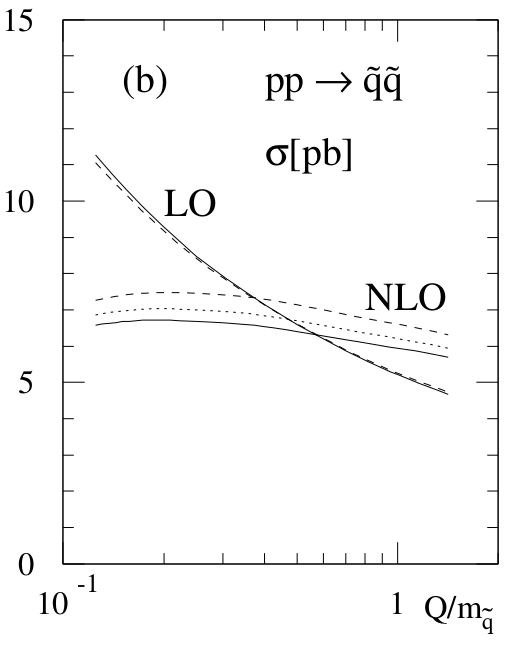
\includegraphics[scale=0.4]{figures_susy_at_hadron_colliders/squark_gluino_LO_NLO.png}
\caption[Renormalization scale dependence of LO and NLO cross sections]{The dependence on the renormalization scale $Q$ for the LO and NLO cross sections for squark-squark production at the LHC ($\sqrt{s}=14$ TeV). Parton densities are GRV94 (solid), CTEQ3 (dashed) and MRS(A') (dotted). Mass parameters are $m_{\widetilde{q}}=600$ GeV, $m_{\widetilde{g}}=500$ GeV and $m_t=175$ GeV. Figure from \cite{Beenakker:1996ch}.}
\label{Fig:: hadron susy : LO vs NLO beenakker}
\end{figure}

The NLO cross sections are calculated in \cite{Beenakker:1996ch}, assuming degenerate squark masses $m_{\widetilde{q}}$, with the five lightest quark masses set to zero, and the top quark mass to $m_t =175$ GeV. The two free parameters left in the cross sections are then $m_{\widetilde{g}}$ and $m_{\widetilde{q}}$, as seen in Eq.~(\ref{Eq:: susy hadron : Born term sigma}). The renormalization scheme used is the $\overline{MS}$ scheme. 



\subsubsection{Next-to-leading Order Partonic Cross-Section}

As discussed in Sec.~\ref{Sec:: susy hadron : Hadron Colliders}, cross sections for hadron colliders require first finding the partonic cross sections. In order to analyze these, scaling functions are introduced \cite{Beenakker:1996ch} giving the general LO+NLO result for all strong production processes as
\begin{align}\label{Eq:: susy hadron : Partonic cross section LO+NLO}
\hat{\sigma}_{ij} = \frac{\alpha_s^2(Q^2)}{m^2} \Big\{ &f^B_{ij}(\eta, r) + 4 \pi \alpha_s (Q^2) \Bigg[ f_{ij}^{V+S}(\eta, r, r_t) \nonumber \\ & + f_{ij}^H (\eta, r) + \bar{f}_{ij} (\eta, r) \log \Bigg( \frac{Q^2}{m^2}\Bigg) \Bigg] \Big\},
\end{align}
where $Q^2$ is the renormalization scale discussed previously, often set to $Q^2 = m^2$, where $m = (\sqrt{p_1^2}~+~\sqrt{p_2^2})/2$ is the average mass of the produced particles. The partonic cross section is written as a function of the parameters
\begin{align}
&\eta = \frac{s}{4m^2} -1, &r= \frac{m_{\widetilde{g}}^2}{m_{\widetilde{q}}^2}, &&r_t = \frac{m_t^2}{m^2}.
\end{align} 

The scaling functions $f$ are as follows: the Born term $f^B$ from Eq.~(\ref{Eq:: susy hadron : Born term sigma}), the hard gluon corrections $f^H$, the scale-dependent contributions $\bar{f}$ and the sum of virtual and soft-gluon corrections $f^{V+S}$. The gluon corrections come from adding a final state gluon to the partonic reaction
\begin{align}
q_i q_j \rightarrow \widetilde{q}_i  \widetilde{q}_j g.
\end{align}

The energy near the threshold is the base for an important part of the contributions to the total cross section \cite{Beenakker:1996ch}. In this region the scaling functions can be expanded in the low velocity of produced particles $\beta$, leading to the following expressions for squark pair production \cite{Beenakker:1996ch}
\begin{align}
&f_{qq}^B = \frac{8 \pi \beta m_{\widetilde{q}}^2 m_{\widetilde{g}}^2}{27(m_{\widetilde{q}}^2 + m_{\widetilde{g}}^2)^2}, &&f_{q'q}^B = \frac{8 \pi \beta m_{\widetilde{q}}^2 m_{\widetilde{g}}^2}{9(m_{\widetilde{q}}^2 + m_{\widetilde{g}}^2)^2} \nonumber \\
& f_{qq}^{V+S} = f_{qq}^B \frac{1}{24 \beta} && f_{q'q}^{V+S} = f_{q'q}^B \frac{1}{24 \beta} \nonumber \\
&f_{qq}^H = f_{qq}^B \Big[\frac{2}{3 \pi^2} \log^2(8 \beta^2) - \frac{7}{2 \pi^2} \log (8 \beta^2) \Big] &&f_{q'q}^H = f_{q'q}^B \Big[\frac{2}{3 \pi^2} \log^2(8 \beta^2) - \frac{19}{6 \pi^2} \log (8 \beta^2) \Big] \nonumber \\
& \bar{f}_{qq} = - f_{qq}^B \frac{2}{3 \pi^2} \log (8 \beta^2) &&\bar{f}_{q'q} = - f_{q'q}^B \frac{2}{3 \pi^2} \log (8 \beta^2).\label{Eq:: susy hadron : Scaling functions near threshold}
\end{align}

To find the total cross section, the partonic cross section is then integrated over, as discussed in Sec.~{\ref{Sec:: susy hadron : Parton Distribution Functions}. In \cite{Beenakker:1996ch} the integrals are calculated numerically using the VEGAS integration routine \cite{PETERLEPAGE1978192}.


\subsubsection{K-Factor}

To quantify the change in the cross section from adding NLO terms, the \textit{$K$-factor}\nomenclature[P]{$K$-factor}{Ratio between LO and NLO cross sections} is introduced. The $K$-factor is the ratio between the cross sections
\begin{align}
K = \sigma_{NLO}/\sigma_{LO}.
\end{align}
The $K$-factor for squark production for varying mass ratios $m_{\widetilde{q}}/m_{\widetilde{g}}=2.0$, $ 1.6$, $1.2$, $0.8$ at the LHC at $\sqrt{s}=14~\mathrm{TeV}$ is shown in Fig.~\ref{Fig:: susy hadron : K-factor LHC}. As seen from the figure, the $K$-factor is larger than one and quite stable as a function of the squark mass. 

\begin{figure}
\centering
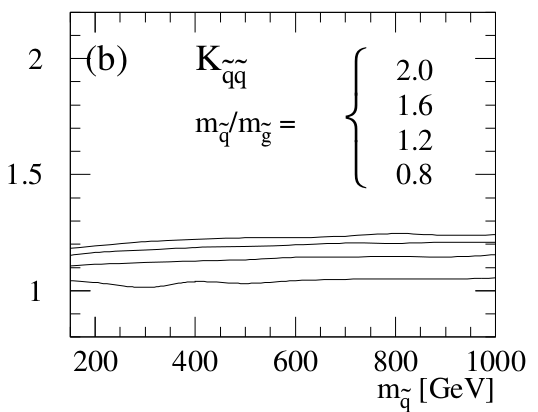
\includegraphics[scale=0.5]{figures_susy_at_hadron_colliders/squark_gluino_K_factor.png}
\caption[$K$-factors for the LHC]{$K$-factors for the LHC ($\sqrt{s}=14$ TeV). Parton densities are GRV94, with scale $Q=m$, and the top squark mass is $m_t=175$ GeV. Figure from \cite{Beenakker:1996ch}.}
\label{Fig:: susy hadron : K-factor LHC}
\end{figure}


\subsection{State-of-the-art Tools}

There are two current numerical tools for the calculation of NLO supersymmetric cross sections, namely \verb|Prospino 2.1| \cite{Beenakker:1996ed} and \verb|NLL-fast 2.1| \cite{Beenakker:2015rna}.

\subsubsection{Prospino}\label{Sec:: susy hadron : Prospino}
\verb|Prospino 2.1| \cite{Beenakker:1996ed} is a numerical tool that calculates supersymmetric cross sections to next-to-leading order for non-degenerate squark masses. First the LO cross sections are calculated for the five or four lightest squark flavours. The LO and NLO cross sections are then calculated for the mean value of the squark masses, and the corresponding $K$-factor is calculated. The LO cross sections for the individual squark processes are multiplied by the $K$-factor, giving an approximation to the NLO terms for non-degenerate masses. The calculation of NLO cross sections for squark production is outlined in the section above, and described in more detail in \cite{Beenakker:1996ed}. 

\verb|Prospino 2.1| assumes a particular renormalization scale to calculate cross sections. The uncertainty from the scale dependence is estimated in \verb|Prospino 2.1| by calculating cross sections for twice and half the chosen renormalization scale, and seeing how the cross sections change. As demonstrated in Fig.~\ref{Fig:: hadron susy : LO vs NLO beenakker}, the scale dependence of cross sections is reduced by adding higher order terms. As a consequence, the scale dependence is also a way of estimating the size of the contribution of higher order terms. 


As was discovered during the project, \verb|Prospino 2.1| has a technical weakness in the heavy squark mass space. \verb|Prospino 2.1| sets the NLO cross sections to zero when the mean squark mass is above threshold ($m^2 > s$). For individual masses \textit{below} the threshold, with nonzero leading order cross sections, this means inconsistently setting NLO cross sections to zero. This creates unphysical points --- or outliers --- in the dataset.

Evaluating cross sections with \verb|Prospino 2.1| is also highly time-consuming. Evaluating all the strong process cross sections for a single CMSSM benchmark point takes about 15 minutes of CPU time on a modern processor \cite{Balazs:2017moi}. 


\subsubsection{NLL-fast}

\verb|NLL-fast 2.1| \cite{Beenakker:1996ch, Kulesza:2008jb, Kulesza:2009kq, Beenakker:2009ha, Beenakker:2011fu} computes the hadronic cross sections of gluino and squark pair production including NLO QCD corrections, and the resummation of soft gluon emission at next-to-leading-logarithmic (NLL)\nomenclature[P]{NLL}{Next-to-leading-logarithmic order} accuracy. It also provides an error estimation, based on the errors from renormalization scale dependence and the parton distribution functions. The calculation is done by reading in tables of pre-calculated LO and NLO+NLL results, the scale uncertainty and the PDF and $\alpha_s$ error, and using fast grid interpolation to calculate cross sections for any squark and gluino mass in the range $[200, 2500]$ GeV for $\sqrt{s}=8~\mathrm{TeV}$. 

\verb|NLL-fast 2.1| is limited in that it only calculates cross sections for mass-degenerate squarks. Since the total cross section for squark pair production consists of 36 different cross sections for combinations of the four lightest quarks, the estimate from \verb|NLL-fast 2.1| is very simplified and unfit, \textit{e.g.} for the MSSM-24 as will be demonstrated in Sec.~\ref{Sec:: results : Cross Sections}.

\subsubsection{Accuracy}

Including the NLO+NLL partonic contributions has reduced the theoretical error to below $10 \%$ for a wide range of processes and masses, see the discussion in \cite{Balazs:2017moi}. There are other uncertainties, from the parton distribution functions (PDFs) and $\alpha_s$. These must also be included in the total error estimate. PDFs are based on experimental data, so the uncertainty increases with the sparticle masses because the PDFs are most poorly constrained at large scales $Q$ and at large parton $x$. However, with new data from the LHC errors from PDFs and $\alpha_s$ will be reduced over time.

On the basis of this, in order to keep the regression errors subdominant, the goal is that the relative regression errors obtained in this thesis should not exceed $10 \%$.







\chapter{Gaussian Processes}\label{Chapter:Gaussian Processes}

%\begin{chapquote}{Mark Twain}
%``Facts are stubborn things, but statistics are pliable."
%\end{chapquote}


In this chapter Gaussian process regression is introduced. First, some concepts and terminology in Bayesian statistics are reviewed. Then the concept of covariance, and how it can be determined by covariance functions is explored. Thereafter, the mathematical framework of Gaussian processes is introduced, and the Gaussian noise model is used as an example. Bayesian model selection and cross validation are introduced as tools to quantify and improve the quality of predictions.

\section{Introduction to Bayesian Statistics}

There are two general philosophies in statistics, namely \textit{Bayesian} and \textit{frequentist} statistics. Statisticians from both branches would probably consider the following statement to be true
\begin{quote}
\textit{Statisticians use probability to describe uncertainty.}
\end{quote}
The difference between Bayesian and frequentist statistics lies in the definition of the \textit{uncertain}. Since uncertainty is described by probability, the definition of probability must also differ. A distinction is made between \textit{objective} and \textit{subjective} probability. The former is used by frequentists, and Bayesians use a combination of the two. Consider an example in which a statistician throws a die. Before throwing, he is uncertain about the outcome of the toss. This uncertainty related to the outcome is \textit{objective}: no one can know if he will throw a 1 or a 4. On the other hand, he might also be uncertain about the underlying probability distribution of the toss. Is the die loaded? Is one of the edges sharper than the others? This uncertainty is \textit{subjective}, as it may vary depending on how much information is available about the system, and how that information is used. 

One of the main critisisms of subjective probability posed by frequentists is that the final probability depends on who you ask.

\subsection{Bayes' Theorem}

The difference between frequentist and Bayesian statistics also lies in the application of \textit{Bayes' theorem} \cite{mr1763essay}. Bayes' theorem can be derived from the familiar rules of probability for random variables $X$ and $Y$ given the information $I$,
\begin{align}\label{Eq:: gaussian process : Sum rule}
P(X | I) + P(\bar{X} | I) = 1,
\end{align}
\begin{align}
 \label{Eq:: gaussian process : Product rule}
P(X, Y | I) = P(X | Y, I)  P(Y | I),
\end{align} 
commonly known as the \textit{sum rule} and \textit{product rule}, respectively. The probability $P(X|I)$ is the probability of outcome $X$ given the information $I$, and $P(X|Y,I)$ is the probability of outcome $X$ given the information $I$ \textit{and} outcome $Y$. The bar over $\bar{X}$ means that the outcome $X$ does \textit{not} happen. The sum rule states that the total probability of the outcomes $X$ and $\bar{X}$ is equal to 1. This is rather intuitive, considering that an event either takes place or not. The product rule concerns the probability of both outcomes $X$ and $Y$. This is equal to the probability of $Y$ times the probability of $X$ given that $Y$ has already occurred. 

The product rule can be used to derive Bayes' theorem, first formulated by Thomas Bayes,
\begin{align}\label{Eq:: gaussian process : Bayes theorem}
P(Y | X, I) = \frac{P(X | Y, I)  P(Y | I)}{P(X | I)}.
\end{align}
Bayes' theorem states that the probability of $Y$ given $X$ is proportional to the probability of $X$ given $Y$, times the probability of $Y$. The proportionality factor is one over the probability of $X$. Surprisingly, there is nothing Bayesian --- in the modern statistical sense ---  about Bayes' theorem.  

In Bayesian statistics the theorem is used to perform inference about probability distributions. Probability distributions are functions that describe how the probability of a random variable $X$ is distributed, and are here denoted $P(X| \Theta, I)$. The \textit{parameters}, $\Theta$, of these functions determine the shape of the distribution, and are \textit{not} random variables. In physics, measurements are often used to find out more about the model. For example, data from the LHC is used to find the top mass $m_t$. The LHC data are then the variables $X$, and $m_t$ is the parameter $\Theta$. 

Bayes' theorem can be used to find the probability of the \textit{parameters} $\Theta$ given a set of random variables  $X$ drawn from the distribution. The resulting expression is the \textit{posterior probability distribution}\nomenclature[S]{$P(\Theta | X , I)$}{Posterior probability distribution}
\begin{align}\label{Eq:: gaussian process : Bayesian inference}
P(\Theta | X , I) = \frac{P(X|\Theta, I) P(\Theta| I)}{P(X | I)},
\end{align}
where $P(\Theta | I)$\nomenclature[S]{$P(\Theta | I)$}{Prior probability distribution}  and $P(X |\Theta, I)$\nomenclature[S]{$P(X |\Theta, I)$}{Likelihood function} are the \textit{prior} and \textit{likelihood}, respectively, and $P(X|I)$\nomenclature[S]{$P(X|I)$}{Marginal likelihood} is a normalization constant called the \textit{marginal likelihood}. 

The prior probability, $P(\Theta | I)$, represents the state of knowledge about the parameters given the background information $I$, before data has been analysed. In the example above, the prior would be the assumed top mass based on theoretical calculations in the SM. The prior is modified by the data through the likelihood, $P(X |\Theta, I)$, which is the probability of the data given the parameters.  The marginal likelihood is the probability of the data independently of the parameters, and can by Eq.~(\ref{Eq:: gaussian process : Product rule}) be written
\begin{align}
P(X|I) = \int P(X| \Theta, I) P(\Theta | I)~ \text{d} \Theta.
\end{align}
The marginal likelihood is revisited in Sec.~\ref{Sec:: gaussian process : Log Marginal Likelihood}.

In other words, Eq.~(\ref{Eq:: gaussian process : Bayesian inference}) states the probability of parameters $\Theta$ given the knowledge of outcomes $X$. The parameters $\Theta$ are sometimes called the \textit{hypothesis}, and the variables $X$ are called the \textit{evidence}. Bayes' theorem is then used to modify the hypothesis using the evidence. 



\subsection{Update of Belief}\label{Sec:: gaussian process : Priors and Likelihood}

The crucial parting of Bayesian statistics from frequentist statistics is the introduction of the \textit{prior}, and the possibility of updating the probability distribution using data. The prior expresses a \textit{prior} belief or assumption of the parameters given the background information, and has to be decided on beforehand. 

As mentioned previously, the measure $P(\Theta | X , I)$ from Eq.~(\ref{Eq:: gaussian process : Bayesian inference}) is called the posterior distribution. This can be thought of as the prior belief, modified by how well this belief fits the data, wich is decided by the likelihood,
\begin{align*}
\text{posterior} = \frac{\text{prior} \times \text{likelihood}}{\text{marginal likelihood}}.
\end{align*}

Consider an example. The statistician mentioned before now sets about tossing a coin. Before tossing he assumes the probability of heads as uniformly distributed, because is of the suspicious kind of statisticians. He therefore adopts a flat, or uniform, prior probability distribution. The uniform distribution is illustrated in the first panel in Fig.~\ref{Fig:: gaussian process : Dice throw }. After one toss he gets heads, and the posterior changes to a function with high probability for heads, and low for tails, illustrated in the second panel. After four tosses, of which two gave heads and two gave tails, the posterior in the third panel shows an equal probabilty for heads and tails, with a wide distribution centered at 0.5. After several tosses the distribution converges to a narrow peak around $0.25$, illustrated in the fourth panel. This indicates an unfair coin that is biased towards tails.

As seen from the example, Bayes' theorem can be used to iteratively update the posterior probability. After one coin toss, the distribution in the second panel of in Fig.~\ref{Fig:: gaussian process : Dice throw } can be thought of as the new prior, which is in turn modified by more tosses.

\begin{figure}
\includegraphics[scale=0.77]{figures_gaussian_processes/coin_toss_xd.pdf}
\caption[Priors and posteriors of a coin toss experiment]{The posterior probability distribution of the bias-weighting of a coin for the uniform prior, $P(H|I)$. The first panel from the left is before the coin is tossed, the second panel is after 1 toss, the third is after 4 tosses, and the fourth is after 1024 tosses. The posterior converges towards a narrow peak at $0.25$, so the coin is biased.}
\label{Fig:: gaussian process : Dice throw }
\end{figure}


\subsection{Best Estimate and Reliability}\label{Sec:: gaussian process : Best estimate}

The quantity of interest, such as the parameters of a distribution, will from now on be denoted $X$. Given a posterior distribution $P(X| \mathcal{D}, I)$ over $X$, where the prior given some information $I$ has been modified by some data $\mathcal{D}$, the posterior can be approximated by a Gaussian distribution with a \textit{mean} and \textit{variance}. 

The formal definition of the \textit{mean value} of $X$, denoted $m[X]$\nomenclature[S]{$m[X]$}{The mean value of the variable $X$}, is given by the \textit{expectation value} $\mathbb{E}[X]$\nomenclature[S]{$\mathbb{E}[X]$}{The expectation value of the variable $X$}. The mean value of a variable $X$ following a probability distribution $P(X |  I)$ is then defined as
\begin{align}\label{Eq:: gaussian process : Expectation value}
m[X] = \mathbb{E}[X] = \int X P(X | I) ~\text{d}X .
\end{align}

The variance $\mathbb{V} [X]$\nomenclature[S]{$\mathbb{V}[X]$}{The variance in the variable $X$} is defined as the expectation value of the square of deviations from the mean. If the mean value is $X_0$, the variance of $X$ following a probability distribution $P(X | I)$ is then given by 
\begin{align}\label{Eq:: gaussian process : variance X 1dim}
\mathbb{V}[X] = \mathbb{E} \big[ (X - X_0)^2 \big] = \int  (X - X_0)^2 P (X| I) ~\text{d}X.
\end{align}

The variance in $X$ is often denoted $\sigma_X^2 = \mathbb{V}[X]$, and its square root is the \textit{standard deviation} $\sqrt{\sigma^2_X} = \sigma_X$. The variance can be generalised to distributions over several variables. The variance of one quantity can then affect the variance of another. This correlation is called \textit{covariance}, and is discussed in Sec.~\ref{Sec:: gaussian process : Covariance}.

Returning to the posterior distribution $P(X | \mathcal{D}, I)$, the mean and variance of the approximated Gaussian distribution are given by the \textit{best estimate} and \textit{reliability}, respectively. The best estimate $X_0$  is the outcome with the highest probability. In other words, it maximises the posterior distribution
\begin{align}\label{Eq:: gaussian process : max of posterior}
&\frac{dP}{dX}\Big|_{X_0} = 0, &\frac{d^2P}{dX^2}\Big|_{X_0} < 0,
\end{align}
where $P$ is the posterior $P(X| \mathcal{D}, I)$. The second derivative must be negative to ensure that $X_0$ is, in fact, a maximum. 

Once a best estimate is found, it is important to know how reliable it is. Reliability, or uncertainty, is related to the width of the distribution. The width of the distribution indicates how much the posterior distribution is smeared out around the best estimate $X_0$. A narrow distribution has low uncertainty, while a wide distribution has large uncertainty. As an example, the third panel in Fig.~\ref{Fig:: gaussian process : Dice throw } shows a distribution with a mean value of $0.5$ with large uncertainty, while the fourth panel shows a distribution with mean $0.25$ with small uncertainty. 

The width is found by taking the logarithm\footnote{$L$ is a monotonic function of $P$, so the maximum of $L$ is at the maximum of $P$.} and Taylor expanding the posterior distribution $P(X| \mathcal{D}, I)$ around $X_0$. From Eq.~(\ref{Eq:: gaussian process : max of posterior}) the condition of the best estimate is that $dL/dX|_{X_0} =0$, so the expansion is given by
\begin{align}
&L = L(X_0) + \frac{1}{2} \frac{d^2L}{dX^2}\Big|_{X_0} (X-X_0)^2 +... ,&L = \log_e \Big[P(X | \mathcal{D}, I ) \Big]\label{Eq:: gaussian process : Taylor expansion L}
\end{align}
The first term, $L(X_0)$, is just a constant and can be absorbed in the normalisation. The dominant term in determining the width is therefore the quadratic term in Eq.~(\ref{Eq:: gaussian process : Taylor expansion L}).

Taking the exponential of Eq.~(\ref{Eq:: gaussian process : Taylor expansion L}) and ignoring higher order terms, the posterior can be approximated as
\begin{align}\label{Eq:: gaussian process : approximate Gaussian}
P(X | \mathcal{D}, I) \approx A \exp \Bigg[ \frac{1}{2} \frac{d^2L}{dX^2}\Big|_{X_0} (X-X_0)^2 \Bigg], 
\end{align} 
where $A = \exp \big[L(X_0) \big]$ is a constant. Equation~(\ref{Eq:: gaussian process : approximate Gaussian}) is now in the shape of a \textit{Gaussian distribution}.


\subsubsection{The Gaussian Distribution}\label{Sec:: gaussian process : The Gaussian Distribution}

\begin{figure}
\centering
\includegraphics[scale=1.0]{figures_gaussian_processes/gaussian_distribution_xd.pdf}
\caption[The general Gaussian distribution]{A Gaussian probability distribution. The maximum is at the mean value $\mu$, with a full width at half maximum (FWHM) at around $2.35 \sigma$. }
\label{Fig:: gaussian process : Gaussian distribution}
\end{figure}

The general \textit{Gaussian distribution} is given by
\begin{align}
P(X| \mu, \sigma^2) = \frac{1}{\sigma \sqrt{2 \pi}} \exp \Bigg[ - \frac{(X- \mu)^2}{2 \sigma^2} \Bigg],
\end{align}
where $\mu$ and $\sigma^2$ are the two parameters of the Gaussian distribution mentioned above. An example of a Gaussian distribution is shown in Fig.~\ref{Fig:: gaussian process : Gaussian distribution}. The parameter $\mu$ is the mean value of $X$ defined in Eq.~(\ref{Eq:: gaussian process : Expectation value}), $ m[X]$, and $\sigma^2$ is the variance of the distribution around the mean defined in Eq.~(\ref{Eq:: gaussian process : variance X 1dim}), $\mathbb{V}[X]$.  

The mean and variance for the approximated Gaussian distribution of the posterior $P(X|\mathcal{D}, I)$ are then given by
\begin{align}
m[X] = X_0\text{, }~ \mathbb{V}[X] = \Big( - \frac{d^2L}{dX^2} \Big)^{-1/2}.
\end{align}

The Gaussian distribution is also referred to as the \textit{normal distribution}, and a Gaussian distribution with mean $\mu$ and variance $\sigma^2$ is therefore denoted $\mathcal{N}(\mu, \sigma^2)$\nomenclature[S]{$\mathcal{N}(\mu, \sigma^2)$}{A Gaussian distribution with mean $\mu$ and variance $\sigma^2$}. The notation $Y \sim \mathcal{N}(\mu, \sigma^2)$\nomenclature[S]{$Y \sim \mathcal{N}$}{A variable $Y$ drawn from a Gaussian distribution} means a \textit{random variable $Y$ drawn from a Gaussian distribution with mean $\mu$ and variance $\sigma^2$}. The Gaussian distribution is symmetric with respect to the maximum at the mean $\mu$, and has a full width at half maximum (FWHM) at around $2.35 \sigma$, as seen in Fig.~\ref{Fig:: gaussian process : Gaussian distribution}.  



\subsubsection{Covariance}\label{Sec:: gaussian process : Covariance}




In distributions over several quantities of interest $X_i,~i=1,...,N$, called \textit{multivariate distributions} and denoted $P(X_i| \mathcal{D}, I)$, the \textit{covariance} denotes how much the variance of one quantity $X_p$ affects the variance of another quantity $X_q$. The covariance between $X_p$ and $X_q$ is denoted $\mathrm{cov}(X_p, X_q)$\nomenclature[S]{$\mathrm{cov}(X_p, X_q)$}{The covariance of $X_p$ and $X_q$}, and given by the expectation value of the product of deviations from the means for all quantities of interest $X_i$ 
\begin{align}\label{Eq:: gaussian process : Covariance definition}
\mathrm{cov}(X_p, X_q) &= \mathbb{E} \big[(X_p - {X_p}_0) (X_q - {X_q}_0) \big] \nonumber \\&=\int (X_p - {X_p}_0) (X_q - {X_q}_0) P (X_i | \mathcal{D}, I) ~\text{d}X_i.
\end{align}
Note that the covariance of $X_p$ with itself is the variance, $\mathrm{cov}(X_p, X_p) = \sigma_p^2$, so $\sigma_p^2$ is on the diagonal.

The covariance indicates how the variance of one quantity affects another quantity. If, for example, a high value for the variable $X_p$ leads to a high value of $X_q$, the covariance is positive. An example of positive covariance is shown in the third panel of Fig.~\ref{Fig:: gaussian process : Covariance illustrated}. The covariance is also positive if a low value for $X_q$ leads to a low value for $X_q$. If the value for $X_p$ has little or no effect on $X_q$, the covariance is negligible or zero $|\sigma_{X_pX_q}| \ll \sqrt{\sigma_{X_p}^2 \sigma_{X_q}^2}$, as seen in the first panel of Fig.~\ref{Fig:: gaussian process : Covariance illustrated}. The second panel shows negative covariance, where a high value for $X_p$ leads to a low value for $X_q$.


\begin{figure}
\centering
\includegraphics[scale=1.0]{figures_gaussian_processes/covariance_xd.pdf}
\caption[An illustration of covariance]{A schematic illustration of covariance and correlation. The contours of equiprobability of a posterior with zero covariance (left), where the inferred values of $X$ and $Y$ are uncorrelated. The corresponding plot when the covariance is large and negative (middle), and large and positive (right).}
\label{Fig:: gaussian process : Covariance illustrated}
\end{figure}

\subsubsection{Multivariate Best Estimate}

For multivariate distributions the best estimate is not as simple to solve for as in Eq.~(\ref{Eq:: gaussian process : Taylor expansion L}). A set of \textit{simultaneous equations} must be solved to get the best estimate
\begin{align}\label{Eq:: gaussian process : Best estimate X_i}
&\frac{dP}{dX_i} \Big|_{X_{j0}} =0, &&\frac{d^2P}{dX_i^2} \Big|_{X_{j0}} < 0,
\end{align}
for all $i=1,...,N$.

For simplicity the multivariate distribution is considered in two dimensions, where $\{ X_i \}=(X, Y)$. As in Eq.~(\ref{Eq:: gaussian process : Taylor expansion L}), the Taylor expansion of the logarithm of the posterior, $L = \log_e \Big[ P(X, Y |\mathcal{D}, I) \Big]$, is used to determine the reliabilities of the best estimates
\begin{align}\label{Eq:: gaussian process : Taylor expansion L_i}
L =& L(X_0, Y_0) + \frac{1}{2} \Big[ \frac{d^2L}{dX^2}  \Big|_{X_0, Y_0}(X-X_0)^2 \nonumber \\
& + \frac{d^2L}{dY^2}  \Big|_{X_0, Y_0}(Y-Y_0)^2 + 2 \frac{d^2L}{dXdY}  \Big|_{X_0, Y_0}(X-X_0)(Y-Y_0) \Big] +...
\end{align}
Again, the term $L(X_0, Y_0)$ is a constant, and the first derivatives are zero from the condition in Eq.~(\ref{Eq:: gaussian process : Best estimate X_i}), so the reliability is given by the second derivatives. There are four partial derivatives, reduced to three using the rules for mixed partial derivatives $\frac{\partial^2}{\partial X \partial Y} = \frac{\partial^2}{\partial Y \partial X}$. Writing the quadratic terms of Eq.~(\ref{Eq:: gaussian process : Taylor expansion L_i}) in matrix form gives
\begin{align}
Q = 
\begin{pmatrix}
X-X_0 & Y -Y_0
\end{pmatrix}
\begin{pmatrix}
A & C\\
C & B
\end{pmatrix}
\begin{pmatrix}
X -X_0\\
Y-Y_0
\end{pmatrix},
\end{align}
where the matrix elements are 
\begin{align}\label{Eq:: gaussian process : covariance matrix ABC}
&A = \frac{\partial^2 L}{\partial X^2} \Big|_{X_0, Y_0}, &B = \frac{\partial^2 L}{\partial Y^2} \Big|_{X_0, Y_0}, &&C = \frac{\partial^2 L}{\partial X \partial Y} \Big|_{X_0, Y_0}.
\end{align}
The widths, or reliabilities, can now be placed in the \textit{covariance matrix}.


\subsubsection{Covariance Matrix}

The variances and covariances are the elements of the \textit{covariance matrix}. For $N$ quantities of interest $X_1, ...,X_N$ the covariance matrix is an $N \times N$-matrix. The covariance matrix for $X$ and $Y$ is denoted $\text{cov}(X,Y)$, and it can easily be shown by exponentiation and comparison with the two-dimensional Gaussian that \cite{sivia2006data}
\begin{align}
\text{cov}(X,Y) = 
\begin{pmatrix}
\sigma_X^2 & \sigma_{XY}^2\\
\sigma_{XY}^2 & \sigma_Y^2
\end{pmatrix}
= - \begin{pmatrix}
A & C\\
C & B
\end{pmatrix}^{-1},
\end{align}
where $A$, $B$ and $C$ are the matrix elements of $Q$ defined in Eq.~(\ref{Eq:: gaussian process : covariance matrix ABC}),  $\sigma_X^2$ and $\sigma_Y^2$ are the variances of $X$ and $Y$, respectively, and $\sigma_{XY}^2$ is the covariance of $X$ and $Y$.

In short, the posterior probability distribution over $X$, $P(X | \mathcal{D}, I)$, can be approximated as a Gaussian distribution $\mathcal{N}(m[X], \mathbb{V}[X])$, where the mean is the best estimate and the variance is the associated reliability. The Gaussian distribution is defined by the mean value $m[X]$ and the variance $\mathbb{V}[X]$. For multivariate distributions, the covariance $\sigma_{X_i X_j}^2$ can also be calculated for the variables $X_i$, and all variances and covariances are contained in the covariance matrix $\text{cov}(X_i, X_j)$. When the exact form of the probability distribution is not known, the elements of a covariance matrix can also be calculated using assumed \textit{covariance functions} --- this lies at the heart of Gaussian processes.



\section{Covariance Functions}\label{Sec:: gaussian processes : Covariance functions}


The elements of a covariance matrix can be given by \textit{covariance functions}, or \textit{kernels}. In Gaussian processes these are used to calculate the covariance between function values, as will be shown in Eq.~(\ref{Eq:: gaussian process : cov(y) gaussian process}). Since functions can take vectors as arguments, $\textbf{x}$, the covariance functions are here also functions of input vectors $\textbf{x}$. A function that maps two arguments $\textbf{x},\textbf{x}' \in \mathcal{X}$ into $\mathbb{R}$, where $\mathcal{X}$ is the input space, is generally called a kernel $k$. Covariance functions are symmetric kernels, meaning that $k(\textbf{x}, \textbf{x}') = k(\textbf{x}', \textbf{x})$\nomenclature[S]{$k(\vec{x}, \vec{x}')$}{Kernel or covariance function}. In this thesis both terms, kernel and covariance function, refer to the covariance function. 


A kernel function that only depends on the difference between two points, $\textbf{x}-\textbf{x}'$, is called \textit{stationary}, \textit{i.e.} invariant to translations in input space. If, in addition, it only depends on the length $r=|\textbf{x}-\textbf{x}'|$, the function is \textit{isotropic}\footnote{Invariant to rigid rotations in input space.}.  

The covariance function can also depend on the dot product, $\textbf{x} \cdot \textbf{x}'$, and is then called a \textit{dot product} covariance function. The most important covariance functions for this thesis are the \textit{squared exponential covariance function} and the \textit{Mat\'{e}rn class of covariance functions}.




\subsection{The Squared Exponential Covariance Function}

The \textit{squared exponential covariance function} has the form 
\begin{align}\label{Eq:: gaussian process : Squared Exponential Kernel}
k_{\mathrm{SE}} (r) = \exp \Big( - \frac{r^2}{2 \ell^2} \Big),
\end{align} 
where $\ell$ is the \textit{characteristic length scale}. Equation~(\ref{Eq:: gaussian process : Squared Exponential Kernel}) is sometimes also called the \textit{radial basis function} (RBF)\nomenclature[S]{RBF}{The squared exponential kernel/the radial basis function}. The length scale, $\ell$\nomenclature[S]{$\ell$}{The characteristic length scale of a kernel}, determines the smoothness of the function. It can be loosely interpreted as how far you need to move (along a particular axis) in input space for the function values to become uncorrelated. For a large length scale one should expect a very slowly varying function, while a shorter length scale means a more rapidly varying function, see the illustration in Fig.~\ref{Fig:: gaussian process : ell variation example}. The RBF is infinitely differentiable and therefore very smooth. Stein \cite{stein2012interpolation} argues that such strong smoothness assumptions are unrealistic for most physical problems, and recommends another class of kernels, namely the \textit{Mat\'{e}rn class of covariance functions}.

\begin{figure}
\centering
\includegraphics[scale=1.5]{figures_gaussian_processes/length_scales_xd.pdf}
\caption[An illustration of length scales]{The effect of varying the length scale $\ell$. A long length scale (blue) gives a slowly varying function, while a short length scale (red) gives a more staccato, quickly varying function.}
\label{Fig:: gaussian process : ell variation example}
\end{figure}

%The SE is implemented in \verb|scikit-learn| under the name radial basis function (RBF), and may be called in the following way for length scale $10$, with bounds on the length scale $[0.01, 100]$
%\begin{lstlisting}
%from sklearn.gaussian_process.kernels import RBF
%rbf = RBF(length_scale=10, length_scale_bounds=(1e-2, 1e2))
%\end{lstlisting}

\subsection{The Mat\'{e}rn Class of Covariance Functions}\label{Sec:: gaussian process : Matern Class of Covariance Functions}

The \textit{Mat\'{e}rn class of covariance functions} is given by
\begin{align}\label{Eq:: gaussian process : Matern class of covariance functions}
k_{\mathrm{Mat\acute{e}rn}} (r) = \frac{2^{1- \nu}}{\Gamma (\nu)} \Big( \frac{\sqrt{2 \nu} r	}{\ell} \Big)^{\nu} K_{\nu} \Big( \frac{\sqrt{2 \nu}r}{\ell} \Big),
\end{align}
where $\nu, \ell > 0$, $K_{\nu}$ is a modified Bessel function \cite{abramowitz1964handbook}, and $\Gamma(\nu)$ is the gamma function. The hyperparameter $\nu$ controls the smoothness of the function. For $\nu \rightarrow \infty$ this becomes the RBF, and for $\nu = 1/2$ it becomes the very rough exponential kernel $k(r)= \exp (-r/\ell)$. In the case of half integer $\nu$, $\nu = p + \frac{1}{2}$ for $p \in \mathbb{N}$, the covariance function is simply the product of an exponential and a polynomial
\begin{align}
k_{\nu=p+\frac{1}{2}} = \exp \Big(- \frac{\sqrt{2 \nu} r	}{\ell} \Big) \frac{\Gamma(p+1)}{\Gamma(2p + 1)} \sum^p_{i=0} \frac{(p+i)!}{i!(p-i)!} \Big( \frac{\sqrt{8 \nu} r	}{\ell} \Big)^{p-i}.
\end{align}
In machine learning the two most commonly used cases are for $\nu = 3/2$ and $\nu = 5/2$
\begin{align}
k_{\nu = 3/2}(r) &=  \Big(1 + \frac{\sqrt{3}r}{\ell} \Big) \exp \Big( -\frac{\sqrt{3}r}{\ell} \Big),\\
k_{\nu = 5/2}(r) &=  \Big(1 + \frac{\sqrt{5}r}{\ell}  + \frac{5r^2}{3 \ell^2}\Big) \exp \Big( -\frac{\sqrt{5}r}{\ell} \Big).
\end{align}

%In \verb|scikit-learn| the hyperparameter $\nu$ is fixed, and so not optimized during training. The Mat\'{e}rn kernel is considered more appropriate for physical processes \cite{rasmussen2006gaussian}, and may be called in \verb|scikit-learn| in the following way for length scale 10, length scale bounds $[0.01, 100]$ and $\nu = 3/2$
%\begin{lstlisting}
%from sklearn.gaussian_process.kernels import Matern
%matern = Matern(length_scale=10, length_scale_bounds=(1e-2, 1e2), nu=1.5)
%\end{lstlisting}


\subsection{Noise}\label{Sec:: gaussian process : Noise Covariance Function}


The covariance function can also contain information about noise in the data. If the noise $\varepsilon$ follows a Gaussian distribution $\varepsilon \sim \mathcal{N}(0, \sigma_n^2)$, the noise can be represented by adding the variance, $\sigma_n^2$\nomenclature[S]{$\sigma_n^2$}{The variance of Gaussian distributed noise $\varepsilon$}, to the diagonal of the covariance matrix
\begin{align}
k(\textbf{x}_p, \textbf{x}_q)_{noise} = \sigma^2_n \delta_{pq},
\end{align}
where $\delta_{pq}$ is the Kronecker delta. The model where the noise is assumed to follow a Gaussian distribution is called the \textit{Gaussian noise model}, and is discussed further in Sec.~\ref{Sec: gaussian process : Gaussian Noise Model}. %In \verb|scikit-learn| this can be implemented either by giving a fixed noise level \verb|alpha| to the regressor function, or by using the \verb|WhiteKernel|, which estimates the noise level from the data. %This kernel is implemented in \verb|scikit-learn| in the following way for noise level $0.001$ with bounds $[10^{-10}, 1]$
%\begin{lstlisting}
%from sklearn.gaussian_processes.kernels import %WhiteKernel
%whitenoise = WhiteKernel(noise_level=0.001, noise_level_bounds=(1e-10,1))
%\end{lstlisting}

\subsection{Hyperparameters}\label{Sec:: gaussian process : Hyperparameters}

The RBF kernel in Eq.~(\ref{Eq:: gaussian process : Squared Exponential Kernel}) and the Mat\'{e}rn kernel in Eq.~(\ref{Eq:: gaussian process : Matern class of covariance functions}) are both isotropic, \textit{i.e.} they are functions only of the distance between input points, $r$. Isotropic kernels can, however, be generalised to an anisotropic form by setting
\begin{align}
r^2(\textbf{x}, \textbf{x}') = (\textbf{x} - \textbf{x}')^T M(\textbf{x} - \textbf{x}'),
\end{align}
where $M$ is a \textit{positive-definite} matrix. An $n \times n$ matrix is said to be positive-definite if the scalar $zMz^T$ is strictly positive for every non-zero column vector $z$ of $n$ real numbers. The matrix $M$ can take multiple forms, such as 
\begin{align}
M_1 = \ell^{-2} \mathbb{I} \quad \mathrm{or} \quad M_2 = \text{diag}(\vec{\ell})^{-2},
\end{align}
where $\ell^2$ is a scalar, and $\vec{\ell}$ is a vector of the same dimension as the input vector $\textbf{x}$. Choosing $\vec{\ell}$ to be a vector instead of a scalar is in many cases useful, especially if the input vector $\textbf{x}$ contains values of different scales.

The matrix $M$ is now part of the \textit{hyperparameters} of the kernel. Each kernel has a vector of hyperparameters, denoted $\vec{\theta}$\nomenclature[S]{$\vec{\theta}$}{The vector of hyperparameters for a kernel}. An example is the following generalisation of the RBF kernel, 
\begin{align}\label{Eq:: gaussian process : General RBF kernel}
k(\textbf{x}_p, \textbf{x}_q) = \sigma_f^2 \exp \big(- \frac{1}{2} (\textbf{x}_p - \textbf{x}_q)^T M (\textbf{x}_p - \textbf{x}_q) \big) + \sigma_n^2 \delta_{pq},
\end{align}
where $\sigma_f^2$ is a scaling factor and $\sigma_n^2$ is the Gaussian noise parameter, discussed in Sec.~\ref{Sec:: gaussian process : Noise Covariance Function}. The hyperparameters of this kernel are $\vec{\theta} = (\{M\}, \sigma^2_f, \sigma_n^2)^T$, where $\{M\}$ denotes the parameters in the symmetric matrix $M$. 
%The length scale can be set to a vector in \verb|scikit-learn| by giving the \verb|length_scale| parameter as a \verb|numpy| array of the same dimension as the input vector $\textbf{x}$.

\subsubsection{Other Covariance Functions}

There are several other types of covariance functions that are not discussed here. In addition, kernels can be multiplied and summed to form new kernels, making the space of possible kernels infinite. For further details see Chapter 4 in \cite{rasmussen2006gaussian}.




\section{Gaussian Process Regression}\label{Sec: gaussian process : Gaussian Process Regression}

Gaussian processes (GP) is a supervised machine learning method, designed to solve regression and probabilistic classification problems. Only regression is explored in this thesis. This section begins by introducing Gaussian processes and important notation. Then the prior and posterior distributions in Gaussian processes are considered, followed by a short discussion on how functions can be drawn from these distributions. Finally, a quick overview of the noise-free model and the Gaussian noise model are given.

\subsection{Basics and Notation}\label{Sec:: gaussian process : Basics and Notation}

%\subsubsection{Gaussian Processes}\label{Sec:: gaussian process : Gaussian Processes}

Consider a set of points $\mathcal{D} = \{\textbf{x}_i, y_i\}$\nomenclature[S]{$\mathcal{D} = \{\textbf{x}_i, y_i\}$}{Training dataset}, where $y$ is some (possibly noisy) function of $\textbf{x}$, $y(\textbf{x}) = f(\textbf{x}) + \varepsilon$. Here, $\varepsilon$ is the noise and $f(\textbf{x})$ is the true value of the function. These points are illustrated by the black dots in Fig.~\ref{Fig:: gaussian process : GP illustration}. In machine learning $\mathcal{D}$ is the \textit{training data}, as it is used to train the model. It consists of \textit{features}, which are the components of the input vectors $\textbf{x}_i$, and \textit{targets}, which are the function values $y_i$. The set of points is discrete, so there is some $\textbf{x}^*$\nomenclature[S]{$\textbf{x}^*$}{A test feature} for which the target $y^*$ is unknown. The test point $\textbf{x}^*$ is marked on the $x$-axis in Fig.~\ref{Fig:: gaussian process : GP illustration}.

Gaussian processes (GP) predict a Gaussian distribution \textit{over function values} at this point $\textbf{x}^*$. The distribution for a single test point $\textbf{x}^*$ has a corresponding mean $m(\textbf{x}^*)$ and variance $\mathbb{V}(\textbf{x}^*)$. Note that the mean $m(\textbf{x}^*)$ \textit{is not the mean of the input vector} $\textbf{x}^*$, but rather \textit{the mean of function values} $f(\textbf{x})$ \textit{evaluated at} $\textbf{x}^*$. 

The GP prediction for the target value $y^*=f(\textbf{x}^*)$ is the mean $m(\textbf{x}^*)$. Similarly, the variance, $\mathbb{V}(\textbf{x}^*)$, is in fact the variance in function values $f(\textbf{x}^*)$, or the width of the Gaussian distribution (red line) in the $y$-direction in Fig.~\ref{Fig:: gaussian process : GP illustration}. The mean value $y^*$ is drawn as a blue cross in Fig.~\ref{Fig:: gaussian process : GP illustration}. As will be shown, the predicted target $y^*$ is a linear combination of the known targets $y_i$, where the weights are controlled by the covariances between training points $\textbf{x}_i$ and the test point $\textbf{x}^*$.  


\begin{figure}
\centering
\includegraphics[scale=1.5]{figures_gaussian_processes/gp_illustration_xd.pdf}
\caption[An illustration of Gaussian process regression]{An illustration of a GP prediction of the target value $y^*$ (blue cross), given the known set of points $\{x_i, y_i\}$ (black dots). The prediction is a Gaussian distribution in $y$ with mean $y^*$ and variance $\sigma^2$. The Gaussian distribution is drawn in red with $y$ on the vertical axis, with uncertainty in the $y$-direction.}
\label{Fig:: gaussian process : GP illustration}
\end{figure}

\subsubsection{Some Notation}

As Gaussian process regression is notoriously confusing, it is helpful to begin with some notation. 

As introduced in Sec.~\ref{Sec: gaussian process : Gaussian Process Regression}, the Gaussian distribution with a mean $\mu$ and variance $\sigma^2$ is denoted $\mathcal{N}(\mu, \sigma^2)$. The distribution can be over a single random variable, $f$, or a finite set of random variables, $f_i$. A Gaussian distribution over several random variables is called a \textit{multivariate Gaussian distribution}. The $n$ random variables $f_i, ~i=1,...,n$, drawn from a multivariate Gaussian distribution make up the $n$-dimensional vector $\textbf{f}$\nomenclature[S]{$\vec{f}$}{Vector of latent function values for training data}. The mean values, $\mu_i$, are then contained in the $n$-dimensional \textit{mean vector} $m[\textbf{f}]$\nomenclature[S]{$m[\vec{f}]$}{The vector containing the mean values of $\vec{f}$}. The variance, $\sigma^2$, is replaced by an $n \times n$-dimensional covariance matrix, $\text{cov}(\textbf{f})$. The multivariate Gaussian distribution over $\textbf{f}$ is written as
\begin{align}
\textbf{f} \sim \mathcal{N} \big(m[\textbf{f}], ~\text{cov}(\textbf{f})  \big).
\end{align}  

For $n$ points $\{\textbf{x}_i , y_i\}$, where $\textbf{x}_i$ is an $m$-dimensional feature vector and $y_i$ is the target, the features comprise the $n \times m$-matrix $X$\nomenclature[S]{$X$}{Matrix containing training features}. The targets make up the corresponding $n$-dimensional vector $\textbf{y}$. The vector containing the latent function values, \textit{i.e.} $f_i = f(\textbf{x}_i)$, is denoted $\textbf{f}$. A central assumption in Gaussian process regression is that the covariance between targets $y_i$, $y_j$ is given by the kernel of their features $\textbf{x}_i$, $\textbf{x}_j$
\begin{align}\label{Eq:: gaussian process : cov(y) gaussian process}
\text{cov}(y_i, y_j) = k(\textbf{x}_i, \textbf{x}_j),
\end{align}
where $k(\textbf{x}_i, \textbf{x}_j)$ is a covariance function, as described in Sec.~\ref{Sec:: gaussian processes : Covariance functions}. In Gaussian processes the distribution over target values $\textbf{y}$\nomenclature[S]{$\vec{y}$}{Vector of noisy training target values} with feature matrix $X$ will therefore be written
\begin{align}\label{Eq:: gaussian process : Normal distribution GP}
\textbf{y} \sim \mathcal{N} \big(~m[ \textbf{y} ], K(X, X) ~\big),
\end{align}
where $K(X,X)$ is the covariance matrix containing the covariances of the features in $X$, calculated using the covariance function $k(\textbf{x}_i, \textbf{x}_j)$.

Finally, a Gaussian process will be denoted $\mathcal{GP}$. It may be difficult to distinguish between a Gaussian \textit{distribution}, $\mathcal{N}$, and a Gaussian \textit{process}, $\mathcal{GP}$. The difference can be thought of as the difference between a finite collection of function values $f_i = f(\textbf{x}_i)$, and the continuous function, $f(\textbf{x})$. The former can be viewed as a vector $\textbf{f}$, and can be drawn from a distribution such as the one in Eq.~(\ref{Eq:: gaussian process : Normal distribution GP}), $\textbf{f} \sim \mathcal{N}(~m[\textbf{f} ], K(X, X)~)$. The latter is a \textit{function}, drawn from a distribution \textit{over functions}, where the mean $m(\textbf{x})$\nomenclature[S]{$m(\textbf{x})$}{Mean function for Gaussian processes}\footnote{Note that the mean \textit{function} of $\textbf{x}$ uses round brackets, $m(\textbf{x})$, while the mean \textit{value} of $\textbf{x}$ uses square brackets $m[\textbf{x}]$.} and covariances $k(\textbf{x}, \textbf{x}')$ are functions as well. A function $f(\textbf{x})$ drawn from a Gaussian process is written as\nomenclature[S]{$\mathcal{GP}$}{Gaussian processes} 
\begin{align}\label{Eq:: gaussian process : draw function from GP}
f(\textbf{x}) \sim \mathcal{GP} (m(\textbf{x}), k(\textbf{x}, \textbf{x}')).
\end{align}

\subsubsection{Function Space View}

Gaussian processes are distributions over functions. It is therefore useful to consider the problem in the function space view introduced in \cite{rasmussen2006gaussian}. For a function $f(\textbf{x})$ the Gaussian process \textit{mean function}, $m(\textbf{x})$, and \textit{covariance function}, $k(\textbf{x}, \textbf{x}')$, are defined as
\begin{align}
m(\textbf{x}) &= \mathbb{E}[f(\textbf{x})],\\
k(\textbf{x}, \textbf{x}') &= \mathbb{E} [(f(\textbf{x}) - m(\textbf{x}))(f(\textbf{x}') - m(\textbf{x}'))].
\end{align}

In other words, the mean $m(\textbf{x})$ is the expected value of the function $f(\textbf{x})$ at $\textbf{x}$, and the covariance function is the expected value of the simultaneous deviations of $f(\textbf{x})$ from the mean $m(\textbf{x})$ at $\textbf{x}$, and $f(\textbf{x}')$ from the mean $m(\textbf{x}')$ at $\textbf{x}'$. As mentioned, the mean and covariance are now \textit{functions} of the input vector $\textbf{x}$. This means that for every input vector $\textbf{x}$, there is a Gaussian distribution over function values with a mean $m(\textbf{x})$ and covariance with the function value at $\textbf{x}'$ given by $k(\textbf{x}, \textbf{x}')$. This is a generalization of the single test point in Fig.~\ref{Fig:: gaussian process : GP illustration}, where every point $\textbf{x}^*$ gets a similar distribution.

The collection of Gaussian distributions over functions that are now a function of the input vector $\textbf{x}$ are the Gaussian processes, $\mathcal{GP}$. In the same way that a random variable is drawn from a distribution, random functions can be drawn from the $\mathcal{GP}$, as shown in Eq.~(\ref{Eq:: gaussian process : draw function from GP}). How functions are drawn from the $\mathcal{GP}$ is discussed in more detail in Sec.~\ref{Sec:: gaussian process : the prior and posterior distribution}.

The covariance between $f(\textbf{x})$ and $f(\textbf{x}')$ is determined by a covariance function $k(\textbf{x}, \textbf{x}')$. As mentioned, the covariance function calculates the covariance between the \textit{function values}, $f(\textbf{x})$ and $f(\textbf{x}')$, and \textit{not} the input vectors, $\textbf{x}$ and $\textbf{x}$. Rather, the covariance between two function values is a function of the input vectors. Consider again the illustration in Fig.~\ref{Fig:: gaussian process : ell variation example}. The variation in function values $f(\textbf{x})$ and $f(\textbf{x}')$ depends on the distance between the points $\textbf{x}$ and $\textbf{x}'$, and the characteristic length scale of the process. If the length scale is large, the two input vectors $\textbf{x}$ and $\textbf{x}'$ can be far away, and still have similar function values $f(\textbf{x})$ and $f(\textbf{x}')$. For short length scales, however, nearby points can have very different function values, because the function varies rapidly.

\subsection{The Prior and Posterior Distribution}\label{Sec:: gaussian process : the prior and posterior distribution}



Gaussian processes are Bayesian in that there is a prior and a posterior distribution over functions, where the posterior is obtained by conditioning the prior on the training data. Consider the $n^* \times m$-matrix of test points $X^*$, containing $n^*$ test points $\textbf{x}_i^*$, with unknown function values $f(\textbf{x}^*)$. Using the kernel function, $k(\textbf{x}_i^*, \textbf{x}_j^*)$, on the matrix $X^*$\nomenclature[S]{$X^*$}{Matrix containing test features} gives the covariance matrix, $K(X^*, X^*)$, as discussed in Sec.~\ref{Sec:: gaussian processes : Covariance functions}. The covariance matrix  now contains the covariance of all test points $\textbf{x}^*_i$. Combined with an initial mean of zero\footnote{The mean does not have to be zero, it could for example be the mean of the training data.} one obtains the \textit{prior} distribution of predicted target values $\textbf{f}^*$
\begin{align}
\textbf{f}^* \sim \mathcal{N} (\vec{0}, K(X^*, X^*)).\label{Eq:: gaussian process : Prior GP}
\end{align} 
This distribution contains the prior assumptions about the function values $f(\textbf{x})$, in that the smoothness of the function and the correlation between function values are encoded in the covariance matrix. This is the prior probability distribution discussed in Sec.~\ref{Sec:: gaussian process : Priors and Likelihood}, that will be modified by the data to provide the posterior probability distribution. The choice of kernel is therefore one of the most important steps in learning with GPs. 

\subsubsection{Noise-Free Model}

Now consider the addition of training data to the prior distribution in Eq.~(\ref{Eq:: gaussian process : Prior GP}), in the form of a noise-free set of $n$ training points $\{\textbf{x}_i, y_i\}$, so that $y = f(\textbf{x})$. The input vectors $\textbf{x}_i$ form the $n \times m$-matrix $X$, where the rows are the input vectors. The training targets $y_i$ form a corresponding $n$-dimensional vector $\vec{y}$, which in the noise free case is equal to the latent function value vector $\textbf{f}$. The test points are still contained in the $n^* \times m$ matrix $X^*$. The goal is to predict an $n^*$-dimensional vector $\textbf{f}^*$ containing the predictions of the function values at the points $\textbf{x}^*_i$, which is conditioned on the known function values $\textbf{f}$. 

The joint distribution of training outputs, $\textbf{f}$, and test outputs, $\textbf{f}^*$, according to the prior in Eq.~(\ref{Eq:: gaussian process : Prior GP}) is
\begin{align}
\begin{bmatrix}
\textbf{f}\\
\textbf{f}^*
\end{bmatrix}
\sim 
\mathcal{N} \Bigg(
\boldsymbol{0},
\begin{bmatrix}
K(X, X) & K(X, X^*)\\
K(X, X^*) & K(X^*, X^*)
\end{bmatrix}
 \Bigg),
\end{align}
where, as before, $K(X_i, X'_j)$ is the covariance matrix between the sets of points $\{ \textbf{x}_i \}$ and $\{\textbf{x}'_j \}$ calculated using the covariance function $k(\textbf{x}_i, \textbf{x}'_j)$. By conditioning the distribution of $\textbf{f}^*$ on the observations $\textbf{f}$,  the posterior distribution over $\textbf{f}^*$ is obtained\footnote{For more details, see Appendix A.2 in \cite{rasmussen2006gaussian}.}  \cite{rasmussen2006gaussian} 
\begin{align}\label{Eq:: gaussian process : Posterior GP noise-free}
\textbf{f}^* \big| X^*, X, \textbf{f} \sim \mathcal{N}&(K(X^*, X)K(X, X)^{-1} \textbf{f}, \nonumber \\ &K(X^*, X^*) - K(X^*, X)K(X, X)^{-1}K(X, X^*)),
\end{align}
where $\textbf{f}^* | X^*, X, \textbf{f}$ means the target values $\textbf{f}^*$ for the features $X^*$, given the known features $X$ and targets $\textbf{f}$. The prior in Eq.~(\ref{Eq:: gaussian process : Prior GP}) has been modified by the data, $X$ and $\textbf{f}$, to give the posterior in Eq.~(\ref{Eq:: gaussian process : Posterior GP noise-free}), leaving two different distributions from which function values can be drawn before and after the data.


\subsubsection{Drawing Samples}

All functions $f(\textbf{x})$ that are drawn from the Gaussian process $\mathcal{GP}$ must have a covariance between function values $f(\textbf{x})$ and $f(\textbf{x}')$ determined by the covariance function $k(\textbf{x}, \textbf{x}')$.  The mean of the distribution, $m(\textbf{x})$, is \textit{not} the mean value of each function $f(\textbf{x})$ drawn from $\mathcal{GP}$, but rather the mean function value you would get at $\textbf{x}$ if you drew enough functions from the $\mathcal{GP}$. Drawing functions from a distribution in this way will be referred to as \textit{drawing samples}. The samples drawn here will in fact be function vectors $\vec{f}$ drawn from the normal distributions in Eq.~(\ref{Eq:: gaussian process : Prior GP}) and Eq.~(\ref{Eq:: gaussian process : Posterior GP noise-free}), and not functions $f(\textbf{x})$ from a Gaussian process $\mathcal{GP}(m(\textbf{x}), k(\textbf{x}, \textbf{x}'))$.

To generate samples $\textbf{f} \sim \mathcal{N}(\textbf{m}, K)$ with a mean vector $\textbf{m}$ and covariance matrix $K$ using a scalar Gaussian generator\footnote{A scalar Gaussian generator generates random numbers from a Gaussian distributions, and can be found in most programming enviroments, such as the \verb|random| environment in \verb|Python|.}, one proceeds as follows \cite{rasmussen2006gaussian}: first the Cholesky decomposition $L$ --- also known as the matrix square root ---  of the covariance matrix is found using $K = LL^T$, where $L$ is a lower triangular matrix. The Cholesky decomposition requires that the matrix $K$ be Hermitian and positive-definite.  A vector $\textbf{u}$ is then generated by multiple calls to the scalar Gaussian generator $\textbf{u} \sim \mathcal{N}(0, \mathbb{I})$. Then $\textbf{f} = \textbf{m} + L \textbf{u}$ has the desired distribution with mean $\textbf{m}$ and covariance
\begin{align}
\mathrm{cov}(\textbf{f}) = \mathbb{E}[(\textbf{f} - \textbf{m})(\textbf{f} - \textbf{m})^T] = \mathbb{E}[(L \vec{u})(L \vec{u})^T] = L \mathbb{E} [\textbf{u} \textbf{u}^T]L^T = LL^T = K
\end{align}
by the independence of the elements of $\vec{u}$.

Using the method described above, random function vectors have been drawn from the prior and posterior in Eq.~(\ref{Eq:: gaussian process : Prior GP}) and Eq.~(\ref{Eq:: gaussian process : Posterior GP noise-free}), respectively, and shown in Fig.~\ref{Fig:: gaussian process : prior posterior drawn samples}. As discussed, the samples drawn from the prior have mean equal to zero $m(\textbf{x})=\vec{0}$, and constant covariance, $K(X^*, X^*)$, meaning that if you drew enough function vectors the mean of all function values at every $\textbf{x}$ would be zero. The prior is shown in the upper panel of Fig.~\ref{Fig:: gaussian process : prior posterior drawn samples}, where the mean of the distribution is represented by the thick, black line, and the covariance is the light blue band around the mean. In the posterior distribution the mean values and covariances have been modified by the training data, represented by red dots in the lower panel of Fig.~\ref{Fig:: gaussian process : prior posterior drawn samples}. In a point where there is training data the uncertainty is zero\footnote{Assuming there is no noise in the data.}, and so all samples drawn from the posterior distribution must pass through this point. Far away from training points the covariance is large. The mean has also been modified to pass through the training points, as seen by the thick black line in the lower panel.

\begin{figure}
\centering
\includegraphics[scale=0.7]{figures_gaussian_processes/draw_samples_benchmark_ingrid.pdf}
\caption[Drawing samples from the Gaussian processes]{Drawing functions from the prior (top) and posterior (bottom) distributions as per the method described in Sec.~\ref{Sec:: gaussian process : the prior and posterior distribution}. The thick, black line represents the mean $m[\textbf{f}^*]$, while the shaded, blue area is the variance $K(X^*, X^*)$. The multiple coloured lines are functions drawn randomly from the prior and posterior distributions, whose correlation are dictated by the covariance function. Covariances are given by the RBF kernel $k(r) = \sigma_f^2 \exp(-r^2/\ell^2)$, and the prior has mean $\vec{0}$. The posterior (bottom panel) has been modified by training points (red dots), giving rise to zero uncertainty at the points where training data exists, and an altered mean value for the distribution. The kernel has hyperparameters $\sigma_f = 1$ and $\ell = 1$ for the prior, and $\sigma_f = 0.594$ and $\ell = 0.279$ for the posterior. Figure generated using {\tt scikit-learn 0.19.0}.}
\label{Fig:: gaussian process : prior posterior drawn samples}
\end{figure}

\subsubsection{Gaussian Noise Model}\label{Sec: gaussian process : Gaussian Noise Model}

Noise-free observations are rare. In most cases targets will contain some noise $y = f(\textbf{x}) + \varepsilon$, where the noise $\varepsilon$ is here assumed to follow a Gaussian distribution $\varepsilon \sim \mathcal{N}(0, \sigma_n^2)$. This is the \textit{Gaussian noise model}. As discussed in Sec.~\ref{Sec:: gaussian processes : Covariance functions} the covariance of a function with Gaussian noise can be expressed as
\begin{align}
&\text{cov}(y_i, y_j) = k(\textbf{x}_i, \textbf{x}_j) + \sigma_n^2 \delta_{ij}.
\end{align}
Training targets are contained in the $n$-dimensional vector $\textbf{y}$ --- which is now different from the latent function vector $\vec{f}$ --- while training features are contained in the $n \times m$-matrix $X$, test features in the $n^* \times m$-matrix $X^*$ and predicted targets in the $n^*$-dimensional vector $\textbf{f}^*$, as before. Note that the goal is to predict the function values $\vec{f}^*$, and \textit{not} the noisy values $\vec{y}^*$. 

With the addition of noise the prior distribution becomes
\begin{align}
\begin{bmatrix}
\textbf{y}\\
\textbf{f}^*
\end{bmatrix}
\sim 
\mathcal{N} \Bigg(
\boldsymbol{0},
\begin{bmatrix}
K(X, X) + \sigma_n^2 \mathbb{I} & K(X, X^*)\\
K(X, X^*) & K(X^*, X^*)
\end{bmatrix}
 \Bigg).
\end{align}
The conditioned distribution is then 
\begin{align}
\textbf{f}^* \big| X^*, X, \textbf{y} & \sim \mathcal{N}(m[\textbf{f}^*], \text{cov}(\textbf{f}^*))
\end{align}
where
\begin{align}
m[\textbf{f}^*] &= K(X^*, X) [K(X, X) + \sigma_n^2 \mathbb{I}]^{-1} \textbf{y},\label{Eq:: gaussian process : predicted mean}\\ 
\text{cov} (\textbf{f}^*) &= K(X^*, X^*) - K(X^*, X)[K(X, X) + \sigma_n^2 \mathbb{I}]^{-1} K(X, X^*), \label{Eq:: gaussian process : predicted variance}
\end{align}
which are similar to the mean and covariance in Eq.~(\ref{Eq:: gaussian process : Posterior GP noise-free}), but include noise in the covariance matrix. 

Equations~(\ref{Eq:: gaussian process : predicted mean}) and (\ref{Eq:: gaussian process : predicted variance}) are the key predictive equations for Gaussian process regression. The calculation requires inverting the $n \times n$-matrix containing the covariance $[K(X,X)~+~\sigma_n^2 \mathbb{I}]$, which for large $n$ becomes computationally unviable. This is discussed further in Sec.~\ref{Sec:: gaussian process : Distributed Gaussian Processes}, where distributed Gaussian processes are proposed as a way of scaling Gaussian processes to larger training sets.

To tidy up the expressions in Eqs.~(\ref{Eq:: gaussian process : predicted mean}) and (\ref{Eq:: gaussian process : predicted variance}) the covariance matrices $K\equiv K(X, X)$ and $K^* \equiv K(X, X^*)$ are defined. For a single test point $\textbf{x}^*$ the covariance matrix $K^*$ is written as a vector $\textbf{k}^* \equiv \textbf{k}(X, \textbf{x}^*) $ to denote the covariances between the $n$ training points and the test point $\textbf{x}^*$. Using this compact notation the GP prediction of $f^*=f(\textbf{x}^*)$ for a single test point $\textbf{x}^*$ is
\begin{align}
m[f^*] &= \textbf{k}^{*T}(K + \sigma_n^2\mathbb{I})^{-1} \textbf{y},\label{Eq:: gaussian process : GP prediction mean}\\
\mathbb{V}[f^*] &= k(\textbf{x}^*, \textbf{x}^*) - \textbf{k}^{*T}(K + \sigma_n^2 \mathbb{I})^{-1} \textbf{k}^*\label{Eq:: gaussian process : GP prediction variance}.
\end{align}
Note that, as intimated in Sec.~\ref{Sec:: gaussian process : Basics and Notation}, the predicted mean value $m[f^*]$ can be viewed as a linear combination of $y_i$ of the form $\alpha \textbf{y}$, where $\alpha = \textbf{k}^{*T}(K + \sigma_n^2\mathbb{I})^{-1}$. The vector $\alpha$ then only contains the covariance between features.

Equations (\ref{Eq:: gaussian process : GP prediction mean}) and (\ref{Eq:: gaussian process : GP prediction variance}) form the basis for GP prediction in the \verb|Python| library \verb|scikit-learn 0.19.0|  \cite{scikit-learn}. The algorithm for Gaussian process regression on a single test point $\textbf{x}^*$, with training data $X$, $\textbf{y}$ is outlined in Algorithm \ref{Alg:: gaussian process : GP}. The algorithm uses the Cholesky decomposition, $L$, of the covariance matrix to find the weights $\vec{\alpha}$ used to calculate the predictive mean $f^*$. The variance $\mathbb{V}[\textbf{x}^*]$ is calculated using $L$ and the covariance of the test point with the training points, $\textbf{k}^* = k(X, \textbf{x}^*)$.

\begin{algorithm}
\KwData{$X$ (training features), \textbf{y} (targets), $k$ (covariance function/kernel), $\sigma_n^2$ (noise level), $\textbf{x}_*$ (test feature).}
L = Cholesky decomposition ($K + \sigma_n^2 I$) \;
$\boldsymbol{\alpha} = (L^T)^{-1}(L^{-1} \textbf{y})$ \;
$f_* = \textbf{k}_*^T \boldsymbol{\alpha}$ \;
$\textbf{v} = L^{-1} \textbf{k}_*$ \;
$\mathbb{V}[f_*] = k(\textbf{x}_*, \textbf{x}_*) - \textbf{v}^T \textbf{v}$ \;
$\log p(\textbf{y}|X) = - \frac{1}{2} \textbf{y}^T \boldsymbol{\alpha} - \sum_i \log L_{ii} - \frac{n}{2} \log 2 \pi$ \;
\KwResult{$f_*$ (mean), $\mathbb{V}[f_*]$ (variance), $\log p(\textbf{y}|X)$ (log marginal likelihood).}
\caption{Algorithm 2.1 from \cite{rasmussen2006gaussian}.}
\label{Alg:: gaussian process : GP}
\end{algorithm}




\section{Model Selection}

Choosing the right kernel and hyperparameters is an important part of Gaussian process regression. Finding the  kernel and corresponding hyperparameters that best fit the data is often called \textit{model selection}. Model selection is also referred to as \textit{training} in machine learning. In this section Bayesian model selection for the marginal likelihood is quickly overviewed, and the log marginal likelihood and cross validation are introduced as tools to optimise Gaussian process estimators.



The \textit{marginal likelihood} can be used to find the optimal hyperparameters of covariance functions. Gaussian process regression with the Gaussian noise model described in Sec.~\ref{Sec: gaussian process : Gaussian Noise Model} has the wonderful trait of analytically tractable integrals for the marginal likelihood, $P(\textbf{y}|X, \boldsymbol{\theta})$. Note that the marginal likelihood defined here looks different than in Eq.~(\ref{Eq:: gaussian process : Bayesian inference}) --- $\boldsymbol{\theta}$ are the hyperparameters of the covariance functions introduced in Sec.~\ref{Sec:: gaussian process : Hyperparameters}, $\textbf{y}$ are the training outputs and $X$ are the training inputs. The parameters in Eq.~(\ref{Eq:: gaussian process : Bayesian inference}), there denoted $\Theta$, are now the true --- or \textit{latent} --- function values, $\textbf{f}$, where $\textbf{y} = \textbf{f} + \varepsilon$. 

The marginal likelihood is the integral of the likelihood times the prior over the latent function values $\textbf{f}$, given by
\begin{align}\label{Eq:: gaussian process : Marginal likelihood}
P(\textbf{y} | X, \boldsymbol{\theta}) = \int P(\textbf{y}| \textbf{f}, X, \boldsymbol{\theta}) P (\textbf{f}|X, \boldsymbol{\theta})d \textbf{f},
\end{align}
where $P(\textbf{f}|X, \boldsymbol{\theta})$ is the prior and $P(\textbf{y}|\textbf{f},X, \boldsymbol{\theta})$ is the likelihood. 

Under the Gaussian process model the prior is a Gaussian distribution $\textbf{f}| X, \vec{\theta} \sim \mathcal{N}(\textbf{0}, K + \sigma^2_n \mathbb{I})$, and the likelihood is $\vec{y} | \vec{f}, X, \vec{\theta} \sim \mathcal{N}(\vec{f}, \sigma_n^2 \mathbb{I})$. The logarithm of Eq.~(\ref{Eq:: gaussian process : Marginal likelihood}) then gives the \textit{log marginal likelihood} (LML)\nomenclature[S]{LML}{Log marginal likelihood} \cite{rasmussen2006gaussian} 
\begin{align}\label{Eq:: gaussian process : LML gaussian process}
\log P(\textbf{y}|X, \boldsymbol{\theta}) = - \frac{1}{2} \textbf{y}^T K_y^{-1} \textbf{y} - \frac{1}{2} \log \big|K_y| - \frac{n}{2} \log 2 \pi,
\end{align}
where $n$ is the number of training points, $K_y = K_f + \sigma_n^2 \mathbb{I}$ is the covariance matrix for the noisy targets $\vec{y}$, and $K_f$ is the covariance matrix for the latent function values $\vec{f}$. Each term in Eq.~(\ref{Eq:: gaussian process : LML gaussian process}) has an interpretation: $- \frac{1}{2} \textbf{y}^T K_y^{-1} \textbf{y}$ is the only term involving the data, and is therefore the data-fit; $-\frac{1}{2} \log \big| K_y \big|$ is the complexity penalty depending only on the covariance function and the inputs; and $- \frac{n}{2} \log 2 \pi$ is a normalization term. 



\begin{figure}[H]
\centering
\includegraphics[scale=0.5]{figures_gaussian_processes/LML_two_local_maxima_ingrid.pdf}
\caption[A contour plot of the LML]{A contour plot of the log marginal likelihood with two local optima for a Gaussian process with the kernel in Eq.~(\ref{Eq:: gaussian process : General RBF kernel}) for sample data. The rightmost optima favours a short length scale and low noise, with $\sigma_f~=~0.64$, $\ell = 0.365$ and $\sigma^2_n = 0.29$, while the leftmost favors a high noise level and therefore several large length scales, with $\sigma_f = 0.00316$, $\ell = 109$ and $\sigma^2_n = 0.6$. The optimum to the right has LML $-21.8$ and the optimum to the right has LML $-23.87$. Plots were generated using {\tt scikit-learn 0.19.0}.}
\label{Fig:: gaussian process : LML several local optima}
\end{figure}

\subsection{Log Marginal Likelihood}\label{Sec:: gaussian process : Log Marginal Likelihood}

As mentioned, the goal is to use the marginal likelihood to determine the optimal hyperparameters of the covariance function, $\boldsymbol{\theta}$. Note that the marginal likelihood in Eq.~(\ref{Eq:: gaussian process : Marginal likelihood}) is the probability of the training targets $\textbf{y}$, given the training features $X$ and the hyperparameters $\boldsymbol{\theta}$. Maximizing the log marginal likelihood for the hyperparameters will therefore give the best estimate for the data $\vec{y}$ with respect to the hyperparameters $\boldsymbol{\theta}$, as per the discussion in Sec.~\ref{Sec:: gaussian process : Best estimate}. 

Maximizing the LML requires finding the partial derivatives 
\begin{align}
\frac{\partial}{\partial \theta_j}
 \log p(\textbf{y}|X, \boldsymbol{\theta}) = \frac{1}{2} \textbf{y}^T K_y^{-1} \frac{\partial K_y}{\partial \theta_j} K_y^{-1} \textbf{y} - \frac{1}{2} \text{tr} (K_y^{-1} \frac{\partial K_y}{\partial \theta_j}),
\end{align}
Using partial derivatives, or the gradients, to numerically find the optimal hyperparameters is called a \textit{gradient based optimiser}. Computing the inverse of a matrix, $K^{-1}$, is computationally complex, and for $n$ training points goes as $\mathcal{O}(n^3)$. Once this is done once, however, finding the partial derivatives of $K$ for each step of the optimiser only requires complexity $\mathcal{O}(n^2)$, and so gradient based optimisers are advantageous.

The LML can have several local optima, as seen in the contour plot of the log marginal likelihood in Fig.~\ref{Fig:: gaussian process : LML several local optima}. These correspond to different interpretations of the data. The leftmost optimum in Fig.~\ref{Fig:: gaussian process : LML several local optima}, for example, favors a small length scale and smaller noise level. This means that little of the data is considered to be noise. The rightmost optimum has a higher noise level, and allows for a range of length scales, as most of the data is considered to be noise. Features with very large length scales are considered superfluous, as the function value depends little on them. To avoid ending up in a local optima, it can be wise to restart the optimiser a few times during learning.





\subsection{Cross Validation}\label{Sec:: gaussian process : Cross Validation}


Cross validation is a means of monitoring the performance of a model. In $k$-fold validation this is done by dividing the data into $k$ subsets, or \textit{folds}, and using $k-1$ folds to train the model, and a single fold to validate it. This is repeated $k$ times, one for each possible validation set. Cross-validation requires a scoring function, such as the $R^2$-score. The $R^2$-score is defined by 
\begin{align}\label{Eq:: gaussian process : R2-score}
R^2 = 1 - \frac{\sum_{i=0}^{N-1} (y_i - \hat{y}_i)^2}{\sum_{i=0}^{N-1} (y_i - \bar{y})^2},
\end{align}
where $\hat{y}_i$ is the predicted value of the $i$th sample, $y_i$ is the true value and $\bar{y}~=~\frac{1}{N} \sum_{i = 0}^{N-1} y_i$ for $N$ samples. This is the score used for cross validation in this thesis.

Cross-validation can be used to plot \textit{learning curves}, which are used to find whether the estimator benefits from adding more data. The learning curve shows the \textit{training score} and \textit{validation score}. The training score is the mean $R^2$-score for the $k$ predictions of the training points, \textit{i.e.} where the $k-1$ folds used for training are also used as test points. The validation score is the mean $R^2$ score for the $k$ predictions of validation points, \textit{i.e.} the one fold that is not a part of the training data. The variances of the $R^2$-scores are used for error bands.

These test- and validation scores are used to find out if the model is \textit{overfitting} or \textit{underfitting}. \textit{Overfitting} means that the model is a perfect fit to the training data, but predicts poorly for test data because it is not general. \textit{Underfitting} occurs when the model is not able to capture the underlying structure of the data. Ideally, the training score should be 1, and the validation score should approach 1 with the addition of data.

Examples of learning curves are shown in Fig.~\ref{Fig:: gaussian process : learning curves} as a function of the number of training points, for two machine learning techniques called Naive Bayes and Support Vector Machine on an example problem. In \textbf{(a)} both the training score and cross-validation score tend to a value below 1, which indicates underfitting. This model will not benefit from more data. The example in \textbf{(b)} shows a training score of approximately 1, and a cross validation score that converges towards 1. This model could benefit from more data.

\begin{figure}
    \centering
    \begin{subfigure}[b]{0.45\textwidth}
        \includegraphics[width=\textwidth]{figures_gaussian_processes/learningcurve_bm_ingrid_NB.pdf}
        \caption{Underfitting.}
        \label{fig:gull}
    \end{subfigure}
    \begin{subfigure}[b]{0.45\textwidth}
        \includegraphics[width=\textwidth]{figures_gaussian_processes/learningcurve_bm_ingrid_SVM.pdf}
        \caption{Good fit.}
        \label{fig:tiger}
    \end{subfigure}
\caption[Learning curve examples]{Learning curves for two different estimators. The training scores are shown as red lines, with uncertainty bands in light red. The validation scores are shown as green lines, with uncertainty bands in light green. The estimator in \textbf{(a)} is underfitting, as both the training and validation tend to a value less than one. The estimator in \textbf{(b)} is a good fit, and could benefit from more data.}
\label{Fig:: gaussian process : learning curves}
\end{figure}



\subsection{Relative Deviance}\label{Sec:: gaussian process : Relative Deviance}

In this thesis predictions are compared using the \textit{relative deviance}. For true values $y_i$ and values predicted by the estimator $\hat{y}_i$ the relative deviance is given by
\begin{align}\label{Eq:: gaussian process : Relative deviance}
\varepsilon_i = \frac{y_i - \hat{y}_i}{y_i}.
\end{align} 
In this thesis the target values have a very wide span, ranging from about $10^{-30}~\mathrm{fb}$ to $10^9~\mathrm{fb}$. The data is therefore divided into decades, meaning one set contains $\sigma \in [10^i, 10^{i+1}]$, where $\sigma$ is the cross section. Then a distribution over the relative deviances within each decade is found, with a mean value, $m(\varepsilon_i)$, and standard deviation, $\mathrm{std}(\varepsilon_i)$. These are plotted as a function of $i$, and denoted
\begin{align}
m(\varepsilon_i) &= m \Big(\frac{y_i - \hat{y}_i}{y_i}\Big),\label{Eq:: gaussian process : rel deviance mean} \\
\mathrm{std} (\varepsilon_i) &= \sqrt{ \mathbb{V} \Big[\frac{y_i - \hat{y}_i}{y_i}\Big] }\label{Eq:: gaussian process : rel deviance variance}.
\end{align} 




%%%%%%%%%%%%%%%%%%%%%%%%%%%%%%%%%%%%%%%%%%%%%%%%%%%%%%%%%%%%%
% New Chapter                                               %
%%%%%%%%%%%%%%%%%%%%%%%%%%%%%%%%%%%%%%%%%%%%%%%%%%%%%%%%%%%%%



\chapter{Evaluating Cross Sections using Gaussian Processes}\label{Chapter:Evaluating Cross Sections using Gaussian Processes}


This chapter is dedicated to improving the evaluation of cross sections for squark pair production with Gaussian processes. A benchmark Gaussian process estimator is considered and compared to estimators with possible improvements in the dataset, in the kernel and in the features. Thereafter the possibility of scaling Gaussian processes to larger datasets using distributed Gaussian processes is explored.

\section{Data Generation}

In this section the generation of MSSM-24 training and test data is discussed, following closely the discussion in \cite{sparre2018fast}. 

\subsubsection{Sampling of Data}

An MPI parallelised \verb|Python| script generates a sample point in the MSSM-24 parameter space by drawing random values from the distributions in Table~\ref{Tab:: evaluating cross : Feature distributions }, on the Abel HPC. For the CMSSM test set the sample point is drawn from the distributions in Table~\ref{Tab:: evaluating cross : Feature distributions CMSSM}. When a parameter point has been sampled, it is run through the program \verb|softpoint.x| which calculates its supersymmetric spectrum using the \verb|Softsusy 3.6.2|-package \cite{Allanach:2001kg}. The spectrum is then written to a SLHA-file \cite{Skands:2003cj} that is given as input to \verb|Prospino 2.1|, which subsequently calculates the LO and NLO cross sections according to the method outlined in Section 3.4.1, and the results are written to the SLHA-file. The relevant masses and NLO cross sections are later harvested to input files, which are used by the Gaussian processes. 

The weak scale MSSM model requires a scale $Q$ for its definition, as discussed in Sec.~\ref{Sec:: phys back : Soft Supersymmetry Breaking}. This scale is set to $Q=1$ TeV. It is worth noting that the parameter space that affects the squark cross sections is significantly reduced from that of the MSSM-24. The cross sections depend on the values of the masses $m_{\widetilde{q}}$ and $m_{\widetilde{g}}$, as shown in Sec.~\ref{Sec:: susy hadron : Leading order cross section}. Since only first and second generation squarks are considered, $m_{\widetilde{q}}$ contributes with eight masses\footnote{Four flavours, with a pair of left-handed and right-handed squarks each.} which are combined with $m_{\widetilde{g}}$ to reduce the parameter space to nine dimensions. The parameter space is therefore better sampled than it would appear from the 24 parameters in MSSM-24. As per the discussion in Sec.~\ref{Sec:: susy hadron : Prospino}, the NLO terms calculated by \verb|Prospino 2.1| depend on the mean squark mass, the gluino mass and the masses of the final state squarks, thus reducing the parameter space for a single squark production process to four dimensions.

\begin{table}
\centering
\begin{tabular}{@{}cll@{}} \toprule
Parameter & Log prior range & Flat prior range\\ \midrule
$M_1$ & [0,100,4000] & [0,4000]\\
$M_2$ & [0,100,4000] & [0,4000]\\
$M_3$ & [0,100,4000] & [0,4000]\\
$A_t$ & [-4000, -100, 100, 4000] & [-4000, 4000]\\
$A_b$ & [-4000, -100, 100, 4000] & [-4000, 4000]\\
$A_{\tau}$ & [-4000, -100, 100, 4000] & [-4000, 4000]\\
$\mu$ & [-4000, -100, 100, 4000] & [-4000, 4000]\\
$m_A^{\text{pole}}$ & [0,100,4000] & [0,4000]\\
$\tan \beta$ & [2, 60] & [2, 60]\\
$m_{L_1}$ & [0, 100, 4000] & [0, 4000]\\
$m_{L_2}$ & [0, 100, 4000] & [0, 4000]\\
$m_{L_3}$ & [0, 100, 4000] & [0, 4000]\\
$m_{e_1}$ & [0, 100, 4000] & [0, 4000]\\
$m_{e_2}$ & [0, 100, 4000] & [0, 4000]\\
$m_{e_3}$ & [0, 100, 4000] & [0, 4000]\\
$m_{Q_1}$ & [0, 100, 4000] & [0, 4000]\\
$m_{Q_2}$ & [0, 100, 4000] & [0, 4000]\\
$m_{Q_3}$ & [0, 100, 4000] & [0, 4000]\\
$m_{u_1}$ & [0, 100, 4000] & [0, 4000]\\
$m_{u_2}$ & [0, 100, 4000] & [0, 4000]\\
$m_{u_3}$ & [0, 100, 4000] & [0, 4000]\\
$m_{d_1}$ & [0, 100, 4000] & [0, 4000]\\
$m_{d_2}$ & [0, 100, 4000] & [0, 4000]\\
$m_{d_3}$ & [0, 100, 4000] & [0, 4000]\\ \bottomrule
\end{tabular}
\caption{Table showing the sampling intervals used for the parameters when sampling the MSSM-24, where the soft breaking scale is set to $Q = 1$ TeV. The log priors have three and four limit values, which are of the form \texttt{[flat\_start, start, end]} and \texttt{[start, flat\_start, flat\_end, end]}. All values in GeV except $\tan \beta$ which is unitless. Table from \cite{sparre2018fast}.}
\label{Tab:: evaluating cross : Feature distributions }
\end{table}

\begin{table}
\centering
\begin{tabular}{@{}cc@{}} \toprule
Parameter & Flat prior range\\ \midrule
$m_0$ & $[0, 5000]$\\
$m_{1/2}$ & $[0, 5000]$ \\
$A_0$ & $[-5000, 5000]$ \\
$\tan \beta$ & $[2, 60]$ \\
$\mathrm{sgn}~\mu$ & $\div$\\ \bottomrule
\end{tabular}
\caption{Parameters sampled for the CMSSM data. All values except $\mathrm{sgn}~\mu$ and $\tan \beta$ are given in GeV. The sign of $\mu$ has an equal probability of being positive or negative, and is here chosen to be negative. Table from \cite{sparre2018fast}.}
\label{Tab:: evaluating cross : Feature distributions CMSSM}
\end{table}

\subsubsection{Priors}


\begin{figure}
\centering
\includegraphics[scale=1.5]{figures_evaluating_cross_sections/log_prior_xd.pdf}
\caption[An illustration of the log prior]{Illustration of the log prior distribution $P(x|I)$. Around $x=0$ the prior would blow up, so for $x < x_{start}$ a flat prior is used.}
\label{Fig:: evaluating cross : prior illustration}
\end{figure}

To get a reasonable coverage of parameter space, both a \textit{flat} and a \textit{log} prior distribution are used when sampling the parameter space. For a variable $x$ a flat prior, $p_{\mathrm{flat}}(x | I)$, is a uniformly distributed probability distribution, and a log prior, $p_{\mathrm{log}}(x |I)$, is uniformly distributed in the logarithm of the variable, so that $p_{\mathrm{log}}(x |I) \propto 1/x$. The log prior therefore diverges as $x$ goes to zero. 

A flat prior from 0~TeV to 4~TeV will draw approximately the same number of samples in the interval $[0, 100]~\mathrm{GeV}$ as in the intervals $[1,1.1]~\mathrm{TeV}$, $[1.1,1.2]~\mathrm{TeV}$,  $[1.2,1.3]~\mathrm{TeV}$ and so on. Almost all samples drawn from this distribution will be $\mathcal{O}(1~\mathrm{TeV})$, and parameter points with masses $\mathcal{O}( 100~\mathrm{GeV})$ will be poorly represented.

A log prior, on the other hand, gives an equal probability to each \textit{order of magnitude}. Consequently, values between $[10,100]~\mathrm{GeV}$ have the same probability as values between $[0.1,1]~\mathrm{TeV}$. Small masses give the largest cross sections, so sampling of the small mass space is important. On the other hand, there have been no signs of supersymmetry in results from the LHC data analysis, indicating that squark and gluino masses are $\mathcal{O}(1~\mathrm{TeV})$ or above, unless there are significant degeneracies, see discussion in Sec.~\ref{Sec:: susy hadron : Current Bounds on Sparticles}. Large masses should therefore also be well sampled. 

As a result, a combination of the log and flat priors is used in order to properly cover parameter space. To avoid divergence of the log prior close to zero this region is covered by a flat prior. The intervals for the log priors are \verb|[start, flat_start, flat_end, end]| for priors that include negative values, and \verb|[flat_start, start, end]| for priors with only positive values. An illustration of a log prior for the variable $x$ with positive values is shown in Fig.~\ref{Fig:: evaluating cross : prior illustration}, where a flat distribution is used close to $x=0$ to avoid divergences.

\subsubsection{Data Quality}\label{Sec:: evaluating cross : Data Quality}

\begin{figure}
\centering
\includegraphics[width=\textwidth]{figures_evaluating_cross_sections/data_quality_brackets_cropped.pdf}
\caption[Data quality plots]{Data quality plots of the distribution of mass parameters $m_{\widetilde{g}}$, $m_{\widetilde{d}_L}$, $m_{\widetilde{u}_L}$ and $m_{\widetilde{u}_R}$ for 4000 points. In the top panel the intervals of the logarithm of cross sections, $ \log_{10} \sigma/\sigma_0$ for $\sigma_0 = 1~\mathrm{fb}$, for $\widetilde{d}_L \widetilde{d}_L$ are shown in different colours. There are few points for the largest cross sections, and smaller cross sections are more spread across the gluino mass spectrum. }
\label{Fig:: evaluating cross : Data quality}
\end{figure}

Data quality plots are used to ensure that the sampled data is properly distributed in parameter space. In \autoref{Fig:: evaluating cross : Data quality} scatter plot examples for $m_{\widetilde{g}}$, $m_{\widetilde{d}_L}$, $m_{\widetilde{u}_L}$ and $m_{\widetilde{u}_R}$ are shown. Mass distributions for the other squark masses are similar, and can be found in Appendix~\ref{App: Quality Plots}. The scatter plots use 4000 points. 

All parts of parameter space seem to be covered, although the density of points is higher for small masses, as can be expected from the log prior. In the top panel of Fig.~\ref{Fig:: evaluating cross : Data quality} the gluino mass is plotted against $m_{\widetilde{d}_L}$, and the cross sections in different decades are shown in different colors. The largest cross sections have very little spread as a function of the gluino mass, while cross sections larger than $\sigma > 10^{-4}~\mathrm{fb}$ are quite evenly spread as functions of the gluino mass.


The bottom panel in \autoref{Fig:: evaluating cross : Data quality} shows scatter plots of both $m_{\widetilde{u}_L}$ and $m_{\widetilde{u}_R}$ versus $m_{\widetilde{d}_L}$. As discussed in Sec.~\ref{Sec:: phys back : Squarks}, same generation left-handed squarks come in $SU(2)_L$ doublets, and their masses are predominantly determined by \textit{one} mass parameter because they must form a complete $SU(2)_L$ representation. The mass parameter responsible is the soft mass $m_{Q_i}^2$ for generation $i$.  Right-handed squarks, on the other hand, get their masses from different parameters $m_{\widetilde{d}_i}^2$ and $m_{\widetilde{u}_i}^2$, and the masses are therefore independent of each other in the MSSM-24. The mass splitting between same-generation left-handed squarks, \textit{e.g.} $\widetilde{d}_L$ and $\widetilde{u}_L$, was given in Sec.~1.4.5, and is
\begin{align*}
m_{\widetilde{d}_L}^2 - m_{\widetilde{u}_L}^2 = - \cos 2 \beta ~m_W^2,
\end{align*}
where $m_W^2 \approx 80$ GeV. The mass splitting is relatively small for large masses, but becomes significant for small $m_{\widetilde{d}_L}$ and $m_{\widetilde{u}_L}$. It is therefore a possibility that training on processes with same-generation left-handed squarks, $\widetilde{u}_L \widetilde{d}_L$, $\widetilde{s}_L \widetilde{c}_L$, will effectively be training on a single squark mass. 


As discussed in Sec.~\ref{Sec:: susy hadron : Prospino}, calculations in \verb|Prospino 2.1| inconsistently set some NLO results to zero which should be finite. These points become outliers in the dataset. The outliers can be seen as a cluster of points well below the others for large masses in Fig.~\ref{Fig:: evaluating cross : sigma w outliers}, where $\sigma_{m_{\widetilde{g}}}$ is plotted as a function of $m_{\widetilde{q}}$. These points have zero cross sections, which are set to $10^{-32}$~fb when training in order to avoid divergences when taking the logarithm. 

\begin{figure}
\centering
\includegraphics[scale=0.5]{figures_evaluating_cross_sections/sigma_outliers.pdf}
\caption[Plot of cross sections with outlier points]{Plot of $\log( \sigma / \sigma_0)$, $\sigma_0 = 1~\mathrm{fb}$, for $\widetilde{d}_L \widetilde{d}_L$ production as a function of $m_{\widetilde{d}_L}$, where outliers are included. The outliers are originally $\sigma=0$ fb, but are set to $\sigma =10^{-32}~\mathrm{fb}$ so as to avoid infinities.}
\label{Fig:: evaluating cross : sigma w outliers}
\end{figure}


\subsubsection{Noise}\label{Sec:: evaluating cross : Noise in dataset}

The data contains some noise that originates in the numerical integration in \verb|Prospino 2.1|, see Sec.~\ref{Sec:: susy hadron : Prospino}. In a parameter point chosen at random, the relative error $\epsilon_i$ has a typical variance of $\sigma^2_{\epsilon} \simeq 4.0 \cdot 10^{-6}$. This error fluctuates little between parameter points because there is a convergence criterium in \verb|Prospino 2.1|. The variance $\sigma^2_{\epsilon} \simeq 4.0 \cdot 10^{-6}$ is therefore considered a good approximation for the order of magnitude of errors in all points. The goal is now to incorporate this information in the Gaussian processes. For that purpose the following relation is considered,
\begin{align}\label{Eq:: cross section w/ error}
Y_i = y^{true}_i + \Delta y_i = y_i^{true}(1 + \epsilon_i),
\end{align}
where $Y_i$ are the numerical cross section estimates provided by \verb|Prospino 2.1|, $y_i^{true}$ are true NLO cross sections and $\Delta y_i$ are the numerical integration errors. The \textit{relative error} from the calculation is assumed to follow a Gaussian distribution $\epsilon_i \sim \mathcal{N}(0, \sigma_{\epsilon}^2)$. 

The target values used in this thesis will in fact be the logarithm of the cross sections, 
\begin{align}
X_i &= \log_{10} Y_i \nonumber \\
&= \log_{10}(y_i^{true})  + \log_{10}(1 + \epsilon_i).\label{Eq:: evaluating cross : X_i}
\end{align}
For small $\epsilon_i$ the second term in Eq.~(\ref{Eq:: evaluating cross : X_i}) can be expanded in a Taylor series
\begin{align}\label{Eq:: evaluating cross : Taylor varepsilon}
\log_{10}(1 + \epsilon_i) = \frac{\epsilon_i}{\log 10} - \frac{\epsilon_i^2}{2 \log 10} + \mathcal{O}(\epsilon_i^3). 
\end{align} 
The first term in Eq.~(\ref{Eq:: evaluating cross : Taylor varepsilon}) is dominant, and for small enough $\epsilon_i$ the following approximation can be made
\begin{align}
\log_{10}(1 + \epsilon_i) \approx \frac{1}{\log 10} ~\epsilon_i.
\end{align}

The targets in Eq.~(\ref{Eq:: evaluating cross : X_i}) can now be written as
\begin{align}\label{Eq:: evaluating cross : cross section log gaussian noise}
X_i \approx \log_{10}(y_i^{true}) + \frac{1}{\log 10} ~\epsilon_i = \log_{10}(y_i^{true}) + \varepsilon_i 
\end{align}
where the \textit{total error}, $\varepsilon_i$, follows a Gaussian distribution $\mathcal{N}(0, \sigma_{\varepsilon}^2)$. For a random variable $X$ multiplied by a number $c$ the variance is given by
\begin{align}
\mathbb{V}[c X] = c^2 \cdot \mathbb{V}[X],
\end{align}
so the variance $\sigma_{\varepsilon}^2$ is given by
\begin{align}
\sigma_{\varepsilon}^2 = \frac{\sigma_{\epsilon}^2}{(\log 10)^2}.
\end{align}
Equation~(\ref{Eq:: evaluating cross : cross section log gaussian noise}) is now on the form of the Gaussian noise model discussed in Sec.~\ref{Sec: gaussian process : Gaussian Noise Model}. The distribution of the relative error $\epsilon_i$ has variance $\sigma_{\epsilon}^2 = 4.0 \cdot 10^{-6}$, so the variance of the Gaussian distributed noise should be
\begin{align*}
\sigma_{\varepsilon}^2 =  \frac{4.0 \cdot 10^{-6}}{(\log 10)^2} \simeq 7.5 \cdot 10^{-7}.
\end{align*}
The noise term predicted by the Gaussian process estimator should therefore have a variance of the order $\sigma_{\varepsilon}^2~\sim~\mathcal{O}(10^{-7}- 10^{-6})$.

\begin{figure}
\includegraphics[width=\textwidth]{figures_evaluating_cross_sections/sigma_sigmam_sigmatilde_cropped}
\caption[Plots of possible target values]{The cross section, $\sigma$, and the modified cross sections, $\sigma_{m_{\widetilde{g}}}$ and $\tilde{\sigma}$,  as functions of the gluino mass $m_{\widetilde{g}}$ (left) and squark mass $m_{\widetilde{q}} = m_{\widetilde{d}_L}$ (right) for the production of $\widetilde{d}_L \widetilde{d}_L$. The distributions are less spread and flatter when some of the mass dependency is removed.}
\label{Fig:: evaluating cross : Comparison sigma and sigma/m}
\end{figure}


\section{Dataset Transformations}\label{Sec:: evaluating cross : Dataset Transformations}

The plot in Fig.~\ref{Fig:: evaluating cross : Data quality} indicates that cross sections, in particular $\mathcal{O}(1 \text{ fb})$ and lower, are very spread as functions of $m_{\widetilde{g}}$. The spread is also evident in the upper left panel of Fig.~\ref{Fig:: evaluating cross : Comparison sigma and sigma/m}, where the logarithm of the cross section for the production of $\widetilde{d}_L \widetilde{d}_L$ is plotted as a function of the gluino mass. Spread function values are problematic because more data is needed for the Gaussian process regressor to learn how cross sections depend on the masses. 

The upper right panel shows $\sigma$ as a function of the squark mass $m_{\widetilde{q}}$, which is also quite spread. In addition, the cross section is a very steep function of $m_{\widetilde{q}}$ for small cross sections, and relatively flat for larger cross sections. High derivatives in the function means that training points need to be close for a regression algorithm to estimate the actual shape of the function, which presents another difficulty. Some of the steepness and spread is remedied by using $\log_{10} \sigma$ instead of $\sigma$. Here an investigation is done of how the spread caused by the gluino mass dependency can be reduced.


As discussed in Sec.~\ref{Sec:: susy hadron : Next-to-leading Order Corrections}, the partonic cross sections can be written in terms of scaling functions $f$, see Eq.~(\ref{Eq:: susy hadron : Partonic cross section LO+NLO}). The scaling functions are the different contributions to the cross section, as explained in Sec.~\ref{Sec:: susy hadron : Next-to-leading Order Corrections}. The total cross section only differs from the partonic cross section by an integral over parton distribution functions, so the mass dependencies in Eq.~(\ref{Eq:: susy hadron : Partonic cross section LO+NLO}) are relevant for the total cross sections as well.

The main contributions to the cross section come from the scaling functions at the threshold energy given in Eq.~(\ref{Eq:: susy hadron : Scaling functions near threshold}), which makes it possible to remove some of the complexity of the function. Note that all terms are proportional to $f_{qq}^B$ ($f_{q'q}^B$), which is again proportional to $m_{\widetilde{q}}^2 m_{\widetilde{g}}^2/(m_{\widetilde{q}}^2 +m_{\widetilde{g}}^2)^2$,
\begin{align}\label{Eq:: evaluating cross : mg mq dependency}
\hat{\sigma} \propto \frac{m_{\widetilde{q}}^2 m_{\widetilde{g}}^2}{(m_{\widetilde{q}}^2 +m_{\widetilde{g}}^2)^2}.
\end{align}

All partonic cross sections are proportional to $\hat{\sigma} \propto 1/m^2$, where $m$ is the average mass of the final state particles. In squark pair production $m^2 = m_{\widetilde{q}}^2$, so the proportional squark mass dependency in Eq.~(\ref{Eq:: evaluating cross : mg mq dependency}) is automatically cancelled. However, the following transformation can be made
\begin{align}
\sigma \rightarrow \sigma_{m_{\widetilde{g}}} = \frac{\sigma}{m_{\widetilde{g}}^2},
\end{align}
reducing the gluino mass dependency. Another possibility is to further reduce the mass dependecy by defining $\tilde{\sigma}$ as 
\begin{align}
\sigma \rightarrow \tilde{\sigma} = \sigma \frac{(m_{\widetilde{q}}^2 + m_{\widetilde{g}}^2)^2}{m_{\widetilde{g}}^2}.
\end{align}


The middle and bottom panels in Fig.~\ref{Fig:: evaluating cross : Comparison sigma and sigma/m} show $\sigma_{m_{\widetilde{g}}}$ and $\tilde{\sigma}$ as functions of $m_{\widetilde{g}}$ and $m_{\widetilde{q}}$. The spread as a function of the squark mass is reduced for both expressions, but notably more for $\tilde{\sigma}$ than for $\sigma_{m_{\widetilde{g}}}$. However, for large cross sections the shape of $\sigma_{m_{\widetilde{g}}}$ as a function of squark and gluino mass are similar, while both $\sigma$ and $\tilde{\sigma}$ are very flat functions of $m_{\widetilde{g}}$. The similarity in $\sigma_{m_{\widetilde{g}}}$ may facilitate finding a kernel that fits well in both dimensions. Both $\sigma_{m_{\widetilde{g}}}$ and $\tilde{\sigma}$ were tested as target values, and $\sigma_{m_{\widetilde{g}}}$ gave the best results. The target value in this thesis is therefore the logarithm of $\sigma_{m_{\widetilde{g}}}$,
\begin{align}
\log_{10} \sigma_{m_{\widetilde{g}}}.
\end{align}





\section{Training the Gaussian Process}

In this section a benchmark Gaussian process estimator is trained for sample processes, and a selected set of modifications to the benchmark estimator are investigated. The quality of estimators is quantified by plots of the relative deviance distributions for deviances between the GP predictions and \verb|Prospino 2.1| calculations, as defined in Sec.~\ref{Sec:: gaussian process : Relative Deviance}. Note that in many cases the hyperparameter $\sigma_f^2$ is at its upper limit, ${\sigma_f^2}_{\mathrm{max}} = 1000$. Increasing the upper limit on $\sigma_f^2$ alters the optimised length scale hyperparameters, but does not change the prediced cross sections. 

\subsection{The Benchmark}\label{Sec:: evaluating cross : The Benchmark}

\begin{figure}
\centering
\includegraphics[scale=0.5]{figures_evaluating_cross_sections/dLdL_BM.pdf}
\caption[Relative deviance distributions for the benchmark GP estimator]{The mean (dots) and standard deviations (error bars) of the relative deviance distributions, $m(\varepsilon_i)$ and $\mathrm{std}(\varepsilon_i)$, per decade $\log_{10} \sigma / \sigma_0$, for the production of $\widetilde{d}_L \widetilde{d}_L$ with benchmark settings. The dashed line indicates the 0.02 event limit.  The optimised kernel hyperparameters are listed in Table~\ref{Tab:: evaluating cross : optimal kernels dLdL}.}
\label{Fig:: evaluating cross : BM dLdL error plot}
\end{figure}

The sample processes in this section are the pair production of $\widetilde{d}_L \widetilde{d}_L$ and $\widetilde{d}_L \widetilde{u}_R$. The benchmark settings (BM) for the GP estimator are 
\begin{itemize}
\item A GP estimator with 2000 training points.
\item 20 000 test points.
\item Features $m_{\widetilde{g}}, m_{\widetilde{d}_L}$ ($m_{\widetilde{g}}, m_{\widetilde{d}_L}, m_{\widetilde{u}_R}$) for $\widetilde{d}_L \widetilde{d}_L$ ($\widetilde{d}_L \widetilde{u}_R$) production.
\item The RBF kernel with a white noise term, 
\begin{align}\label{Eq:: results : Optimal DGPs kernel}
k(\textbf{x}_i, \textbf{x}_j)~=~\sigma_f^2 \exp \big(-\frac{1}{2} (\textbf{x}_i-\textbf{x}_j)^TM(\textbf{x} - \textbf{x}') \big) + \sigma_n^2 \delta_{ij},
\end{align}
where $M = \textrm{diag}(\vec{\ell})^{-2}$, and $\sigma_n^2$ is the variance of the distribution of white noise $\varepsilon_{WK} \sim \mathcal{N}(0, \sigma_n^2)$. The hyperparameters are $\vec{\theta} = \{ \sigma^2_f, \vec{\ell}, \sigma_n^2\}$.
\end{itemize} 
 The target values are $\log_{10} \sigma_{m_{\widetilde{g}}}$, where $\sigma_{m_{\widetilde{g}}}$ was defined in Sec.~\ref{Sec:: evaluating cross : Dataset Transformations}.
 
  \pagebreak
The kernel given in Eq.~(\ref{Eq:: results : Optimal DGPs kernel}) is implemented in \verb|scikit-learn 0.19.0| in the following way 
\begin{lstlisting}
kernel_BM =  ConstantKernel(constant_value=10, constant_value_bounds=(1e-3, 1e3)) * RBF(length_scale = np.array([1000, 1000]), length_scale_bounds=(1, 1e6)) + WhiteKernel(noise_level=1, noise_level_bounds=(2e-10,1e2))
\end{lstlisting} 
Note that the length scale of the RBF is given as a vector of the same dimension as the feature vector $\textbf{x},\vec{\ell} \in \mathbb{R}^D$. This is to allow different features to have different characteristic length scales, as they appear to have from the lower panels in Fig.~\ref{Fig:: evaluating cross : Comparison sigma and sigma/m}.

The means and standard deviations of the relative deviance distributions, $m(\varepsilon_i)$ and $\text{std}(\varepsilon_i)$ as defined in Eqs.~(\ref{Eq:: gaussian process : rel deviance mean}) and (\ref{Eq:: gaussian process : rel deviance variance}), are plotted for the BM settings in Fig.~\ref{Fig:: evaluating cross : BM dLdL error plot} for $\widetilde{d}_L \widetilde{d}_L$. For $\widetilde{d}_L \widetilde{u}_R$  the results are very similar, and therefore not shown here. 

The optimised kernel hyperparameters of the GP are listed in Tables~\ref{Tab:: evaluating cross : optimal kernels dLdL} and \ref{Tab:: evaluating cross : optimal kernels dLuR}, while computation times on an Intel i5 CPU are listed in Table~\ref{Tab:: evaluating cross : computation times BM}. The estimated noise level variances, $\sigma_n^2$, are large for both processes, at $\sigma_n^2=0.47$ for $\widetilde{d}_L \widetilde{d}_L$ and $\sigma_n^2=0.65$ for $\widetilde{d}_L \widetilde{u}_R$, which is far from the value $\sigma_{\varepsilon}^2 \sim 7.5 \cdot 10^{-7}$ predicted in Sec.~\ref{Sec:: evaluating cross : Noise in dataset}. In addition, the GP estimator is unstable. 

The mean relative deviances oscillate around zero, and the spread of relative deviance is large, giving a $\sim 25 \%$ relative error on the cross section estimation, as can be seen in Fig.~\ref{Fig:: evaluating cross : BM dLdL error plot}.


\begin{table}
\begin{subtable}{\textwidth}
\centering
\begin{tabular}{@{}ccrrrl@{}} \toprule
 & $\sigma_f^2$ & $\ell_{m_{\widetilde{g}}}$ & $\ell_{m_{\widetilde{d}_L}}$ & $\ell_{\bar{m}}$ & $\sigma_n^2$\\ \midrule
BM & $1000$ & $4600 $& $ 1880$ & & $0.47$\\
No outliers & $1000$ & $3920$ & $182$ & & $0.00372$\\
$\sigma > 10^{-16}$~fb & $516$ & $1170$&  $998$ && $0.00336$\\
$\bar{m}$ & $1000$ & $1180$ & $199$ & $893$ & $0.0000119$\\
Matern & $1000$ & $30200$ & $8600$ && $0.462$\\ \bottomrule
\end{tabular}
\caption{$\widetilde{d}_L \widetilde{d}_L$}
\label{Tab:: evaluating cross : optimal kernels dLdL}
\end{subtable}

\begin{subtable}{\textwidth}
\centering
\begin{tabular}{@{}ccrrrrl@{}} \toprule
 & $\sigma_f^2$ & $\ell_{m_{\widetilde{g}}}$ & $\ell_{m_{\widetilde{d}_L}}$ & $\ell_{m_{\widetilde{u}_R}}$ & $\ell_{\bar{m}}$ &$\sigma_n^2$\\ \midrule
BM & 516 & 3070 & 2700 & 3770 && 0.65 \\
No outliers &  1000 & 1010 & 3030 & 3240&& 0.00316\\ 
$\sigma > 10^{-16}$~fb & 1000 &1150  & 3230& 3310&& 0.00276 \\
$\bar{m}$ & $27\,556$ & 795&5010 &3910 & 742 & $0.0000697$\\
Mat\'{e}rn & 119 & 3220  &1700 & 6950 && 0.402\\ \bottomrule
\end{tabular}
\caption{$\widetilde{d}_L \widetilde{u}_R$}
\label{Tab:: evaluating cross : optimal kernels dLuR}
\end{subtable}

\caption{Optimised kernel hyperparameters of different estimators for the production of \textbf{(a)} $\widetilde{d}_L \widetilde{d}_L$ and \textbf{(b)} $\widetilde{d}_L \widetilde{u}_R$.}
\end{table}




\subsection{Removal of Outliers}\label{Sec:: evaluating cross : Outliers}


The data contains unphysical outliers that originate from the \verb|Prospino 2.1| calculations, as discussed in Sec.~\ref{Sec:: evaluating cross : Data Quality}. To investigate the effect of outlier points on the GP predicted cross sections, a GP estimator with the BM settings is trained on a dataset where outliers have been removed. 

In Fig.~\ref{Fig:: evaluating cross : RD compare panels dLdL}a the BM estimators with and without outliers are compared. With the removal of outliers, the relative deviance distribution means, $m(\varepsilon_i)$, are close to zero for all orders of magnitude. The standard deviations, $\mathrm{std}(\varepsilon_i)$, are reduced for most orders of magnitude, but are larger for $i=0$ and $i=2$ in Fig.~\ref{Fig:: evaluating cross : RD compare panels dLdL}a.

The length scales of the different masses change when the outliers are removed. However, as the length scales change when the upper bounds on the hyperparameter $\sigma_f^2$ is raised, without changing the predicted cross sections, they are not as reliable as the noise levels to indicate the quality of the estimator.
 
The estimated noise levels are reduced significantly with the removal of outliers, from $\sigma_n^2 = 0.47$ to $\sigma_n^2 = 0.00372$ for $\widetilde{d}_L \widetilde{d}_L$ and from $\sigma_n^2 = 0.65$ to $\sigma_n^2= 0.00316$ for $\widetilde{d}_L \widetilde{u}_R$. The reduced noise levels imply that the GP estimator considers the outliers to be noise. However, as the noise level is the noise distribution for \textit{all} datapoints\footnote{Recall that the noise variance is a constant added to the diagonal of the training data covariance matrix.}, much of the signal is also considered noise, which could explain the large length scales. Including outliers therefore leads the estimator to underfit.   


\subsection{Cuts on Cross Sections}

Smooth and slowly varying functions are easier to fit with GP. For small cross sections the target values are very steep functions of the squark mass, as can be seen from the righthand panels in Fig.~\ref{Fig:: evaluating cross : Comparison sigma and sigma/m}. In addition, small target values comprise the regions with the most spread as a function of the gluino mass. Since the limit for $0.02$ events at the LHC with 20 fb$^{-1}$ of integrated luminosity is at $\sigma = 10^{-3}$~fb,\footnote{Cross sections with lower values than this predict less than 0.02 events, and are therefore less interesting in this thesis.} a lower cut is introduced for the cross sections $\sigma_{cut} = 10^{-16}~\mathrm{fb}$, well below the 0.02 event limit. The cut excludes all cross sections lower than $\sigma_{cut}$ from both training and testing. 

The resulting relative deviance distributions for $\widetilde{d}_L \widetilde{d}_L$ are shown in Fig.~\ref{Fig:: evaluating cross : RD compare panels dLdL}b, and the optimised kernel hyperparameters are listed in Tables~\ref{Tab:: evaluating cross : optimal kernels dLdL} and \ref{Tab:: evaluating cross : optimal kernels dLuR}. The estimated noise levels are lower than for the estimator in Sec.~\ref{Sec:: evaluating cross : Outliers}, going from $\sigma_n^2=0.00372$ to $\sigma_n^2 = 0.00336$ for $\widetilde{d}_L \widetilde{d}_L$ and from $\sigma_n^2=0.00316$ to $\sigma_n^2=0.00276$ for $\widetilde{d}_L \widetilde{u}_R$. The GP estimated noise levels seem to be approaching the value predicted in Sec.~\ref{Sec:: evaluating cross : Noise in dataset}, indicating that the exclusion of low cross sections improves the GP estimator. 

The relative deviance distributions of the largest cross sections are significantly improved with respect to the BM with and without outliers. The mean values are close to zero for all orders of magnitude, and the standard deviations are around $15\%$. Training and testing exclusively on large cross sections renders a very stable prediction of cross sections for all (included) orders of magnitude. Surprisingly, the estimator is improved for small cross sections $\mathcal{O}(10^{-12}~\mathrm{fb})$ with the exclusion of cross sections below $\sigma_{\mathrm{cut}}$, indicating that the functional expression is different for very small cross sections $\sigma < 10^{-16}~\mathrm{fb}$.

\subsection{Addition of Features}

The features that gave the best results are the physical masses of the final state squarks for each process, and the gluino mass. Several other features were tested, such as the Lagrangian mass parameters, \textit{e.g.} $M_3$ and $m_{\widetilde{Q}_1}$, and the expressions used in the LO partonic cross section, \textit{e.g.} $\beta_{\tilde{q}}$ and $m_-^2$ defined in Eq.~(\ref{Eq:: susy hadron : LO partonic cross section expressions}). 

In addition to the final state squark masses and the gluino mass, the NLO cross sections depend on the \textit{mean squark mass}. This is because \verb|Prospino 2.1| calculates the $K$-factor for the mean of the squark masses, $\bar{m}$. The LO cross sections for non-degenerate squark masses are then multiplied by the $K$-factor to find the individual NLO cross sections, as discussed in Sec.~\ref{Sec:: susy hadron : Prospino}. Adding the mean squark mass as a feature could therefore improve the GP estimator. In this section a GP estimator is tested using the BM settings with the addition of $\bar{m}$ as a feature.

The optimised kernel hyperparameters are again listed in Tables~\ref{Tab:: evaluating cross : optimal kernels dLdL} and \ref{Tab:: evaluating cross : optimal kernels dLuR}. For the GP estimator with the mean mass as a feature, raising the upper limit on $\sigma_f^2$ did have an effect on the predicted cross sections, and the upper limit was therefore raised. Adding the mean mass as a feature reduces the estimated noise level variance considerably, to $\sigma_n^2 = 1.19 \cdot 10^{-5}$ for $\widetilde{d}_L \widetilde{d}_L$, and $\sigma_n^2 = 6.97 \cdot 10^{-5}$ for $\widetilde{d}_L \widetilde{u}_R$. The noise variances are approximating the variance predicted in Sec.~\ref{Sec:: evaluating cross : Noise in dataset}, which is an indication that the GP estimator is improved. 

Further, the GP estimates a shorter length scale for $\bar{m}$ than for $m_{\widetilde{g}}$. This implies that there is a higher dependency on the mean mass than on the gluino mass, since GPs attribute large length scales to irrelevant features. The resulting relative deviance distributions for $\widetilde{d}_L \widetilde{d}_L$ are shown in Fig.~\ref{Fig:: evaluating cross : RD compare panels dLdL}c and compared to the BM. With some exceptions at $\log_{10} \sigma/\sigma_0 \in [1,2]$, where the variances are very large, adding $\bar{m}$ as a feature gives relative deviance means of almost zero and very small standard deviations for cross sections above the $0.02$ event limit. 

\subsection{Kernel}

The RBF kernel is intrinsically smooth, while the Mat\'{e}rn kernel has a hyperparameter $\nu$ to control its smoothness. It is sometimes argued that this makes Mat\'{e}rn a better kernel for physical processes, as mentioned in Sec.~\ref{Sec:: gaussian process : Matern Class of Covariance Functions}. For this reason the Mat\'{e}rn kernel is tested. In \verb|scikit-learn 0.19.0| the hyperparameter $\nu$ is not optimised during training, and must be set beforehand. In this section an estimator with the BM settings and the Mat\'{e}rn kernel with $\nu=\frac{3}{2}$ is compared to the BM with the RBF kernel, and the resulting relative deviance distributions for $\widetilde{d}_L \widetilde{d}_L$ are found in Fig.~\ref{Fig:: evaluating cross : RD compare panels dLdL}d. 

The hyperparameter $\nu$ is set to $\frac{3}{2}$ as this is one of the values for which covariances are quick to calculate. For values not in $\nu \in [\frac{1}{2}, \frac{3}{2}, \frac{5}{2}, \infty]$ \verb|scikit-learn 0.19.0| evaluates Bessel functions explicitly, which increases the computational cost by up to a factor 10. Other values of $\nu$ were tested, such as $\nu = \frac{1}{2}$, $\nu = 1$ and $\nu = \frac{5}{2}$, and $\nu = \frac{3}{2}$ was better than other values, and much faster than $\nu = 1$.

For large cross sections, the values predicted by the GP with the Mat\'{e}rn kernel are somewhat more stable than with the RBF kernel, in that the relative deviance means are close to zero. For small cross sections the relative deviance distributions have larger standard deviations. As small cross sections do not comprise the region of interest, the Mat\'{e}rn kernel is considered a better fit than the RBF. As seen from the optimised kernel hyperparameters in Tables~\ref{Tab:: evaluating cross : optimal kernels dLdL} and \ref{Tab:: evaluating cross : optimal kernels dLuR}, the Mat\'{e}rn kernel predicts a slightly lower noise level variance than the RBF. The noise variances go from $\sigma_n^2 = 0.47$ with RBF to $\sigma_n^2 = 0.462$ with Mat\'{e}rn for $\widetilde{d}_L \widetilde{d}_L$, and from $\sigma_n^2 = 0.65$ with RBF to $\sigma_n^2 = 0.402$ with Mat\'{e}rn for $\widetilde{d}_L \widetilde{u}_R$. 


 
 
 
\begin{table}
\centering
\begin{tabular}{@{}rrr@{}} \toprule
& Time $\widetilde{d}_L \widetilde{d}_L$ & Time $\widetilde{d}_L \widetilde{u}_R$\\
\midrule
BM & 00:07:48 & 00:08:40\\
No outliers & 00:08:42 & 00:11:20\\
$\sigma > 10^{-16}$ fb & 00:07:24 & 00:11:07\\
$\bar{m}$ & 00:11:20 & 00:16:37\\
Mat\'{e}rn & 00:07:28 & 00:13:05\\ 
Combination & 00:09:30 & 00:10:28\\
\bottomrule
\end{tabular}
\caption{Computation times with 2000 training points and 20 000 test points on an intel i5 CPU.}
\label{Tab:: evaluating cross : computation times BM}
\end{table}

\begin{figure}
\includegraphics[scale=0.45]{figures_evaluating_cross_sections/dLdL_2000t_compare_panels_cropped.pdf}
\caption[Relative deviance distributions for different GP estimators]{The means (dots) and standard deviations (error bars) of the relative deviance distributions, $m(\varepsilon_i)$ and $\mathrm{std}(\varepsilon_i)$ per decade $\log_{10} \sigma/ \sigma_0$, for the production of $\widetilde{d}_L \widetilde{d}_L$ with \textbf{a)} benchmark settings (orange) and removed outliers (blue); \textbf{b)} benchmark settings (orange) and a lower cut on cross sections (blue); \textbf{c)} benchmark settings (orange) and the added feature $\bar{m}$ (blue); \textbf{d)} the benchmark settings (orange) and the Mat\'{e}rn kernel (blue). The dashed lines represent the 0.02 event limit.}
\label{Fig:: evaluating cross : RD compare panels dLdL}
\end{figure}


\subsection{Optimised Settings}\label{Sec:: evaluating cross : Optimal Settings}

A GP estimator with a combination of the improved settings from the previous sections is tested in this section. The optimised settings are 
\begin{itemize}
\item A GP estimator with 2000 training points.
\item 20 000 test points.
\item Features $m_{\widetilde{g}}, m_{\widetilde{d}_L}, \bar{m}$ ($m_{\widetilde{g}}, m_{\widetilde{d}_L}, m_{\widetilde{u}_R}, \bar{m}$) for $\widetilde{d}_L \widetilde{d}_L$ ($\widetilde{d}_L \widetilde{u}_R$) production.
\item The Mat\'{e}rn kernel with $\nu=3/2$ and a white noise term
\begin{align}
k (\textbf{x}_i, \textbf{x}_j) =& \sigma_f^2 \exp \Big( 1 + \sqrt{3} \big[ (\textbf{x}_i - \textbf{x}_j)^T M (\textbf{x}_i - \textbf{x}_j) \big]^{1/2} \Big)\\ & \times  \exp \Big( \sqrt{3} \big[ (\textbf{x}_i - \textbf{x}_j)^T M (\textbf{x}_i - \textbf{x}_j) \big]^{1/2} \Big) + \sigma_n^2 \delta_{ij},
\end{align}
where $M = \text{diag}(\vec{\ell})^{-2}$ and $\sigma_n^2$ is the variance of the distribution of white noise $\varepsilon_{WK} \sim \mathcal{N}(0, \sigma_n^2)$. The hyperparameters are $\vec{\theta} = \{ \sigma_f^2, \vec{\ell}, \sigma_n^2\}$.
\item A cut on the cross sections $\sigma > \sigma_{cut} = 10^{-16}$ fb.\footnote{Effectively also removing the outliers $\sigma = 0 < 10^{-16}$ fb.}
\end{itemize}
Training and testing with the optimised settings for 2000 training points and $20\,000$ test points takes 00:09:30 for $\widetilde{d}_L \widetilde{d}_L$ and 00:10:28 for $\widetilde{d}_L \widetilde{u}_R$, as listed in Table~\ref{Tab:: evaluating cross : computation times BM}, showing no significant increase.

The resulting relative deviance distributions are found in Fig.~\ref{Fig:: evaluating cross : RD cummulative dLdL dLuR}. Note that the limits on the $y$-axis are now $[-0.2, 0.2]$, as opposed to $[-1, 1]$ in Fig.~\ref{Fig:: evaluating cross : RD compare panels dLdL}. With the optimised settings all standard deviations, $\mathrm{std}(\varepsilon_i)$, are less than $5\%$ and all means, $m(\varepsilon_i)$, are close to zero for $\widetilde{d}_L \widetilde{d}_L$. The GP estimator for the process $\widetilde{d}_L \widetilde{u}_R$ performs considerably worse than $\widetilde{d}_L \widetilde{d}_L$, but most standard deviations are within $10 \%$.  

\begin{figure}
    \centering
    \begin{subfigure}[b]{0.8\textwidth}
        \includegraphics[width=\textwidth]{figures_evaluating_cross_sections/dLdL_cummulative.pdf}
        \caption{$\widetilde{d}_L \widetilde{d}_L$ production}
        \label{Fig:: evaluating cross : RD cummulative dLdL}
    \end{subfigure}
    \begin{subfigure}[b]{0.8\textwidth}
        \includegraphics[width=\textwidth]{figures_evaluating_cross_sections/dLuR_cummulative.pdf}
        \caption{$\widetilde{d}_L \widetilde{u}_R$ production}
        \label{Fig:: evaluating cross : RD cummulative dLuR}
    \end{subfigure}
    \caption[Relative deviance distributions for the optimal GP estimator]{The means (dots) and standard deviations (error bars) of the relative deviance distributions, $m(\varepsilon_i)$ and $\mathrm{std}(\varepsilon_i)$ per decade $ \log_{10} \sigma/\sigma_0$ for the production of \textbf{(a)} $\widetilde{d}_L \widetilde{d}_L$ and \textbf{(b)} $\widetilde{d}_L \widetilde{u}_R$, with the optimised settings from Sec.~\ref{Sec:: evaluating cross : Optimal Settings}. The dashed line indicates the 0.02 event limit.}
\label{Fig:: evaluating cross : RD cummulative dLdL dLuR}
\end{figure}


\subsubsection{Noise}

\begin{figure}
\centering
\includegraphics[scale=0.5]{figures_evaluating_cross_sections/compare_dLdL_alphas.pdf}
\caption[Relative deviance distributions for GP estimators with free and fixed noise]{The means (dots) and standard deviations (error bars) of the relative deviation distributions, $m(\varepsilon_i)$ and $\mathrm{std}(\varepsilon_i)$, per decade $\log_{10} \sigma /\sigma_0$ for the production of $\widetilde{d}_L \widetilde{d}_L$ with the cummulative settings from Sec.~\ref{Sec:: evaluating cross : Optimal Settings}. The dashed line indicates the 0.02 event limit. The noise level $\sigma_n^2$ is free (orange), and fixed at $\sigma_{\varepsilon}^2=7.5 \cdot 10^{-7}$ (blue).}
\label{Fig:: evaluating cross : errors distribution alpha vs no alpha optimal}
\end{figure}



The noise level in the data is known to some degree, as discussed in Sec.~\ref{Sec:: evaluating cross : Noise in dataset}. A more direct approach of explicitly adding noise to the covariance is therefore tested. In \verb|scikit-learn 0.19.0| an alternative to letting the \verb|WhiteKernel| estimate the level of noise is to specify the noise by passing it to the Gaussian process regressor function. Noise levels estimated by the \verb|WhiteKernel| will be referred to as \textit{free}, and noise levels passed explicitly to the regressor function will be referred to as \textit{fixed}.

When noise levels are free, the GP with the optimised settings estimates noise variances relatively close to the predicted value $\sigma_{\varepsilon}^2 = 7.5 \cdot 10^{-7}$. The estimated noise variances are $\sigma_n^2=1.0 \cdot 10^{-5}$ for $\widetilde{d}_L \widetilde{d}_L$ and $\sigma_n^2= 5.1 \cdot 10^{-5}$ for $\widetilde{d}_L \widetilde{u}_R$. Apart from the mean mass length scale, $\ell_{\bar{m}}$, that changes from $9500$ to $5900$ for $\widetilde{d}_L \widetilde{u}_R$, the remaining kernel hyperparameters hardly change when $\sigma_n^2$ is fixed at $\sigma_{\varepsilon}^2$. The optimised kernel hyperparameters with fixed and free noise levels are listed in Table~\ref{Tab:: evaluating cross : optimal kernel parameters alpha}, and relative deviance distributions are shown in Fig.~\ref{Fig:: evaluating cross : errors distribution alpha vs no alpha optimal}. A marginal improvement for fixed noise levels can be seen in the standard deviations in Fig.~\ref{Fig:: evaluating cross : errors distribution alpha vs no alpha optimal}, but the mean values are almost identical.

For calculations with few training points the computation time is hardly affected by holding $\sigma_n^2$ fixed. For larger datasets, however, removing \verb|WhiteKernel| from the total kernel could reduce the computation time, as it leaves one less hyperparameter to optimise. At any rate, since training times have been kept at a reasonable level in this thesis, the \verb|WhiteKernel| with a free $\sigma_n^2$ is used for the remainder of the project.

\begin{table}
\centering
\begin{tabular}{@{}ccrrrrl@{}} \toprule
& $\sigma_f^2$ & $\ell_{m_{\widetilde{g}}}$ & $\ell_{m_{\widetilde{d}_L}}$ &$\ell_{m_{\widetilde{u}_R}}$ & $\ell_{\bar{m}}$ & $\sigma_n^2$\\
\midrule
$\widetilde{d}_L \widetilde{d}_L$ & $751$ & $30500$ & $17400$ && $74800$ & $1 \cdot 10^{-5}$\\
$\widetilde{d}_L \widetilde{d}_L$ & $1000$ &  $28300$ & $18300$ && $69900$ & $7.5 \cdot 10^{-7}$ (fixed)\\
$\widetilde{d}_L \widetilde{u}_R$ & 1000 & $1890$  & 4100 & 4140 & 9500 & $5.1 \cdot 10^{-5}$\\
$\widetilde{d}_L \widetilde{u}_R$ & 1000& 1780&4020 &4030&5900 & $7.5 \cdot 10^{-7}$ (fixed)\\ \bottomrule
\end{tabular}
\caption{Optimised kernel parameters for the optimised settings with the noise level estimated by the GP, and given explicitly to the GP estimator $\sigma_{\varepsilon}^2~=~7.5 \cdot 10^{-7}$.}
\label{Tab:: evaluating cross : optimal kernel parameters alpha}
\end{table}


\section{Distributed Gaussian Processes}\label{Sec:: gaussian process : Distributed Gaussian Processes}

A significant disadvantage of Gaussian processes is that the computation times scale poorly with the size of the dataset, as discussed in Sec.~\ref{Sec: gaussian process : Gaussian Process Regression}. For $n$ training points, training time scales as $\mathcal{O}(n^3)$ and the time for prediction scales as $\mathcal{O}(n^2)$. Consequently, there is a practical limit of $\mathcal{O}(10^4)$ to the size of datasets used to train a GP. The bottleneck of the computation is the inversion of a non-sparse $n \times n$-matrix. This section is therefore dedicated to effectively block diagonalising the matrix using \textit{distributed Gaussian processes}.

In \cite{deisenroth2015distributed} a method of scaling GPs to large datasets is proposed, in the form of a robust Bayesian Committee Machine (rBCM). This method is based on the concepts of product-of-experts and Bayesian Committee Machine introduced below, and has the advantage of providing a total uncertainty for the prediction.


\begin{figure}
\includegraphics[scale=0.32]{figures_gaussian_processes/product_of_experts.png}
\caption[Product-of-expert models]{Computational graphs of hierarchical product-of-expert models. Main computations are at the leaf nodes (GP experts in black). All other nodes recombine computations from their children nodes. The blue node at the top represents the final prediction. Figure from \cite{deisenroth2015distributed}.}
\label{Fig:: gaussian process : DGP illustration of layers}
\end{figure}

\subsection{Product-of-Experts}

Product-of-expert (PoE) models are a way of parallelising large computations. They combine several independent computations on subsets of the total data, called `experts'. In the case of distributed Gaussian processes each expert performs GP on a subset of the training data, and the predictions on a common test set are combined. 

Consider the training dataset $\mathcal{D} = \{ \textbf{X}, \textbf{y}\}$, partitioned into $M$ subsets $\mathcal{D}^k = \{X^k, \textbf{y}^k \}$, $k = 1,...,M$. The feature vectors are $D$-dimensional, $\textbf{x} \in \mathbb{R}^D$. Each GP expert trains on its training dataset $\mathcal{D}^k$, then predictions are combined at the parent node. This node could also be considered an expert for a PoE with several layers, see Fig.~\ref{Fig:: gaussian process : DGP illustration of layers}. Here only one layer of experts will be used. 



\subsection{Bayesian Committee Machine}

The Bayesian Comittee Machine (BCM)\nomenclature[S]{BCM}{Bayesian Committee Machine} \cite{tresp2000bayesian} is a type of PoE where a new weighting scheme is introduced. Consider the partitioned training dataset from the previous section. For simplicity a single test point, $\textbf{x}^*$, is considered, where $f^*$ is the unknown target value. 

The $M$ estimators, one for each subset of the training data, are trained separately. Now let $\textbf{D}^{i} = \{ \mathcal{D}^1, ..., \mathcal{D}^i \}$ denote the datasets with indices smaller than or equal to $i$ for $i=1,...,M$. For the $i$th estimator the posterior probability distribution for the test point $\textbf{x}^*$ is $P(f^* | \mathcal{D}^{i})$. All prior and posterior distributions are conditioned on the prior information $I$ and test point $\vec{x}^*$, $P(f^* | \mathcal{D}^i, \vec{x}^*, I)$, which are omitted from the expressions for purely aesthetic reasons. Then in general
\begin{align}
P(f^* |  \textbf{D}^{i-1}, \mathcal{D}^i) \propto P(f^*) P(\textbf{D}^{i-1} | f^*) P (\mathcal{D}^i | \textbf{D}^{i-1}, f^*),
\end{align}
meaning that the posterior distribution for the datasets $\{ \mathcal{D}^1,..., \mathcal{D}^i \}$ is proportional to the posterior for the dataset $\mathcal{D}^i$ given the datasets $\{\mathcal{D}^1,..., \mathcal{D}^{i-1} \}$, times the posterior of the datasets $\{ \mathcal{D}^1,..., \mathcal{D}^{i-1}\}$, multiplied by the prior $P(f^*)$. Note that this is simply a generalization of the product rule in Eq.~(\ref{Eq:: gaussian process : Product rule}).

Assuming the datasets $\textbf{D}^{i-1}$ and $\mathcal{D}^i$ are independent --- or at least have a very small correlation --- given $f^*$, the following approximation is made
\begin{align}\label{Eq:: evaluating cross : BCM assumption}
P(\mathcal{D}^i | \textbf{D}^{i-1},f^*) \approx P(\mathcal{D}^i | f^*).
\end{align}
Using this approximation and applying Bayes' theorem gives
\begin{align}
P(f^* | \textbf{D}^{i-1}, \mathcal{D}^i) \propto \frac{P(f^*|\textbf{D}^{i-1}) P(f^* | \mathcal{D}^i)}{P(f^*)}. 
\end{align}

The approximate posterior distribution using the entire dataset, $\mathcal{D}$, is then 
\begin{align}\label{Eq:: evaluating cross : BCM predictive distribution}
\hat{P}(f^* | \mathcal{D}) \propto \frac{\prod_{i=1}^M P(f^*| \mathcal{D}^i)}{P(f^* )^{M-1}} ,
\end{align}
where the hat over $\hat{P}$ means that the distribution is approximate. The posterior distributions of each expert are simply multiplied, and divided by the prior $M-1$ times.

\subsection{Robust Bayesian Committee Machine}

The Bayesian Comittee Machine can be modified to a \textit{robust Bayesian Comittee Machine} (rBCM)\nomenclature[S]{rBCM}{Robust Bayesian Committee Machine}, which is the scheme that will be used in this thesis for distributed Gaussian processes (DGP). The robustness comes from the addition of powers that weigh the importance of experts differently, according to their predictive capability. 

The $M$ experts are assumed to be independent \cite{deisenroth2015distributed} as in Eq.~(\ref{Eq:: evaluating cross : BCM assumption}), effectively block-diagonalizing the covariance matrix. The marginal likelihood from Eq.~(\ref{Eq:: gaussian process : LML gaussian process}) is now factorised into the product of $M$ individual terms because of the independence assumption. For the training data of one dataset $\mathcal{D}^k = \{X^k, \textbf{y}^k \}$ the log marginal likelihood is given by Eq.~(\ref{Eq:: gaussian process : LML gaussian process})
\begin{align}
\log P(\textbf{y}^k|X^k, \boldsymbol{\theta}) = - \frac{1}{2} {\textbf{y}^k}^T (K_{\psi}^k + {\sigma_{\varepsilon}^k}^2 \mathbb{I})^{-1}\textbf{y}^k - \frac{1}{2} \log
 |K_{\psi}^k + {\sigma_{\varepsilon}^k}^2 \mathbb{I} |,
\end{align}
where $K_{\psi}^k$ is the covariance matrix of the training features $X^k$, with the kernel hyperparameters given by $\boldsymbol{\theta}^k = \{ \boldsymbol{\psi}^k, {\sigma_{\varepsilon}^k}^2 \}$. Computing the LML now entails inverting a $n_k \times n_k$ matrix with $n_k = \frac{n}{M}$, $K_{\psi}^{k} + {\sigma_{\varepsilon}^k}^2 \mathbb{I}$, which requires time $\mathcal{O}(n_k^3)$ and memory consumption $\mathcal{O}(n_k^2)$. For $n_k \ll N$, this reduces the computation time and memory use considerably, and allows for parallel computing. 

The rBCM predicts a function value $f^*$ at a corresponding test input $\textbf{x}^*$ according to a predictive distribution that is similar to the BCM in Eq.~(\ref{Eq:: evaluating cross : BCM predictive distribution}), with the addition of powers $\beta_k$,
\begin{align}
P(f^* | \textbf{x}^*, \mathcal{D}) = \frac{\prod_{k=1}^M P_k^{\beta_k} (f^*| \textbf{x}^*, \mathcal{D}^{(k)})}{P^{-1 + \sum_k \beta_k} (f^* | \textbf{x}^*)},
\end{align}
where the powers $\beta_k$ control the importance of the individual experts, but also how strong the influence of the prior is. In \cite{deisenroth2015distributed} these are chosen according to the predictive power of each expert at $\textbf{x}^*$. More specifically, $\beta_k$ is the change in differential entropy between the prior $P(f^* | \textbf{x}^*)$ and the posterior $P(f^* | \textbf{x}^*, \mathcal{D}^{(k)})$, which can be calculated as 
\begin{align}
\beta_k = \frac{1}{2} (\log \sigma_{**}^2 - \log \sigma^2_k(\textbf{x}^*) ),
\end{align}
where $\sigma_{**}^2 = k(\textbf{x}^*, \textbf{x}^*)$ is the prior variance of the test point, and $\sigma_k^2 (\textbf{x}^*)$ is the predictive variance of the $k$th expert given by Eq.~(\ref{Eq:: gaussian process : GP prediction variance}). 

The combined predictive mean and variance are denoted $\mu_{rbcm}^*$ and $\sigma^{*2}_{rbcm}$, and are given by
\begin{align}
\mu^*_{rbcm} &= (\sigma^*_{rbcm})^2 \sum_k \beta_k \sigma_k^{-2} (\textbf{x}^*) m_k (\textbf{x}^*),\label{Eq:: gaussian process : DGP mu} \\
(\sigma^*_{rbcm})^{-2} &= \sum_{k=1}^M \beta_k \sigma_k^{-2} (\textbf{x}^*) + \big(1 - \sum_{k=1}^M \beta_k \big) \sigma_{**}^{-2},\label{Eq:: gaussian process : DGP sigma}
\end{align}
where $m_k(\vec{x}^*)$ is the predicted value of $f^*$ from the $k$th expert.


\subsubsection{Implementation}

There is currently no functionality for an rBCM in the \verb|scikit-learn 0.19.0| library, or any other public implementation that could be found, so the combined predictive mean and variance in Eqs.~(\ref{Eq:: gaussian process : DGP mu}) and (\ref{Eq:: gaussian process : DGP sigma}) were implemented in a \verb|Python| routine. The \verb|scikit-learn 0.19.0| library's existing framework for regular Gaussian processes were used for the individual experts. The algorithm was parallelised, so that each expert can learn and predict in parallel, before being combined to the final prediction. The program for training models in parallel is listed in Appendix~\ref{App:Distributed Gaussian Process Training}, and the class used to combine experts is listed in Appendix~\ref{App:Distributed Gaussian Process Prediction}. The benchmark test of distributed Gaussian processes is found in Appendix~\ref{App:DGP Benchmark}.  

For parallelisation the \verb|scikit-learn 0.19.0| function \verb|Parallel| from \verb|joblib| was used, which runs \verb|Python| functions as pipeline jobs. It uses the \verb|Python| function \verb|multiprocessing| as a backend. An example of usage with 3 parallel jobs is as follows
\begin{lstlisting}
>>> from joblib import Parallel, delayed
>>> from math import sqrt
>>> Parallel(n_jobs=3)(delayed(sqrt)(i**2) for i in range(10))
[0.0, 1.0, 2.0, 3.0, 4.0, 5.0, 6.0, 7.0, 8.0, 9.0]
\end{lstlisting}
where \verb|delayed| is a simple trick to be able to create a tuple with a function-call syntax.

\subsection{Evaluating Cross Sections\\ using Distributed Gaussian Processes}

In this section the DGPs described in the previous section are applied to estimators with the benchmark settings from Sec.~\ref{Sec:: evaluating cross : The Benchmark} to scale the problem to larger training sets. The prediction for a single expert with 8000 training points is compared to the combined prediction of four experts with 2000 training points each, both in terms of computation time and estimator quality. Larger training datasets per expert could be used, such as four experts with 8000 training points each, but comparing to a single expert with the same amount of data would be unfeasible because of the scale of the computation, as it would require an expert with $4 \times 8000 = 32\,000$ training points.


The addition of experts with 2000 training points improves the BM estimator from Sec.~\ref{Sec:: evaluating cross : The Benchmark} significantly, with very little increase in computational cost. In Fig.~\ref{Fig:: evaluating cross : compare 1 vs 4 expert dLdL} a comparison of relative deviance distributions between one expert and four experts with 2000 training points each, and one expert with 8000 training points is shown.  For comparison the settings are the benchmark settings, and outliers are included in the dataset. 

With the addition of data, the accuracy and stability of estimators are very much improved. As seen from the distributions in Fig.~\ref{Fig:: evaluating cross : compare 1 vs 4 expert dLdL} there is little difference between using four experts with 2000 training points each and using a single expert with 8000 training points. The difference in computation times, however, is very large. Four experts with 2000 points take a little under six minutes to compute, while the single expert with 8000 points takes over an hour and a half. Computation times are listed in Table~\ref{Tab:: evaluating cross : computation times experts BM}.

\begin{figure}
\centering
\includegraphics[scale=0.6]{figures_evaluating_cross_sections/dLdL_compare_BM_experts.pdf}
\caption[The relative deviance distributions for DGP]{The means (dots) and standard deviations (error bars) of the relative deviance distributions, $m(\varepsilon_i)$ and $\mathrm{std}(\varepsilon_i)$, per decade $\log_{10} \sigma / \sigma_0$ for the production of $\widetilde{d}_L \widetilde{d}_L$, using GP with the BM settings, for one (orange) and four (violet) experts with 2000 training points each, and one expert with 8000 training points (green). The dashed line is the 0..02 event limit}
\label{Fig:: evaluating cross : compare 1 vs 4 expert dLdL}
\end{figure}  

\begin{table}
\centering
\begin{tabular}{@{}ccc@{}} \toprule
Number of experts & Points per expert & Time\\
\midrule
1 & 2000 & 00:03:32\\
4 & 2000 & 00:05:46\\
1 & 8000 & 01:35:21\\ \bottomrule
\end{tabular}
\caption{Table of computation times for GP fit and prediction on the Abel HPC cluster with Intel E-4620 nodes.}
\label{Tab:: evaluating cross : computation times experts BM}
\end{table}


\subsection{Cross Validation}

Since there is no \verb|scikit-learn 0.19.0| functionality for distributed Gaussian processes, an algorithm for $k$-fold cross validation as a function of the number of experts had to be implemented, following the outline in Sec.~\ref{Sec:: gaussian process : Cross Validation}. In the algorithm the \verb|scikit-learn 0.19.0| function \verb|KFold| is used to find training and test indices for $k$ splits of the data. The scoring function used in the cross validation is the $R^2$-score introduced in Sec.~\ref{Sec:: gaussian process : Cross Validation}, and the code is listed in Appendix~\ref{App:Cross validation}. 


\chapter{Results}\label{Chapter:Results}

In this chapter distributed Gaussian processes trained on the MSSM-24 dataset are used to predict cross sections, where the individual GP estimators use the settings from Sec.~\ref{Sec:: evaluating cross : Optimal Settings}. The effect of the number of experts and points per expert are investigated using learning curves. Further, the predictive capabilities of the DGP estimators are compared to \verb|Prospino 2.1| and \verb|NLL-fast 2.1| using relative deviance distributions and plots of cross sections as functions of squark and gluino masses. To explore the flexibility of a DGP estimator, the model trained on the MSSM-24 data is also used to predict cross sections for the CMSSM, and compared to \verb|NLL-fast 2.1|. Finally, the optimization of the model with respect to predictive capabilities, model size and computation times is discussed.

\section{Number of Training Points and Experts}

\begin{figure}
    \centering
    \begin{subfigure}[b]{0.9\textwidth}
        \includegraphics[width=\textwidth]{figures_results/cv_scores_dLdL_optimal.pdf}
        \caption{$\widetilde{d}_L \widetilde{d}_L$ production}
        \label{Fig:: results : Learning curves dLdL}
    \end{subfigure}
    \begin{subfigure}[b]{0.9\textwidth}
        \includegraphics[width=\textwidth]{figures_results/cv_scores_dLuR_optimal.pdf}
        \caption{$\widetilde{d}_L \widetilde{u}_R$ production}
        \label{Fig :: results : Learning curves dLuL}
    \end{subfigure}
    \caption[Learning curves for the optimal GP estimator]{Learning curves as a function of number of experts, with 500, 1000 and 2000 training points per expert for the production of \textbf{(a)} $\widetilde{d}_L \widetilde{d}_L$ and \textbf{(b)} $\widetilde{d}_L\widetilde{u}_R$. The validation curve for $\widetilde{d}_L \widetilde{u}_R$ with 500 training points per expert is omitted because the uncertainties in the validation scores are very large. The $k$-fold cross validation uses the $R^2$-score as desribed in Sec.~\ref{Sec:: gaussian process : Cross Validation}, and here $R^2-1$ is plotted. Note that the units on the $y$-axes are different for \textbf{(a)} and \textbf{(b)}.}
\label{Fig:: results : Learning curves}
\end{figure}

Learning curves as a function of the number of experts for the settings in Sec.~\ref{Sec:: evaluating cross : Optimal Settings} are shown in Fig.~\ref{Fig:: results : Learning curves} for the production of $\widetilde{d}_L \widetilde{d}_L$ and $\widetilde{d}_L \widetilde{u}_R$. The experts are trained with $500$, $1000$ and $2000$ points each, and learning curves are calculated according to the cross validation method discussed in Sec.~\ref{Sec:: gaussian process : Cross Validation}.

The training scores for the estimators of $\widetilde{d}_L \widetilde{d}_L$ and $\widetilde{d}_L \widetilde{u}_R$ are very close to 1, indicating that neither model is underfitting. The validation curves for both processes converge towards $1$, albeit faster and for less training points per expert for $\widetilde{d}_L \widetilde{d}_L$ than for $\widetilde{d}_L \widetilde{u}_R$. This is expected, as $\widetilde{d}_L \widetilde{d}_L$ has less features than $\widetilde{d}_L \widetilde{u}_R$ and performed much better for a single expert with 2000 points, as shown in Fig.~\ref{Fig:: evaluating cross : RD cummulative dLdL dLuR}. In both cases the training and validation scores are very high, even for few experts. Adding more data, both in the form of more experts and more points per expert, gives higher validation scores. 

Including a `bad'\footnote{Bad in the sense that the individual $R^2$-score is low.} expert sometimes affects the validation score negatively and increases the uncertainty in the score, \textit{e.g.} in Fig.~\ref{Fig :: results : Learning curves dLuL} going from nine to ten experts with 1000 training points for $\widetilde{d}_L \widetilde{d}_L$, but this is consistent with the uncertainty band shown. Nevertheless, the estimators are in general improved with the addition of data. Predictions in this chapter therefore use the largest reasonable\footnote{Taking into account computation times and model sizes, given in Sec~\ref{Sec:: results : The Optimal Model}.} models, of ten experts with 5000 and 8000 training points each, depending on whether or not the models need to be stored.






\section{Comparison with Prospino and NLL-fast}

Cross sections predicted by the DGP estimators are here compared to cross sections calculated using \verb|Prospino 2.1| and \verb|NLL-fast 2.1|. The relative deviance between the DGPs and \verb|Prospino 2.1| is used to quantify the accuracy of the estimator, and is compared to the relative deviance between \verb|Prospino 2.1| and \verb|NLL-fast| for both the MSSM-24 and the CMSSM data sets. All three tools are used to calculate cross sections for specific mass ranges, and the cross sections are plotted with uncertainties as functions of the squark and gluino masses.


All first and second generation squarks are considered; $\widetilde{u}_L$, $\widetilde{d}_L$, $\widetilde{s}_L$, $\widetilde{c}_L$, $\widetilde{u}_R$, $\widetilde{d}_R$, $\widetilde{s}_R$ and $\widetilde{c}_R$. These make up 36 different processes for squark pair production. A separate DGP estimator is trained for each squark process, resulting in $36 \times 10 = 360$ trained experts. 

The relative deviance distributions for the MSSM-24 datasets use cross sections predicted by DGPs consisting of ten experts with 8000 training points per expert. For the CMSSM each expert uses 5000 training points, as the models had to be stored between training and prediction. Model size is discussed in Sec.~\ref{Sec:: results : The Optimal Model}.

\subsection{Relative Deviance}\label{Sec:: results : Relative Deviance}




\subsubsection{MSSM-24}

\begin{figure}
    \centering
    \begin{subfigure}[b]{1\textwidth}
        \includegraphics[width=\textwidth]{figures_results/compare_uLuL_8000_cropped.pdf}
        \caption{Production of $\widetilde{u}_L \widetilde{u}_L$, $\widetilde{d}_L \widetilde{d}_L$, $\widetilde{s}_L \widetilde{s}_L$ and $\widetilde{c}_L \widetilde{c}_L$.}
        \label{Fig:: results : RD MSSM-24 uLuL}
    \end{subfigure}
    \begin{subfigure}[b]{1\textwidth}
        \includegraphics[width=\textwidth]{figures_results/compare_uLdL_8000_cropped.pdf}
        \caption{Production of $\widetilde{u}_L\widetilde{d}_L$, $\widetilde{u}_R\widetilde{d}_R$, $\widetilde{u}_L\widetilde{d}_R$ and $\widetilde{u}_R\widetilde{d}_L$.}
        \label{Fig :: results : RD MSSM-24 uLdL}
    \end{subfigure}
    \caption[Relative deviance distributions for the optimal DGP, MSSM-24]{The means (dots) and standard deviations (error bars) of the relative deviance distributions, $m(\varepsilon_i)$ and $\mathrm{std}(\varepsilon_i)$, per decade $\log_{10} \sigma / \sigma_0$. Ten experts with 8000 training points from the MSSM-24 dataset were used to predict cross sections for 20 000 test points from the MSSM-24 dataset for the production of \textbf{(a)}  $\widetilde{u}_L \widetilde{u}_L$, $\widetilde{d}_L \widetilde{d}_L$, $\widetilde{s}_L \widetilde{s}_L$ and $\widetilde{c}_L \widetilde{c}_L$; and \textbf{(b)} $\widetilde{u}_L\widetilde{d}_L$, $\widetilde{u}_R\widetilde{d}_R$, $\widetilde{u}_L\widetilde{d}_R$ and $\widetilde{u}_R\widetilde{d}_L$. The 0.02 event limit is represented by the dotted red line.}
\label{Fig:: results : RD MSSM-24}
\end{figure}

Because the cross sections used to train the DGPs are calculated by \verb|Prospino 2.1|, the accuracy of the DGP estimators are quantified using the relative deviance between DGP predicted cross sections and \verb|Prospino 2.1| numbers. Distributions for $20\,000$ test points from the MSSM-24 dataset are shown in Fig.~\ref{Fig:: results : RD MSSM-24} for selected squark processes. Distributions for the remaining squark processes are found in Appendix~\ref{App:: Relative Deviance Distributions}.

The distributions for the DGP prediction of same flavour left-handed squarks are found in Fig.~\ref{Fig:: results : RD MSSM-24 uLuL}. Cross sections above $10^4~\mathrm{fb}$ have been excluded from the plots, as the small number of training and test points here leave distributions with large uncertainties. All mean values are approximately zero, and the standard deviations are well within the goal of $10 \%$. These squark production processes have only three features, which appears to make them easy to learn for the DGP. The corresponding same flavour right-handed processes show similar results.

In Fig.~\ref{Fig :: results : RD MSSM-24 uLdL} distributions are shown for the production of $\widetilde{u} \widetilde{d}$ for all possible combinations of chiralities, which, as was shown in Sec.~\ref{Sec:: susy hadron : Matrix Elements}, yield different expressions for the cross section. All squark processes in Fig.~\ref{Fig :: results : RD MSSM-24 uLdL} have four features because the final state squarks have different masses, which appears to make prediction more difficult for the DGPs. Nevertheless, mean relative deviances are close to zero, particularly for cross sections above the $0.02$ event limit. Standard deviations are larger than for same flavour left-handed processes, but within $2.5\%$ for most cross sections larger than $> 10^{-8}~\mathrm{fb}$.



The DGPs for $\widetilde{d}_L \widetilde{u}_L$ production show superior performance to the other chirality combinations. Presumably, this is because the strong correlation between $m_{\widetilde{d}_L}$ and $m_{\widetilde{u}_L}$ discussed in Sec.~\ref{Sec:: evaluating cross : Data Quality} means the DGPs effectively train on three features, which --- comparing with the results in Fig.~\ref{Fig:: results : RD MSSM-24 uLuL} --- appears to improve the estimator. The DGPs for $\widetilde{d}_R \widetilde{u}_R$ perform better than for different chiralities, but worse than for $\widetilde{d}_L\widetilde{u}_L$.

Since \verb|NLL-fast 2.1| can only give the total squark-squark cross section, a comparison is made with the sums of cross sections calculated by \verb|Prospino 2.1| for all 36 individual processes for each parameter point. These are compared to sums over the corresponding 36 cross sections estimated using the DGPs. \verb|NLL-fast 2.1|, which calculates cross sections at $\sqrt{s}=8~\mathrm{TeV}$, is limited to the mass ranges $m_{\widetilde{q}} \in [200, 2500]~\mathrm{GeV}$ and $m_{\widetilde{g}} \in [200, 2500]~\mathrm{GeV}$, so it cannot be used for all the MSSM-24 parameter points in the dataset.

The relative deviance between \verb|NLL-fast 2.1| and \verb|Prospino 2.1| is not shown for the MSSM-24 points because of the former's poor ability to predict squark pair production cross sections. To illustrate, scatter plots of the total MSSM-24 squark production cross sections and mean mass, calculated by \verb|Prospino 2.1| and \verb|NLL-fast|, are shown in Fig.~\ref{Fig:: results : Scatter plot MSSM-24 prospino nll}. 

The cross sections calculated by \verb|Prospino 2.1| and \verb|NLL-fast 2.1| have very different levels of dispersion. The calculation of squark production cross sections in \verb|NLL-fast 2.1| takes only two arguments: the mean squark mass and the gluino mass. The spread in cross sections as a function of the mean squark mass is therefore caused solely by the gluino mass, which gives a relatively narrow function of $\bar{m}$, as seen in Fig.~\ref{Fig:: results : Scatter plot MSSM-24 prospino nll}. \verb|Prospino 2.1| takes all eight squark masses as arguments, in addition to the gluino mass, and the total cross section is a sum of cross sections for the different squark productions, which for a particular value of $\bar{m}$ can therefore take a range of different values. For example, for small $m_{\widetilde{u}}$ and $m_{\widetilde{d}}$ the cross sections for producing $\widetilde{u}$ and $\widetilde{d}$ will be large, causing the total cross section to be large as well, because of the underlying PDFs. Recall from the Feynman diagrams in Fig.~\ref{Fig:: susy hadron : Feynman qq} that the squarks produced must be the same flavour as the incoming quarks, so the production of $\widetilde{u}$ depends on the PDF of the $u$, which in the proton is much larger than for $c$ or $s$. Conversely, if the masses of second generation squarks are small, thereby making the cross sections for their production large, the total cross section could still be small because of the underlying PDFs.

Figure~\ref{Fig:: results : Scatter plot MSSM-24 prospino nll} also shows that \verb|NLL-fast 2.1| overestimates the cross sections for small $\bar{m}$. The overestimation originates in the hyperfine splitting between the masses of $\widetilde{u}$ and $\widetilde{d}$. The hyperfine splitting, given in Eq.~(\ref{Eq:: phys back : mass splitting dL uL}), pushes the mass of $\widetilde{u}$ up, and the mass of $\widetilde{d}$ down. A larger $m_{\widetilde{u}}$ results in a smaller cross section for $\widetilde{u}$ production. Following the same reasoning as in the previous paragraph, lowering the cross section for $\widetilde{u}$ means that the total cross section becomes smaller, since $u$ has a larger PDF than $d$ in the proton --- roughly twice as large, because the valence quarks of the proton are $uud$. \verb|NLL-fast 2.1|, on the other hand, uses the mean mass of these squarks. The mass, $m_{\widetilde{u}}$, is then pushed back down, which results in a larger cross section for $\widetilde{u}$, and subsequently a larger total cross section. 

\begin{figure}
\centering
\includegraphics[scale=0.5]{figures_results/nll_prospino_comparison.pdf}
\caption[Scatter plot of cross sections for the MSSM-24]{Scatter plot of cross sections calculated by {\tt  Prospino 2.1} (violet) and {\tt NLL-fast 2.1} (blue) for MSSM-24 data points.}
\label{Fig:: results : Scatter plot MSSM-24 prospino nll}
\end{figure}

\subsubsection{CMSSM}

The DGPs trained on the MSSM-24 data are also tested on a CMSSM dataset with 800 points, and compared to cross sections calculated by \verb|NLL-fast 2.1| for the same parameter points. The number of test points is relatively small, partly because of the restrictions on the mass ranges from \verb|NLL-fast 2.1|. The resulting relative deviance distributions are shown in Fig.~\ref{Fig:: results : RD CMSSM}. 

Cross sections calculated by \verb|NLL-fast 2.1| are close to \verb|Prospino 2.1| values for the CMSSM data. This is because the squark masses in the CMSSM have much smaller splittings than in the MSSM-24, as discussed in Sec.~\ref{Sec:: physics back : CMSSM}, and \verb|NLL-fast 2.1| assumes degenerate squark masses. Altough the effect is smaller for the CMSSM than for the MSSM-24 shown in Fig.~\ref{Fig:: results : Scatter plot MSSM-24 prospino nll}, \verb|NLL-fast 2.1| predicts values that are too large for large cross sections. This is again because of the significance of the hyperfine splitting between $m_{\widetilde{u}}$ and $m_{\widetilde{d}}$ for small masses. The DGPs predict cross sections very close to the true values, even with experts trained on the MSSM-24 data set. 

\begin{figure}
\centering
\includegraphics[scale=0.5]{figures_results/msugra_nll_dgp_rel_dev.pdf}
\caption[Relative deviance distributions for the optimal DGP, CMSSM]{The means (dots) and standard deviations (error bars) of the relative deviance distributions, $m(\varepsilon_i)$ and $\mathrm{std}(\varepsilon_i)$, per decade $\log_{10} \sigma / \sigma_0$, for the total cross section for all squark pair production processes calculated by {\tt NLL-fast 2.1} and predicted by DGPs for CMSSM data. The dashed line represents the 0.02 event limit. The `true' values are in both cases the cross sections calculated by {\tt Prospino 2.1}. For the DGP ten experts with 5000 training points each were trained on MSSM-24 data for each process $\widetilde{q}_i \widetilde{q}_j$.}
\label{Fig:: results : RD CMSSM}
\end{figure}

\subsection{Cross Sections}\label{Sec:: results : Cross Sections}

In this section the DGPs trained on the MSSM-24 dataset are used to predict cross sections as a function of a single mass, either squark or gluino, with the remaining masses held fixed. Cross sections for individual squark productions, such as $\widetilde{d}_L \widetilde{d}_L$, and the total cross section for squark pair production are plotted both as functions of the squark mass and the gluino mass. The predictions are then compared to cross sections calculated by \verb|Prospino 2.1| and \verb|NLL-fast 2.1| for the same masses.

Cross sections from the DGPs and \verb|Prospino 2.1|, and from \verb|NLL-fast 2.1| where these are included, are plotted with the following uncertainties: DGP uncertainties are the predictive variances in Eq.~(\ref{Eq:: gaussian process : DGP sigma}), \verb|Prospino 2.1| gets uncertainties from the scale dependence described in Sec.~\ref{Sec:: susy hadron : Prospino}, and \verb|NLL-fast 2.1| gets uncertainties from scale dependence, PDFs and $\alpha_s$. This permits a comparison between the regression error in the DGP and other error sources.

\subsubsection{Cross Sections for Two Processes}
Figure~\ref{Fig:: results : dLuL uLuL prospino dgp} shows the cross sections for $\widetilde{d}_L \widetilde{d}_L$ and $\widetilde{d}_L \widetilde{u}_R$ plotted as functions of the squark mass $m_{\widetilde{d}_L}$ for $m_{\widetilde{d}_L}\in[200, 2500]$ GeV. The mass splitting with $\widetilde{u}_L$ is given in Eq.~(\ref{Eq:: phys back : mass splitting dL uL}). All other squark masses are held at $1000~\mathrm{GeV}$, and the gluino mass is held at $500~\mathrm{GeV}$. The cross sections predicted by the DGPs have small variances, as can be seen from the $20 \sigma$ uncertainty bands plotted in Fig.~\ref{Fig:: results : dLuL uLuL prospino dgp}. The predictions overlap with \verb|Prospino 2.1| calculations for small $m_{\widetilde{d}_L}$, and are slightly --- but systematically --- underestimated for large $m_{\widetilde{d}_L}$. 

Figure~\ref{Fig:: results : dLuL uLuL prospino dgp varymg} shows the cross sections for $\widetilde{d}_L \widetilde{d}_L$ and $\widetilde{d}_L \widetilde{u}_R$ plotted as functions of the gluino mass in the range $[200, 2500]~\mathrm{GeV}$, while all the squark masses are held at $1000~\mathrm{GeV}$. The DGP predicted cross sections coincide with the numbers calculated by \verb|Prospino 2.1| for all cross sections. The uncertainty in the predicted cross sections for $\widetilde{d}_L \widetilde{d}_L$ increase with the gluino mass, while the uncertainty for $\widetilde{d}_L \widetilde{u}_R$ is relatively stable as a function of the gluino mass.  

\subsubsection{Total Cross Section as a Function of the Squark Mass}

Figure~\ref{Fig:: results : total prospino dgp vary mdL} shows the total cross section for squark pair production as a function of $m_{\widetilde{d}_L}$, for the same mass values as in Fig.~\ref{Fig:: results : dLuL uLuL prospino dgp}. The cross sections predicted by the DGPs again coincide with the true values for small $m_{\widetilde{d}_L}$, and the underestimation for large masses from Fig.~\ref{Fig:: results : dLuL uLuL prospino dgp} is repeated here. In comparison, the \verb|NLL-fast 2.1| cross sections are far from the values calculated by \verb|Prospino 2.1| for all values of $m_{\widetilde{d}_L}$, save one. For $m_{\widetilde{d}_L}=1000$ GeV, where the squark masses are in fact degenerate, the calculations from \verb|NLL-fast 2.1| and \verb|Prospino 2.1| coincide.  

\subsubsection{Total Cross Section as a Function of the Gluino Mass}

Figure~\ref{Fig:: results : total prospino dgp varymg} shows the total cross section for squark pair production as a function of the gluino mass, for $m_{\widetilde{g}} \in [200, 2400]$~GeV. All squark masses are held at $1000~\mathrm{GeV}$. Cross sections predicted by the DGPs and calculated by \verb|Prospino 2.1| and \verb|NLL-fast 2.1| coincide for all values of the gluino mass. It can be expected that \verb|NLL-fast 2.1| and \verb|Prospino 2.1| coincide when the squark masses are equal, as \verb|NLL-fast 2.1| assumes degenerate squark masses. The uncertainties in the predictions from the DGPs are fairly small, but increase with the gluino mass. 




\begin{figure}
    \centering
    \begin{subfigure}[b]{0.9\textwidth}
        \includegraphics[width=\textwidth]{figures_results/prospino_comparison_varymdmu_dLuR.pdf}
\caption{$m_{\widetilde{d}_L} \in[200, 2400]~\mathrm{GeV}$.}
\label{Fig:: results : dLuL uLuL prospino dgp}
    \end{subfigure}

    \begin{subfigure}[b]{0.9\textwidth}
    \centering
        \includegraphics[width=\textwidth]{figures_results/prospino_comparison_varymg_dLuR.pdf}
\caption{$m_{\widetilde{g}}\in[200, 2400]~\mathrm{GeV}$.}
\label{Fig:: results : dLuL uLuL prospino dgp varymg}
    \end{subfigure}

\caption[Plots of individual estimated cross sections]{Cross sections for $\widetilde{d}_L \widetilde{d}_L$ and $\widetilde{u}_R \widetilde{d}_L$ production, generated by {\tt Prospino 2.1} (points with error bars) and predicted by the DGP (lines with error bands). Cross sections are calculated for \textbf{(a)} $m_{\widetilde{d}_L}, m_{\widetilde{u}_L} \in [200, 2400]$~GeV and all other squark masses held at $1000$ GeV and $m_{\tilde{g}}=500~\mathrm{GeV}$, and \textbf{(b)} $m_{\tilde{g}} \in [200, 2400]$ GeV with all squark masses held at $ 1000~\mathrm{GeV}$. Note that the units on the $y$-axes are different in \textbf{(a)} and \textbf{(b)}.}\label{Fig:: results : dLuR dLdL cross sections}
\end{figure}


\begin{figure}
    \centering
    \begin{subfigure}[b]{0.9\textwidth}
        \includegraphics[width=\textwidth]{figures_results/nll_dgp_prospino_100p_varymdmu_cross.pdf}
\caption{$m_{\widetilde{d}_L}, m_{\widetilde{u}_R} \in [200, 2400]$.}
\label{Fig:: results : total prospino dgp vary mdL}
    \end{subfigure}

    \begin{subfigure}[b]{0.9\textwidth}
    \centering
        \includegraphics[width=\textwidth]{figures_results/nll_dgp_prospino_10p_varymg_cross.pdf}
\caption{$m_{\widetilde{g}} \in [200, 2400]$.}
\label{Fig:: results : total prospino dgp varymg}
    \end{subfigure}

    \caption[Plots of total estimated cross sections]{Total cross sections for all 36 processes calculated by {\tt Prospino 2.1} (points with error bars) and {\tt NLL-fast 2.1} (solid pink line), and estimated by Gaussian processes (solid green line). In \textbf{(a)} $m_{\widetilde{d}_L}$ and $m_{\widetilde{u}_L}$ are varied from $[200, 2400]$ GeV while all other squark masses are held at $1000$ GeV, and $m_{\widetilde{g}}=500$ GeV, and \textbf{(b)} $m_{\widetilde{g}}$ is varied $[200, 2400]$ GeV while all squark masses are held at $1000$ GeV. All errors shown are 1$\sigma$. Note that the units on the $y$-axes are different in \textbf{(a)} and \textbf{(b)}.}\label{Fig:: results : total cross sections}
\end{figure}





\section{Optimizing the Model}\label{Sec:: results : The Optimal Model}

The DGP predictions with ten experts using 8000 training points each are very accurate. Unfortunately, the Gaussian process models require a lot of space when stored. In addition, larger models take longer to predict values, and prediction speed is the main motivation for using DGPs. In this section a compromise   between prediction quality, model sizes and computation times is addressed.

\subsubsection{Number of Models}

In this thesis 36 Gaussian process models were trained with ten experts each, resulting in a model of in total 360 experts. However, the effective number of experts may be reduced as the cross sections of some processes are equivalent to leading order. 

%\subsubsection{Equal Flavour Equal Chirality}

Cross sections for processes where the squarks have the same flavour and same chirality (SFSC) are to leading order identical to the processes with opposite chirality. For example, $\widetilde{d}_L \widetilde{d}_L$ and $\widetilde{d}_R \widetilde{d}_R$ are identical as functions of the squark mass, as shown in Sec.~\ref{Sec:: susy hadron : Matrix Elements}. Furthermore, the NLO terms in \verb|Prospino 2.1| only contain QCD corrections, as discussed in Sec.~\ref{Sec:: susy hadron : Next-to-leading Order Corrections}. Since there is no electroweak correction, there is no distinction between left- and right-handed squarks in the calculation. They also share the same underlying PDF from the quark, \textit{e.g.} the PDF used for calculating $\widetilde{d}_R \widetilde{d}_R$ and $\widetilde{d}_L \widetilde{d}_L$ is the one for the $d$-flavour squark. 

The SFSC processes, \textit{e.g.} $\widetilde{d}_L \widetilde{d}_L$ and $\widetilde{d}_R \widetilde{d}_R$, are therefore very similar also at NLO, and one can be used to predict values for the other as a function of the pertaining squark mass, \textit{i.e.} $m_{\widetilde{d}_L}$ and $m_{\widetilde{d}_R}$. Since there are eight SFSC processes, the total number of models can be reduced from 36 to 32.

%\subsubsection{Different Flavour Equal Chirality}

Further, the masses of different generation left-handed squarks are independent. Following the same reasoning as for SFSC processes, the process $\widetilde{u}_L \widetilde{s}_L$ is, to leading order, identical to $\widetilde{u}_R \widetilde{s}_R$ as a function of $m_{\widetilde{u}_L}$ and $m_{\widetilde{s}_L}$, and $m_{\widetilde{u}_R}$ and $m_{\widetilde{s}_R}$, respectively. There are eight processes with left-handed squarks of different generations, so the number of models can therefore reduced further, from 32 to 28.

%\subsubsection{Different Flavour Different Chirality}

Squark production processes with different flavours and different chiralities are also identical to leading order, such as $\widetilde{d}_L \widetilde{u}_R$ and $\widetilde{u}_L \widetilde{d}_R$ as functions of $m_{\widetilde{d}_L}$ and $m_{\widetilde{d}_R}$, respectively. As there are 12 such processes, six can be removed. The number of models is then reduced from 28 to 22. 

The smallest possible set of model then consists of 22 separate DGPs, one for each of the following squark production processes
\begin{align*}
& && && && && \widetilde{u}_L \widetilde{d}_R\\ 
& \widetilde{u}_L \widetilde{u}_L && \widetilde{u}_L \widetilde{u}_R && \widetilde{u}_L \widetilde{d}_L && \widetilde{u}_L \widetilde{s}_L && \widetilde{u}_L \widetilde{s}_R\\
& \widetilde{d}_L \widetilde{d}_L && \widetilde{d}_L \widetilde{d}_R && \widetilde{u}_R \widetilde{d}_R && \widetilde{u}_L \widetilde{c}_L && \widetilde{u}_L \widetilde{c}_R\\ 
& \widetilde{s}_L \widetilde{s}_L && \widetilde{s}_L \widetilde{s}_R && \widetilde{s}_L \widetilde{c}_L && \widetilde{d}_L \widetilde{s}_L && \widetilde{d}_L \widetilde{s}_R\\
& \widetilde{c}_L \widetilde{c}_L && \widetilde{c}_L \widetilde{c}_R && \widetilde{s}_R \widetilde{c}_R && \widetilde{d}_L \widetilde{c}_L && \widetilde{d}_L \widetilde{c}_R \\
&  &&  &&  && && \widetilde{s}_L \widetilde{c}_R,
\end{align*}
where the models for the processes in the first, second, fourth and fifth columns can be used on the remaining processes with $R \leftrightarrow L$.

It is worth stressing that the processes described in this section are \textit{not identical} --- the leading order cross sections are indeed identical, and no included corrections differ between left- and right-handed squarks, but in \verb|Prospino 2.1| the NLO cross sections depend on the mean mass. The cross sections have different mean mass dependencies, because of the correlation between same-generation left-handed squarks. For example, $\widetilde{d}_L \widetilde{d}_L$ and $\widetilde{d}_R \widetilde{d}_R$ are similar functions of $m_{\widetilde{d}_L}$ and $m_{\widetilde{d}_R}$, but for $\widetilde{d}_L \widetilde{d}_L$ the masses $m_{\widetilde{d}_L}$ and $m_{\widetilde{u}_L}$ are correlated, and the masses $m_{\widetilde{d}_R}$ and $m_{\widetilde{u}_R}$ are not. This is, however, a relatively small effect. The GP model for $\widetilde{d}_L \widetilde{u}_R$ was used to predict cross sections for $\widetilde{u}_L \widetilde{d}_R$, and the relative deviances were around or smaller than $2\%$. The effective number of models described above can therefore be used to a good approximation.
 

\subsubsection{Model Size}

\begin{figure}
\centering
\includegraphics[width=\textwidth]{figures_results/ConstantModelSize_ConstantCompTime.pdf}
\caption[Computation times and model sizes]{Contours showing constant computation time for the prediction of $10\,000$ cross sections in seconds (dashed lines) and constant compressed model size in MB (solid lines) in the space spanned by number of experts and points per expert. The times are listed in Table~\ref{Tab:: results : Computation times, uncompressed and compressed} and compressed model sizes are listed in Table~\ref{Tab:: results : Model sizes, uncompressed and compressed}. To find the computation times and model sizes for more experts than one, the numbers in Tables~\ref{Tab:: results : Computation times, uncompressed and compressed} and \ref{Tab:: results : Model sizes, uncompressed and compressed} were multiplied by the number of experts.}
\label{Fig:: results : Contours of constant time and storage size}
\end{figure}

\begin{table}
\centering
\begin{tabular}{@{}ccc@{}} \toprule
Points & Size (uncompressed) $[\mathrm{MB}]$ & Size (compressed) $[\mathrm{MB}]$\\ \midrule
500 & $2.0$ & $0.93$\\
1000 & $7.7$ & $3.8$\\
2000 & $31.0$ & $16.0$\\
3000 & $69.0$ & $34.0$ \\
5000 & $191.0$ & $94.0$\\ \bottomrule
\end{tabular}
\caption{Size of stored models when no compression is done, and when the models are compressed using {\tt compress=3}. Models are stored using the {\tt joblib} function {\tt joblib.dump()}. }
\label{Tab:: results : Model sizes, uncompressed and compressed}
\end{table}

Storing the distributed Gaussian processes models require a lot of memory. The GP experts are stored using the \verb|Python| library \verb|joblib|. The functions \verb|joblib.dump()| and \verb|joblib.load()| provide a replacement for pickle to work efficiently on \verb|Python| objects containing large amounts of data. The \verb|joblib.dump()| command takes an argument \verb|compress|, which can be an integer between 0 and 9, a boolean or a 2-tuple. For the integers, 0 means no compression, and a higher value means more compression but slower read and write times. If \verb|True| is passed, the integer is set to 3, which is often a good compromise. By default \verb|joblib| uses the zlib compression method. In Table~\ref{Tab:: results : Model sizes, uncompressed and compressed} the compressed and uncompressed model sizes for a single expert are shown for various numbers of points per expert.

A compressed single Gaussian process model trained with 2000 training points takes up $16~\mathrm{MB}$. Seeing as one Gaussian process is needed per process, a relatively small model consisting of a single expert with 2000 training points per process will require
\begin{align*}
36 \times 16~ \text{MB} = 576~\text{MB}.
\end{align*}
As seen from Table~\ref{Tab:: results : Model sizes, uncompressed and compressed} the model size scales approximately as $\mathcal{O}( n^2)$ for a model with $n$ training points. There is very little difference in model sizes for models with three and four features, and a negligible difference between using the RBF kernel and the Mat\'{e}rn kernel. 

The main factors that affect the model size are therefore the number of experts and the size of each expert. For $M$ experts with $n$ training points each, the model size scales as $\mathcal{O}(M\cdot n^2)$. Where it is possible with respect to precision it is therefore advisable to add \textit{more} experts as opposed to \textit{larger} experts. This is further illustrated in Fig.~\ref{Fig:: results : Contours of constant time and storage size}, where lines of constant model size for a single process are shown in the plane of number of experts \textit{versus} points per expert. As seen from the lines showing constant model size, the model size increases rapidly with the number of points per expert. For example, two experts with 3500 training points each require approximately the same storage space as ten experts with 1500 training points.

The model size places limits on the number of training points an optimised model should have. A model for the 36 processes with ten experts per process, where each expert is trained with 5000 points and compressed, would require
\begin{align*}
10 \times 36 \times 94~\mathrm{MB} \approx 33~\mathrm{GB}. \nonumber
\end{align*}
By comparison, reducing the expert sizes to 3000 training points each would require
\begin{align}
10 \times 36 \times 34~\mathrm{MB} \approx 12~\mathrm{GB}. \nonumber
\end{align}


Comparisons of the relative deviance distributions with 3000, 5000 and 8000 training points per expert for the processes $\widetilde{d}_L \widetilde{d}_L$ and $\widetilde{d}_L \widetilde{u}_R$ are shown in Fig.~\ref{Fig:: results : RD 3000 vs 5000}. The improvement in the prediction for $\widetilde{d}_L \widetilde{u}_R$ from 3000 to 8000 training points per expert is fairly large for all $\sigma$. However, the goal of standard deviations below $10\%$ is not compromised anywhere. Processes with different squark flavours and chiralities should therefore use experts with larger number of training points, as the main contribution to the prediction error will come from these processes. 

In contrast, the process $\widetilde{d}_L \widetilde{d}_L$ is modelled very accurately even for 3000 training points per expert. For cross sections larger than $10^2$ fb there is a visible improvement from 3000 to 8000 training points per expert, likely rooted in the addition of data in this sparse region, in the form of larger experts. For 3000 training points per expert this could potentially be remedied by adding more experts trained on large cross sections. In conclusion, processes with squarks of the same flavour and chirality can use smaller experts, while processes with squarks of different flavour or different chirality, or both, benefit from larger experts.

\begin{figure}
    \centering
    \begin{subfigure}[b]{0.9\textwidth}
        \includegraphics[width=\textwidth]{figures_results/compare_dLdL_3000_5000_8000.pdf}
        \caption{$\widetilde{d}_L \widetilde{d}_L$ production}
        \label{Fig:: results : RD MSSM-24 uLuL experts}
    \end{subfigure}
    \begin{subfigure}[b]{0.9\textwidth}
        \includegraphics[width=\textwidth]{figures_results/compare_dLuR_3000_5000_8000.pdf}
        \caption{$\widetilde{d}_L\widetilde{u}_R$ production}
        \label{Fig :: results : RD MSSM-24 uLdL experts}
    \end{subfigure}
    \caption[Relative deviance distributions varying optimal DGP size]{The means (dots) and standard deviations (error bars) of the relative deviance distributions, $m(\varepsilon_i)$ and $\mathrm{std}(\varepsilon_i)$, per decade $\log_{10} \sigma / \sigma_0$. Ten experts with 3000 (green), 5000 (violet) and 8000 (orange) training points each were tested on $20\,000$ test points from the MSSM-24 dataset for the \textbf{(a)}  $\widetilde{d}_L \widetilde{d}_L$ and \textbf{(b)} $\widetilde{d}_L\widetilde{u}_R$ cross sections. }
\label{Fig:: results : RD 3000 vs 5000}
\end{figure}


\subsubsection{Computation Times}


\begin{table}
\centering
\begin{tabular}{@{}ccc@{}} \toprule
Points & Prediction time (uncompressed) & Prediction time (compressed)\\ \midrule
500 & 00:00:24 & 00:00:25\\ 
1000 & 00:00:43 & 00:00:43\\
2000 & 00:02:22 & 00:02:22\\
3000 & 00:03:58 & 00:04:05\\
5000 & 00:10:24 & 00:10:30\\ \bottomrule
\end{tabular}
\caption{Computation time on an intel i5 CPU to evaluate $10\,000$ cross sections for a single squark production process, for the uncompressed and compressed models using {\tt compress=3}. Models are stored using the {\tt joblib} function {\tt joblib.dump()}.}
\label{Tab:: results : Computation times, uncompressed and compressed}
\end{table}

Table~\ref{Tab:: results : Computation times, uncompressed and compressed} shows the computation times for evaluating  $10\,000$ cross sections for a single process on an Intel i5 CPU, using the uncompressed and compressed models. The difference in computation times is very small between the compressed and uncompressed models, so the compressed models are used for further testing. 

Figure~\ref{Fig:: results : Contours of constant time and storage size} shows lines of constant time  for the prediction of $10\,000$ cross sections for a single process in the space of number of experts \textit{versus} points per expert. The prediction time increases rapidly with the number of points per expert. For example, ten experts with 1000 training points each need as much time as two experts with 3000 training points each. In theory, the prediction time scales as $\mathcal{O}(n^2)$ where $n$ is the number of training points. From Table~\ref{Tab:: results : Computation times, uncompressed and compressed}, however, the scaling appears to be lower. This could be because of the implementation of DGPs, or because loading the models takes time.

The prediction times in Table~\ref{Tab:: results : Computation times, uncompressed and compressed} are reduced when the computations are done on the Abel HPC with dual Intel E5-2670 nodes. Training ten experts with 5000 training points each, in parallel, takes approximately 40 minutes for a single process on the Abel HPC cluster. The prediction time for the DGP was calculated by letting the model predict values for 2000 test points for a  single process on the Abel HPC cluster, and dividing the total computation time by 2000. The average computation time for predicting the cross section for a single process at a single parameter point is
\begin{align*}
0.469~\mathrm{s}.
\end{align*}
The computation time for predicting all 36 cross sections in series at a single parameter point is shown in Table~\ref{Tab :: results : Computation times}, along with the corresponding computation times for \verb|Prospino 2.1| and  \verb|NLL-fast 2.1|. \verb|NLL-fast 2.1| is considerably faster than both DGP and \verb|Prospino 2.1|, but has a very large error relative to the \verb|Prospino 2.1| computation, as seen in Fig.~\ref{Fig:: results : total prospino dgp vary mdL}. Although it is much slower than \verb|NLL-fast 2.1|, the DGP is faster than \verb|Prospino 2.1| by a factor of approximately $30$.

The predictions of each DGP expert and each process are \textit{not} done in parallel. Parallelising the prediction algorithm could reduce the computational time in Table~\ref{Tab :: results : Computation times} by a factor of approximately $10 \times 36$ for ten experts per process, giving a total time of
\begin{align*}
16.9~\mathrm{s} : 360 = 0.0469~\mathrm{s}.
\end{align*}
Note that these are idealised times, meant to illustrate how the current algorithm can be improved. 

\begin{table}
\centering
\begin{tabular}{@{}ll@{}} \toprule
 & Computation time $[\mathrm{s}]$\\ \midrule
{\tt Prospino 2.1} & 570 \\
{\tt NLL-fast 2.1} & 0.00739\\
DGP & 16.9\\
\bottomrule
\end{tabular}
\caption{Computation times for 1 parameter point for all 36 squark pair production processes using the Abel HPC with dual Intel E5-2670 nodes.}
\label{Tab :: results : Computation times}
\end{table}








\chapter*{Conclusions}
\addcontentsline{toc}{chapter}{Conclusions} 
\markboth{Conclusions}{}

The goal of this thesis was to develop a tool for the fast estimation of supersymmetric next-to-leading order cross sections. To reach the goal, the estimator had to be faster than the most precise existing tool, namely \verb|Prospino 2.1|, and have relative errors below $10 \%$ for cross sections of all orders of magnitude. The estimator had to be parallelisable, to further reduce the computation time. 

A parallelisable model of distributed Gaussian processes (DGPs) --- a block diagonalisation of the machine learning method Gaussian processes (GP) where several estimators are trained and their predictions are combined --- was trained on squark production cross sections calculated by \verb|Prospino 2.1| for the first two squark generations using an MSSM-24 dataset. The implemented Gaussian process models achieved all the above goals: an unparallelised version of the estimator is approximately 30 times faster than \verb|Prospino 2.1|, and relative errors are around or below $2.5 \%$.  

The resulting models accurately predicted cross sections for both the MSSM-24 and the CMSSM using a total of $50\,000$ training points, indicating that the DGPs are able to recognise the underlying functions of the cross sections using a relatively small training dataset. For both datasets the DGP was more accurate than \verb|NLL-fast 2.1|, which is currently the fastest tool for evaluating next-to-leading supersymmetric cross sections. However, \verb|NLL-fast 2.1| is of limited use because of an underlying assumption that squark masses are degenerate. 

The stored DGP models proved very large, with the file size of a GP model trained on $n$ points scaling as $\mathcal{O}(n^2)$. The needed storage space was somewhat reduced by compressing the models, and reducing the total number of models as many of the squark production processes have similar expressions for the cross sections. 

As future work the Gaussian process models could be compressed further, by exploring the compression libraries used. Furthermore, as the saved GP model is essentially an $n \times n$-matrix for $n$ training points, it would be interesting to investigate the accuracy at which the elements of the matrix need to be stored. Possibly, the DGPs could be implemented in a library other than \verb|Python|, such as \CC, to reduce storage space and evaulation time. This would require implementing not only the DGPs, but the GP algorithm that already exists in the popular \verb|Python| machine learning library \verb|scikit-learn|.

Multidimensional targets are also a possibility for exploration. Multidimensional targets are outside the scope of this thesis, but there is a possibility of placing all squark production cross sections in a \textit{target vector}. A single GP could then be with all squark masses as features, as the squark production cross sections already share the same feature space. This could potentially reduce the storage space and evaluation time, but a large feature vector might lead to difficulties for the estimator. As a step further, the target vector could be extended to all strong supersymmetric processes at the LHC. 

Whether it be as a multidimensional target vector or in the form of separate GPs, models should be developed for the remaining strong supersymmetric processes at the LHC, namely the production of $\tilde{q} \bar{\tilde{q}}$, $\tilde{g} \tilde{g}$ and $\tilde{g} \tilde{q}$. After all, the motivation for developing a fast and precise evaluation of supersymmetric cross sections is to increase the power of global fits, thus a comple set of strong cross sections are needed. 



\begin{appendices}



\chapter{Data Quality}\label{App: Quality Plots}



Here data quality plots are shown for the MSSM-24 cross section samples used in this thesis. The masses of all squarks, $m_{\widetilde{u}_L}$, $m_{\widetilde{d}_L}$, $m_{\widetilde{s}_L}$, $m_{\widetilde{c}_L}$, $m_{\widetilde{u}_R}$, $m_{\widetilde{d}_R}$, $m_{\widetilde{s}_R}$ and $m_{\widetilde{c}_R}$ are plotted against the gluino mass, $m_{\tilde{g}}$, and the logarithm of the total squark pair production cross sections calculated by \verb|Prospino 2.1|, $\log_{10} \sigma / \sigma_0$, $\sigma_0 = 1~\mathrm{fb}$.


\begin{figure}[H]
    \centering
        \includegraphics[width=0.9\textwidth]{data_quality_L_cropped}
    \caption[Data quality $m_{\tilde{g}}$ versus $m_{\widetilde{u}_L}$, $m_{\widetilde{d}_L}$, $m_{\widetilde{s}_L}$ and $m_{\widetilde{c}_L}$]{Scatter plots of the gluino mass $m_{\tilde{g}}$ versus the squark masses $m_{\widetilde{u}_L}$, $m_{\widetilde{d}_L}$, $m_{\widetilde{s}_L}$ and $m_{\widetilde{c}_L}$ from the MSSM-24 dataset.}
\label{Fig:: App : Data quality plots}
\end{figure}

\begin{figure}[H]
    \centering
        \includegraphics[width=0.9\textwidth]{data_quality_R_cropped}
    \caption[Data quality $m_{\tilde{g}}$ versus $m_{\widetilde{u}_R}$, $m_{\widetilde{d}_R}$, $m_{\widetilde{s}_R}$ and $m_{\widetilde{c}_R}$]{Scatter plots of the gluino mass $m_{\tilde{g}}$ versus the squark masses $m_{\widetilde{u}_R}$, $m_{\widetilde{d}_R}$, $m_{\widetilde{s}_R}$ and $m_{\widetilde{c}_R}$ from the MSSM-24 dataset.}
\label{Fig:: App : Data quality plots}
\end{figure}

\begin{figure}[H]
    \centering
        \includegraphics[width=0.9\textwidth]{data_quality_xsection_L_cropped}
    \caption[Data quality $\sigma$ versus $m_{\widetilde{u}_L}$, $m_{\widetilde{d}_L}$, $m_{\widetilde{s}_L}$ and $m_{\widetilde{c}_L}$]{Scatter plots of the logarithm of the total squark production cross sections calculated by {\tt Prospino 2.1} versus the squark masses $m_{\widetilde{u}_L}$, $m_{\widetilde{d}_L}$, $m_{\widetilde{s}_L}$ and $m_{\widetilde{c}_L}$ from the MSSM-24 dataset.}
\label{Fig:: App : Data quality xsection plots}
\end{figure}

\begin{figure}[H]
    \centering
        \includegraphics[width=0.9\textwidth]{data_quality_xsection_R_cropped}
    \caption[Data quality $\sigma$ versus $m_{\widetilde{u}_R}$, $m_{\widetilde{d}_R}$, $m_{\widetilde{s}_R}$ and $m_{\widetilde{c}_R}$]{Scatter plots of the logarithm of the total squark production cross sections calculated by {\tt Prospino 2.1} versus the squark masses $m_{\widetilde{u}_R}$, $m_{\widetilde{d}_R}$, $m_{\widetilde{s}_R}$ and $m_{\widetilde{c}_R}$ from the MSSM-24 dataset.}
\label{Fig:: App : Data quality xsection plots}
\end{figure}


\chapter{Code Listings}\label{App::Code listings}

In this Appendix the code for the implementation of distributed Gaussian processes in \verb|Python| is found. 

\section{Distributed Gaussian Process Training}\label{App:Distributed Gaussian Process Training}

The code for the implementation of training Gaussian process experts in parallel is here shown. The experts are trained on the MSSM-24 dataset and models are saved using the  \verb|joblib| library. The parallelisation is done using the \verb|joblib| function for parallelisation, \verb|Parallel|. 

The program takes as command line arguments the total size of the training dataset, the number of experts to divide the training data between, and a list of the desired features and target. In addition to the features provided in the command line, the mean squark mass is used.

\lstinputlisting[language=Python]{code_listings/dgp_model_training.py}

\section{Distributed Gaussian Process Prediction}\label{App:Distributed Gaussian Process Prediction}

The code for the class that implements distributed Gaussian processes using the robust Bayesian Committee Machine is here shown. The class takes as arguments a list of experts to be used, which are loaded using \verb|joblib|. The predicted mean and variances for each test point are calculated according to Eqs.~(\ref{Eq:: gaussian process : DGP mu}) and (\ref{Eq:: gaussian process : DGP sigma}). The \verb|predict| function then takes as arguments a feature matrix $X$, and returns the predicted target values and their respective standard deviations. 

\lstinputlisting[language=Python]{code_listings/dgp_predict.py}

\section{Cross Validation}\label{App:Cross validation}

The code for the implementation of cross validation for distributed Gaussian processes is here shown. The $R^2$-score, as defined in Eq.~(\ref{Eq:: gaussian process : R2-score}), is calculated for $k-1$ folds in the $k$-fold cross validation.

 The mean and variance of the $R^2$-scores are calculated for an increasing number of experts with the same number of training points each. The code finds the validation and training scores for the production of $\widetilde{d}_L \widetilde{u}_R$, but can be generalised to other cross sections by changing the \verb|feature_list| and \verb|target_list|.

The class used for DGP in this program does training and predicting in parallel with a single function from the class \verb|dgp_parallel|, that is a combination of the implementations in Appendix~\ref{App:Distributed Gaussian Process Training} and Appendix~\ref{App:Distributed Gaussian Process Prediction}, without dumping and loading the models in between.
\pagebreak

\lstinputlisting[language=Python]{code_listings/dgp_learningcurve.py}


 



\chapter{Benchmark for Distributed Gaussian Processes}\label{App:DGP Benchmark}

Here a benchmark study for distributed Gaussian processes (DGP) is shown, using the function
\begin{align*}
f(x_1, x_2) =  4x_1x_2,
\end{align*}
where the feature vectors $\textbf{x} = (x_1, x_2)$ were drawn from a random normal distribution using the \verb|numpy| function \verb|random.randn|. Gaussian processes implemented by \verb|scikit-learn 0.91.0| in the function \verb|GaussianProcessRegressor| were compared to DGP as implemented in Appendix~\ref{App::Code listings}. The single GP uses 2000 training points, and the DGP consist of four experts with 500 training points each. Both were tested on $10\,000$ test points. Histograms of the relative deviances between values predicted by the GP and the true values, and DGP and the true values are found in Fig.~\ref{Fig:: gaussian process : DGP BM error histogram}.

\begin{figure}
\centering
\includegraphics[scale=0.6]{figures_gaussian_processes/DGP_bm_err.pdf}
\caption[Relative deviance histogram for benchmark]{Histogram of the relative deviance between true value $y$ and predicted value $\hat{y}$ for Gaussian process regression (GP) and Distributed gaussian process regression (DGP) for the function $f(x_1,x_2) = 4x_1 x_2$.}
\label{Fig:: gaussian process : DGP BM error histogram}
\end{figure}

\chapter{Relative Deviance Distributions}\label{App:: Relative Deviance Distributions}

Here the distributions of the relative deviances between the DGP estimated- and the \verb|Prospino 2.1| calculated cross sections, as defined in Sec.~\ref{Sec:: gaussian process : Relative Deviance}, are shown for all squark pair productions. The DGPs use ten experts with 8000 training points each, with the settings from Sec.~\ref{Sec:: evaluating cross : Optimal Settings}, and the number of test points is $20\,000$.

\begin{figure}[H]
\centering
\includegraphics[scale=0.5]{figures_results/compare_uRuR_8000_cropped.pdf}
\caption[Relative deviance distributions $\widetilde{u}_R \widetilde{u}_R$, $\widetilde{d}_R \widetilde{d}_R$, $\widetilde{s}_R \widetilde{s}_R$ and $\widetilde{c}_R \widetilde{c}_R$]{The means (dots) and standard deviations (error bars) of the relative deviance distributions, $m(\varepsilon_i)$ and $\mathrm{std}(\varepsilon_i)$, per decade $\log_{10} \sigma / \sigma_0$, for the production of $\widetilde{u}_R \widetilde{u}_R$, $\widetilde{d}_R \widetilde{d}_R$, $\widetilde{s}_R \widetilde{s}_R$ and $\widetilde{c}_R \widetilde{c}_R$. The dashed line represents the 0.02 event limit.}
\end{figure}

\begin{figure}
\centering
\includegraphics[scale=0.5]{figures_results/compare_uLuR_8000_cropped.pdf}
\caption[Relative deviance distributions $\widetilde{u}_L \widetilde{u}_R$, $\widetilde{d}_L \widetilde{d}_R$, $\widetilde{s}_L \widetilde{s}_R$ and $\widetilde{c}_L \widetilde{c}_R$]{The means (dots) and standard deviations (error bars) of the relative deviance distributions, $m(\varepsilon_i)$ and $\mathrm{std}(\varepsilon_i)$, per decade $\log_{10} \sigma / \sigma_0$, for the production of $\widetilde{u}_L \widetilde{u}_R$, $\widetilde{d}_L \widetilde{d}_R$, $\widetilde{s}_L \widetilde{s}_R$ and $\widetilde{c}_L \widetilde{c}_R$. The dashed line represents the 0.02 event limit.}
\end{figure}

\begin{figure}
\centering
\includegraphics[scale=0.5]{figures_results/compare_uLsL_8000_cropped.pdf}
\caption[Relative deviance distributions $\widetilde{u}_L \widetilde{s}_L$, $\widetilde{u}_R \widetilde{s}_R$, $\widetilde{u}_L \widetilde{s}_R$ and $\widetilde{u}_R \widetilde{s}_L$]{The means (dots) and standard deviations (error bars) of the relative deviance distributions, $m(\varepsilon_i)$ and $\mathrm{std}(\varepsilon_i)$, per decade $\log_{10} \sigma / \sigma_0$, for the production of $\widetilde{u}_L \widetilde{s}_L$, $\widetilde{u}_R \widetilde{s}_R$, $\widetilde{u}_L \widetilde{s}_R$ and $\widetilde{u}_R \widetilde{s}_L$. The dashed line represents the 0.02 event limit.}
\end{figure}

\begin{figure}
\centering
\includegraphics[scale=0.5]{figures_results/compare_uLcL_8000_cropped.pdf}
\caption[Relative deviance distributions $\widetilde{u}_L \widetilde{c}_L$, $\widetilde{u}_R \widetilde{c}_R$, $\widetilde{u}_L \widetilde{c}_R$ and $\widetilde{u}_R \widetilde{c}_L$]{The means (dots) and standard deviations (error bars) of the relative deviance distributions, $m(\varepsilon_i)$ and $\mathrm{std}(\varepsilon_i)$, per decade $\log_{10} \sigma / \sigma_0$, for the production of $\widetilde{u}_L \widetilde{c}_L$, $\widetilde{u}_R \widetilde{c}_R$, $\widetilde{u}_L \widetilde{c}_R$ and $\widetilde{u}_R \widetilde{c}_L$. The dashed line represents the 0.02 event limit.}
\end{figure}

\begin{figure}
\centering
\includegraphics[scale=0.5]{figures_results/compare_dLsL_8000_cropped.pdf}
\caption[Relative deviance distributions $\widetilde{d}_L \widetilde{s}_L$, $\widetilde{d}_R \widetilde{s}_R$, $\widetilde{d}_L \widetilde{s}_R$ and $\widetilde{d}_R \widetilde{s}_L$]{The means (dots) and standard deviations (error bars) of the relative deviance distributions, $m(\varepsilon_i)$ and $\mathrm{std}(\varepsilon_i)$, per decade $\log_{10} \sigma / \sigma_0$, for the production of $\widetilde{d}_L \widetilde{s}_L$, $\widetilde{d}_R \widetilde{s}_R$, $\widetilde{d}_L \widetilde{s}_R$ and $\widetilde{d}_R \widetilde{s}_L$. The dashed line represents the 0.02 event limit.}
\end{figure}

\begin{figure}
\centering
\includegraphics[scale=0.5]{figures_results/compare_dLcL_8000_cropped.pdf}
\caption[Relative deviance distributions $\widetilde{d}_L \widetilde{c}_L$, $\widetilde{d}_R \widetilde{c}_R$, $\widetilde{d}_L \widetilde{c}_R$ and $\widetilde{d}_R \widetilde{c}_L$]{The means (dots) and standard deviations (error bars) of the relative deviance distributions, $m(\varepsilon_i)$ and $\mathrm{std}(\varepsilon_i)$, per decade $\log_{10} \sigma / \sigma_0$, for the production of $\widetilde{d}_L \widetilde{c}_L$, $\widetilde{d}_R \widetilde{c}_R$, $\widetilde{d}_L \widetilde{c}_R$ and $\widetilde{d}_R \widetilde{c}_L$. The dashed line represents the 0.02 event limit.}
\end{figure}

\begin{figure}
\centering
\includegraphics[scale=0.5]{figures_results/compare_sLcL_8000_cropped.pdf}
\caption[Relative deviance distributions $\widetilde{s}_L \widetilde{c}_L$, $\widetilde{s}_R \widetilde{c}_R$, $\widetilde{s}_L \widetilde{c}_R$ and $\widetilde{s}_R \widetilde{c}_L$]{The means (dots) and standard deviations (error bars) of the relative deviance distributions, $m(\varepsilon_i)$ and $\mathrm{std}(\varepsilon_i)$, per decade $\log_{10} \sigma / \sigma_0$, for the production of $\widetilde{s}_L \widetilde{c}_L$, $\widetilde{s}_R \widetilde{c}_R$, $\widetilde{s}_L \widetilde{c}_R$ and $\widetilde{s}_R \widetilde{c}_L$. The dashed line represents the 0.02 event limit.}
\end{figure}


\end{appendices}

\printnomenclature


\bibliographystyle{JHEP.bst}
\bibliography{Gaussian_processes_for_Supersymmetry}

\end{document}


